\documentclass[11pt,twoside,a4paper]{cernrep}

%% Language and font encodings
\usepackage[english]{babel}
\usepackage[utf8x]{inputenc}
\usepackage[T1]{fontenc}
\usepackage{authblk}
\usepackage{comment}

% get subsubsections in TOC (Table Of Content)
\setcounter{tocdepth}{3}
\setcounter{secnumdepth}{3}

%% Sets page size and margins
\usepackage[a4paper,top=3cm,bottom=2cm,left=3cm,right=3cm,marginparwidth=1.75cm]{geometry}

%% Useful packages
\usepackage{amsmath}
\usepackage{graphicx}
\usepackage[colorinlistoftodos]{todonotes}
\usepackage[colorlinks=true, allcolors=blue]{hyperref}
\pagestyle{plain}
\newcommand{\Zp}{\ensuremath{Z^{\prime}}}
\newcommand{\ZpSSM}{\ensuremath{Z^{\prime}_{\mathrm{SSM}}}}
\newcommand{\Z}{\ensuremath{Z}}
\newcommand{\ttbar}{\ensuremath{t\bar{t}}}
\newcommand{\ptSub}[1]{\ensuremath{p_{\text{T} #1}}}
\newcommand{\ptSup}[1]{\ensuremath{p_{\text{T}}^{#1}}}
\newcommand{\pt}{\ensuremath{p_{\text{T}}}}
\newcommand{\ptEl}{\ensuremath{p_{\text{T}}^{e}}}
\newcommand{\ptMu}{\ensuremath{p_{\text{T}}^{\mu{}}}}
\newcommand{\ptZp}{\ensuremath{p_{\text{T}}^{\ensuremath{Z^{\prime}}}}}
\newcommand{\mZp}{\ensuremath{M_{\ensuremath{Z^{\prime}}}}}
\newcommand{\mll}{\ensuremath{M_{\ensuremath{ll}}}}

\def\ifb{\mbox{fb$^{-1}$}}%  Inverse femtobarns.
\def\afb{\mbox{ab$^{-1}$}}%  Inverse femtobarns.

\def\TeV{\ifmmode {\mathrm{\ Te\kern -0.1em V}}\else
                   \textrm{Te\kern -0.1em V}\fi}%
\def\GeV{\ifmmode {\mathrm{\ Ge\kern -0.1em V}}\else
                   \textrm{Ge\kern -0.1em V}\fi}%
\def\MeV{\ifmmode {\mathrm{\ Me\kern -0.1em V}}\else
                   \textrm{Me\kern -0.1em V}\fi}%
\def\keV{\ifmmode {\mathrm{\ ke\kern -0.1em V}}\else
                   \textrm{ke\kern -0.1em V}\fi}%
\def\eV{\ifmmode  {\mathrm{\ e\kern -0.1em V}}\else
                   \textrm{e\kern -0.1em V}\fi}%


%%%%%%%% for commenting in the text (editors add your alias here)%%%%%%%%%%
\newcommand{\CH}[1] {\textbf{\textcolor{blue}{CH - #1}}}
\newcommand{\MS}[1] {\textbf{\textcolor{purple}{MS - #1}}}


\begin{document}
\title{Handbook for heavy resonances at energy frontier colliders}


\author[1]{Clement Helsens}
\author[2]{David Jamin}
\author[3]{Michelangelo L. Mangano}
\author[4]{Thomas G. Rizzo}
\author[1]{Michele Selvaggi}

\affil[1]{CERN EP-Departement, CH-1211 Geneva 23, Switzerland}
\affil[2]{Academia Sinica, Institute of  Physics, Taipei, Taiwan}
\affil[3]{CERN TH-Departement, CH-1211 Geneva 23, Switzerland}
\affil[4]{SLAC National Accelerator Laboratory 2575 Sand Hill Rd., Menlo Park, CA, 94025 USA}



%%%%%%%%%%%%%%%%%%%%%%%%%%%%%%%%%%%%%%%%%%%%%%%%%%%%%
\begin{abstract}
This paper explores the physics reach of the proton-proton Future Circular Collider (FCC-hh) and High Energy LHC (HE-LHC) 
for searches of new particles decaying to two high energetic leptons, jets (non-tops), tops and W/Z boson. We discuss the expected exclusion limits and discovery potential for benchmark models 
predicting new massive particles that result in resonant structures in the invariant mass spectrum. The study is based on the Madgraph5 and Pythia8 Monte Carlo generators using large event statistics for the FCC running conditions. 
This document also includes a detailed study on the discrimination potential of a $\Zp$ at HE-LHC in case of discovery at the end of High-Luminosity LHC (HL-LHC). 
\end{abstract}
\keywords{CERN report; FCC.}
\maketitle
\tableofcontents


%%%%%%%%%%%%%%%%%%%%%%%%%%%%%%%%%%%%%%%%%%%%%%%%%%%%%
\section{Introduction}

Particle accelerators are built to answer some of the most fundamental questions about the natural world. For LHC it was guaranteed that the Standard Model (SM) Higgs boson would be found, for the next generation of machines there is no possibilities to guarantee that any new particle will be discovered. Still with much higher center of mass energies compared to LHC, there are guaranteed deliverables like the study of the Higgs and top-quark properties and exploration of electroweak symmetry breaking phenomena with unmatchable precision and sensitivity. 

New machines are build to make direct discoveries, and even though we do not have any guarantee discoveries, we need to make sure that we will cover a large fraction of Beyond the SM (BSM) phase space. So the mass reach should be increased by a factor of $\sqrt{s}/14$ so 7 for $\sqrt{s}=100$, but there are issues with parton luminosities evolving with $Q^2$, as at high energy they drop a bit faster, so typically it is a factor of 5 increase. But the statistics is enhanced by several orders of magnitudes for many BSM phenomena, that the LHC could barely touch during its exploitation. It is not only that the mass reach increases by a large factor, but it is the fact that if the LHC were to see some hints of possible new physics, by increasing the energy by a factor seven, we would increase the statistics by two or even three orders of magnitude, and we can use this new machine to study with great accuracy what it is about exactly. 
In addition we could have the ability to provide firm answers to questions like: is the SM dynamics all there at the TeV scale, is there a TeV scale solution to the hierarchy problem, is dark matter a thermal wimp (either we discover it as a WIMP, or we discover DM is not a WIMP and it has to be something else), was the cosmological EW phase transition 1st order, etc...

Concerning the topic of this paper, the discovery potential of new resonances not predicted by the SM makes Future Circular Colliders (FCC) to be the only  place to search for such heavy particles, compared to the current LHC and coming HL-LHC.
In the framework of FCC it is also extremely relevant to discuss the main limitations of the detector to identify high energetic top-quarks or W/Z bosons. Indeed 100\,TeV proton-proton collisions will produce a very large amount of multi-TeV's bosons or top, thus the design of the detector needs detailed optimisations in order to achieve the required physics goals. The capabilities of such a detector should include the capabilities of measuring multi-TeV leptons, top-quarks and bosons, and will be discussed in this paper.

This document presents the expectations of some of the most relevant BSM scenarios and the considered models are detailed in the section~\ref{sec:physmodel}.
The sample production, detector parametrisation, analysis statistical methods and other analysis techniques developed are presented in the section~\ref{sec:fccworkflow}.
The leptonic resonances (ee, $\mu\mu$, $\tau\tau$) and the hadronic resonances (WW, $t\bar{t}$ and jj) analyses are detailed in sections~\ref{subsec:lepreso} and~\ref{subsec:hadreso} respectively.
The analyses strategy started from optimisation at FCC-hh, but the results have also been extracted in the case of the HE-LHC scenario (section~\ref{sec:ana27tev}).
Finally, a study of model discrimination at HE-LHC in case of discovery at the end of HL-HLC is presented in section~\ref{sec:modeldiscri}.

%%%%%%%%%%%%%%%%%%%%%%%%%%%%%%%%%%%%%%%%%%%%%%%%%%%%%
\section{BSM-models}
\label{sec:physmodel}


In order to explore and contrast the capabilities of future colliders to discover and examine the properties of new physics, a broad set of benchmark models needs to be employed. In the 
case of new heavy resonances, this benchmark set should be sufficiently complete such that all of the major discovery channels of relevance are represented. As discussed above, here we 
are particularly interested in the 2-body final states of these resonances (since they are generally dominant in almost all new physics scenarios) consisting of opposite sign dilepton 
pairs ($e^+e^-, \mu^+\mu^-$ and $\tau^+\tau^-$), dijets, $ t\bar t$ and $W^+W^-$.  We note that it is highly likely that at least one or possibly more of these 2-body channels will posses 
a respectable branching fraction for the new resonances that result from any specific beyond the Standard Model (BSM) scenario. Note that decays into pairs of secondary objects that 
then themselves decay hadronically can often populate the dijet channel if the final state jets are sufficiently boosted so this channel can represent many different final states unless 
substructure studies are performed.  When there are 2 or more of these channels available for simultaneous study we have an increased chance of learning significantly more about 
the underlying physics model behind the new resonance.The most important properties of a newly discovered resonance that need to be determined (other than the mass) are its 
production cross section, which will sometimes require a good understanding of the underlying background shape especially for a broad resonance and its spin (as was the case in 
the example of the Higgs boson). These properties alone can provide important information about the BSM model from which the signal originated. The spin measurement usually requires 
the reconstruction of the angular distribution of the resonance decay products and, hence, a respectable amount of statistics although the observation of certain final states can 
immediately exclude some spin possibilities as was the case with $H\rightarrow \gamma \gamma$.

A new, neutral, spin-1 gauge boson, $\Zp$, which is usually a color-singlet object produced in the $q\bar q$ channel, is a ubiquitous feature of many models that predict new 
physics~\cite{Langacker:2008yv,Rizzo:2006nw,Carena:2004xs,Salvioni:2009mt}.  While falling into several distinct classes, $\Zp$ are most commonly associated with the 
extension of the the SM electroweak gauge group by an additional U(1) or SU(2) factor although more significant augmentations are possible. When the additional factor is non-abelian, 
as in the case of SU(2), a new $W^\pm$' gauge boson generally also appears in the spectrum together with the $\Zp$ and with a comparable mass.  Of this subset of models, those 
that arise from Grand Unified Theory frameworks are the ones most commonly encountered in the literature and include familiar examples such as the Left-Right Symmetric 
Model (LRM)~\cite{Senjanovic:1975rk,Senjanovic:1975rk,Mohapatra:1980yp} which results from SO(10) 
(or larger GUT groups) and where the SM is augmented by an SU(2)$_R$ factor. Most simply, the LRM can arise, e.g., from SO(10) GUT breaking directly to 
SU(2)$_L \times$SU(2)$_R \times$U(1)$_{B-L}$ which then breaks to the SM at the few to multi-TeV scale. A second set of GUT-based $\Zp$ models arise from 
$E_6$~\cite{Robinett:1982tq,London:1986dk,Hewett:1988xc,Joglekar:2016yap} where most simply $E_6 \rightarrow$ SM$\times$U(1)$_\psi \times$U(1)$_\chi \rightarrow $ SM$
\times$U(1)$_\theta$, where a new U(1)$_\theta$ gauge group factor is predicted. Note here $\theta$ labels the remaining linear combination of U(1)$_\psi$-U(1)$_\chi$ that remains 
unbroken to lower energies (in comparison to the GUT scale).  A common set of features of this GUT-based model class include their possesing generation-universal couplings 
of the $\Zp$ to the SM fermions, their charges commuting with those of the SM so that, e.g., $u_L$ and $d_L$ have the same $\Zp$ coupling and the resonances themselves are usually 
narrow, reflecting electroweak strength or weaker couplings with width to mass ratios $\Gamma/M < 0.01-0.03$. In particular, the GUT origin of these models 
implies that this class of $\Zp$ can be used to simultaneously study all of the dileptonic channels: $e^+e^-,~\mu^+\mu^+$ as well as $\tau^+\tau^-$ together with the dijets and boosted 
$t\bar t$ channels as well.

With this much information potentially available from the observation of a given $\Zp$ in multiple channels one may try to distinguishable it from others of similar type given 
sufficient statistics and 
well-controlled systematics. In addition to relative cross section measurements,  e.g., that of dijets and/or $t\bar t$ compared to dileptons, the cleanliness of the dilepton channel itself 
can allow us to obtain additional information.  Since the leptons can be signed, their angular distribution allows us to determine their forward-backward asymmetry, $A_{FB}$, (defined in the 
dilepton center of mass frame) which depends upon the quark and lepton couplings of the $\Zp$ in a different manner than does the dilepton production cross section and, hence, will 
differ from model to model. Note that theoretically the scattering angle is usually defined as the one between the outgoing negatively charged lepton and the incoming valence quark direction which is {\it usually} also the direction of the boost of the center of mass frame as seen in the lab frame. However, sometimes this condition does not hold and the anti-quark direction is 
instead that of the boost and this must be corrected for statistically in Monte Carlo, but not an an event-by-event basis. This observable is discussed more fully below along with some of its 
alternative definitions. A second possibility~\cite{delAguila:1993ym} is to make use of the fact 
that the rapidity distributions of the $u\bar u$ and $d\bar d$ PDFs are somewhat different. Since various $\Zp$ will generally couple differently to the  $u$ and $d$ quarks the 
rapidity distributions of the dilepton final state will probe these coupling variations. This possibility can be probed by forming the rapidity ratio, $r_y$, which is the ratio of the number of 
central dilepton pairs to that at larger rapidities; this too will be discussed in further detail below. 

Returning to our discussion of these specific GUT-inspired models, we note that in the LRM with the assumption of left- and right-handed gauge couplings, i.e., $\kappa=g_R/g_L=1$, 
all of the various interactions of the $\Zp$ with the SM fields are completely fixed. However, in the $E_6$ model case, the 
single new mixing parameter, $\theta$, controls the couplings of the $\Zp$ to the various SM particles; four particular choices for the value of this parameter correspond to the more 
specific model cases discussed here and are denoted as $\psi$, $\chi$, $\eta$ and I. As in the SM, the $\Zp$ in GUT models generally couple to all the familiar quarks and leptons and 
thus can easily populate simultaneously the various fermionic 2-body final states listed above at various predictable rates. The measurement of these rates (as well as other associated 
observables) can be then used to discriminate among the various $\Zp$ possibilities after discovery as will be discussed further below. Note that the decay rate for $\Zp$ into the 
$W^+W^-$ final state in GUT frameworks is highly dependent on the details of the model building assumptions within a specific scenario and especially upon the detailed nature 
of spontaneous symmetry breaking as manifested by the amount of mixing (if it occurs at all) between the $\Zp$ and SM $\Z$; the $\Zp$ coupling to $W^+W^-$ in U(1) extensions is 
always controlled solely by the amount of this gauge boson mixing.  

The $\Zp$ of the Sequential Standard Model~\cite{Altarelli:1989ff} is often included within this GUT class of models although it is not a true gauge theory in the conventional sense. 
However, it has been used very frequently for many years as a standard candle by experimenters since it conveniently posits the existence of heavier copies of the usual SM gauge bosons 
with exactly the same couplings as do the gauge bosons in the SM; this provides a useful yardstick with which one can make comparisons easily. 

Alternative models of electroweak symmetry breaking, including the topcolor assisted technicolor scenarios, can also frequently lead to $\Zp$-like states~\cite{Hill:1994hp}
that can produce resonance signatures. The greatest difference of such theories from the GUT-type $\Zp$ model class lies in their having generation-dependent couplings of 
potentially QCD strength. (The color-octet versions of such states in this model class are called colorons.) This implies that the corresponding resonance will likely not be narrow and 
will preferentially couple, by construction, to the 
third generation, e.g., the highly boosted $t\bar t$ final state, thus proving another useful benchmark model for this channel. Similar new $\Zp$ states can also arise in Little Higgs 
models~\cite{ArkaniHamed:2001nc} which can also have preferential decays to third generation states. 

Occasionally the expected properties of a new $\Zp$ models are completely data-driven.  A $\Zp$ with an unusual flavor-dependent coupling structure has been suggested as 
a (partially complete) UV model to explain the apparent anomaly seen in semileptonic $b\rightarrow sl^+l^-$ decays~\cite{Aaij:2014ora,Aaij:2017vbb}. In effective field theory language, 
a new interaction of the form $\sim \bar bP_Ls \bar \mu P_L \mu$ of proper strength can provide a reasonable fit to these experimental observations~\cite{Bifani:2018zmi} which can 
be the result of the exchange of a 
very heavy $\Zp$ potentially accessible to high energy colliders ~\cite{Allanach:2017bta}. This $\Zp$, in the weak basis, couples only to the third generation quark doublet and to the 
muon lepton doublet so that it will have a suppressed production cross section at hadron colliders. Such a $\Zp$ could be observed in both the dimuon and ditop channels.

Models of composite quarks and leptons offer another path wherein new resonances are predicted. Excited quarks ~\cite{Baur:1987ga,Baur:1989kv}, $Q^*$, are spin-1/2, color triplet 
objects which carry the same SM quantum numbers as do the SM quarks. Here one imagines that the usual quarks have some type of internal structure and are held very tightly together 
by some new BSM force; these constituents when excited in some way yield the more massive states we would then observe as $Q^*$. There is, as of yet, no fundamental, UV-complete 
model encompassing this idea so that this framework is purely phenomenological. The SM quarks couple to these excited states via a magnetic dipole-like interaction together with an associated gauge boson such as the gluon or the SM $W,\Z$ or $\gamma$.  This interaction is suppressed by a large `compositeness scale', $\Lambda$, since it corresponds to a dim-6 operator, and the relative coupling strengths to the different gauge bosons are partially controlled by a set of essentially free parameters, $f_i$. Excited quarks can be singly produced in 
the $gq$ channel to which they will also dominantly decay due to the presence of the strong coupling constant, yielding the dijet signature of interest to us here although decays into, e.g, 
the $q\gamma$ channel are also of some interest. It is useful to have a benchmark model with dijet decays which take place in the $gq$ channel (as opposed to a $\Zp$ which can 
only populate the $q\bar q$ dijet channel) with which to compare and contrast. The angular distributions of the 2 jets in the dijet decay, which will require significant statistics to 
determine, can provide 
us information about the spin of the original resonance and the nature of its couplings to the decay products~\cite{Harris:2011bh,Boelaert:2009jm,Chivukula:2014pma,Chivukula:2017nvl}. 

Spin-2 graviton resonances occur in extra-dimensional scenarios that attempt to address the hierarchy problem, in particular, in the case of the warped extra dimensional model of 
Randall and Sundrum (RS)~\cite{Randall:1999ee}. In such setups, the SM gauge fields and fermions are generally allowed to propagate in the 5-D 
bulk~\cite{Pomarol:1999ad,Davoudiasl:1999tf,Grossman:1999ra,Davoudiasl:2000wi,Gherghetta:2000qt} whereas electroweak symmetry breaking occurs on or near the TeV/SM brane 
via the usual Higgs mechanism. This approach simultaneously helps to address the SM fermion mass hierarchy by the localization properties of the SM fermions in the bulk. 
One finds that, due to the shape of their 5-D wavefunctions, the Kaluza-Klein excitations of the familiar graviton, $G_{RS}$~\cite{Davoudiasl:1999jd} will dominantly decay into 
objects localized near to where SM symmetry breaking occurs, i.e., Higgs boson pairs and $t\bar t$ as well as to the longitudinal components of the massive SM gauge bosons, e.g., 
$W^+_L W^-_L$, all with relatively fixed branching factions with only some small allowed variations. Thus $G_{RS}\rightarrow 
W^+W^-$ in the RS framework provides an excellent benchmark model for the study of resonant $W$-pairs which are also quite highly boosted. If these $W$'s decay hadronically, 
given this high boost, this final state may also (appear to) populate the resonant dijet channel. One notes that apart from the $G_{RS}$ mass scale itself, essentially the only other 
free parameter in this RS model setup (wherein the lighter fermions are essentially decoupled from the graviton resonances), is frequently denoted by $c=k/\bar M_{Pl}$, which simply 
controls the overall coupling strength to all of the various SM particles. 








%%%%%%%%%%%%%%%%%%%%%%%%%%%%%%%%%%%%%%%%%%%%%%%%%%%%%
%%%%%%%%%%%%%%%%%%%%%%%%%%%%%%%%%%%%%%%%%%%%%%%%%%%%%
%\section{FCC work flow}
\section{Work flow}
\label{sec:fccworkflow}

%%%%%%%%%%%%%%%%%%%%%%%%%%%%%%%%%%%%%%%%%%%%%%%%%%%%%
\subsection{Monte-Carlo production}
\label{subsec:mcprod}

% /eos/experiment/fcc/helhc/utils/delphescards/helhc_v01/card.tcl
% /eos/experiment/fcc/hh/utils/delphescards/fcc_v02/muonMomentumResolutionVsP.tcl
Monte Carlo~(MC) simulated event samples were used to simulate the response of the DELPHES detector to signal and backgrounds. The muon momentum resolution is assumed to be $\sigma(p)/p \approx 6\%~(10\%)$ at $\pt= 20~(5)$ TeV and $|\eta| \approx 0.$ for FCC-hh (HE-LHC) scenario. Signals are generated with {\scshape Pythia}~8.230 ($p8$)~\cite{Sjostrand:2014zea} using the leading order cross-section from the generator.
All lepton flavour decays of the $\ZpSSM$ are generated assuming universality of the couplings.
The SM backgrounds are Drell-Yan, di-jet (QCD), top pairs (\ttbar), $VV$ and \vj\ where $V=W/Z$, which were generated using {\scshape MG5\_}a{\scshape MC@NLO}~2.5.2 ($mg$)~\cite{Alwall:2014hca} at leading order only. A k-factor of 2 is applied to all the background processes. \newline
{\scshape Pythia} independent samples have been produced for Multi-Variate taggers training (section~\ref{subsec:mvatagger}). QCD has been produced to avoid useless events thanks to a filtering chosen to ensure to have consistent leading jet $\pT$ as the signals considered (pTHatMin = 2500, bias2Selection = on, bias2SelectionPow = 6).\newline
Tables~\ref{tab:MCtable_bkgd} and ~\ref{tab:MCtable_sig} are summarising all the background and signal samples produced for the various analysis presented in this document.

\begin{table}[!htb]\centering
\begin{tabular}{|c|c|c|c|}
\hline
\hline		
process & Ngen & generator & k-factor \\
\hline		
pp\_$ee$\_5f\_HT & $\sim$5M & $mg+p8$ & 2 \\
pp\_$\mu\mu$\_5f\_HT & $\sim$5M & $mg+p8$ & 2 \\
pp\_$\tau\tau$\_5f\_HT & $\sim$5M & $mg+p8$ & 2 \\
pp\_$jj$\_5f\_HT ($j$ = $u$, $d$, $c$, $s$ or $b$) & $\sim$5M & $mg+p8$ & 2 \\
pp\_$tt$\_5f\_HT & $\sim$5M & $mg+p8$ & 2 \\
pp\_$Vj$\_5f\_HT ($V$ = $W$ or $Z$ and $j$ = $u$, $d$, $c$, $s$ or $b$) & $\sim$5M & $mg+p8$ & 2 \\
pp\_$VV$\_5f\_HT ($V$ = $W$ or $Z$) & $\sim$5M & $mg+p8$ & 2 \\
\hline
\hline
\end{tabular}
\caption{Summary of generated background samples. The following HT (scalar sum of all visible paticles momentum at generator level) binnings have been used : [500, 1000], [1000, 2000], [2000, 5000], [5000, 10000], [10000, 27000], and [27000, 100000] GeV. 5f stands for flavour quaks : u, d, c ,s  and b.}
\label{tab:MCtable_bkgd}
\end{table}

\begin{table}[!htb]\centering
\begin{tabular}{|c|c|c|c|}
\hline
\hline		
process & Ngen & generator & k-factor \\
\hline		
pp\_$Z'_{SSM}$\_$ll$ ($l$ = $e$, $\mu$ or $\tau$) & \multirow{2}{*}{$\sim$1M} & \multirow{2}{*}{$p8$} & \multirow{2}{*}{1} \\
mass : \{2,4,5,6,8,10,12,14,15,16,18,20,25,30,35,40,45,50\} TeV & & & \\
\hline		
pp\_$Z'_{flavano}$\_$\mu\mu$\_5f & \multirow{2}{*}{$\sim$1M} & \multirow{2}{*}{$mg+p8$} & \multirow{2}{*}{1} \\
mass : \{4,6,8,10,12,14,15,16,18,20,25,30,35,40,45\} TeV & & & \\
\hline		
pp\_$LQ$\_$\mu\mu$\_5f & \multirow{2}{*}{$\sim$1M} & \multirow{2}{*}{$mg+p8$} & \multirow{2}{*}{1} \\
mass : \{4,6,8,10,12,14,16,18,20,22,24,26,28,30,32,34,36,38,40\} TeV & & & \\
\hline		
pp\_$Z'_{TC2}$\_$tt$ & \multirow{2}{*}{$\sim$1M} & \multirow{2}{*}{$p8$} & \multirow{2}{*}{1} \\
mass : \{2,5,10,15,20,25,30,35\} TeV & & & \\
\hline		
pp\_$RSG$\_$WW$ & \multirow{2}{*}{$\sim$1M} & \multirow{2}{*}{$p8$} & \multirow{2}{*}{1} \\
mass : \{2,5,10,15,20,25,30,35\} TeV & & & \\
\hline		
pp\_$Q^*$\_$qq$ ($q$ = $u$, $d$, $c$, $s$, $b$ or $t$) & \multirow{2}{*}{$\sim$0.6M} & \multirow{2}{*}{$p8$} & \multirow{2}{*}{1} \\
mass : \{15,20,25,30,35,40,45,50\} TeV & & & \\
\hline		
pp\_$Z'_{SSM}$\_$jj$ ($j$ = $u$, $d$, $c$, $s$ or $b$) & \multirow{2}{*}{$\sim$1.2M} & \multirow{2}{*}{$p8$} & \multirow{2}{*}{1} \\
mass : \{10,15,20,25,30,35,40,45,50\} TeV & & & \\
\hline
\hline
\end{tabular}
\caption{Summary of generated signal samples.}
\label{tab:MCtable_sig}
\end{table}

%%%%%%%%%%%%%%%%%%%%%%%%%%%%%%%%%%%%%%%%%%%%%%%%%%%%%%%%%%%%%%%%%%%%%%%%%%%%%%%%%%%%%%%%%%%%
\subsection{Detector parameterizations}
\label{subsec:detparam}

The FCC study group is using the Delphes software package to emulate the response a detector. 
For the FCC one the baseline parameters are: TBD
We also consider two variations around it as well as the CMS configuration.
Talk about how we use this same detector for HE-LHC with only energy change.


%%%%%%%%%%%%%%%%%%%%%%%%%%%%%%%%%%%%%%%%%%%%%%%%%%%%%
\subsection{Multi-Variate based selection}
\label{subsec:mvatagger}

% from physics paper
An important ingredient of the \Zptt\ and \rsg\ searches is the identification of heavy boosted top quarks and $W$ bosons. Two jet taggers using Boosted Decision Trees (BDT) were developed to discriminate $W$ and top jets against the $\pt$ di-jet background.
\newline
The BDT parameters used are the following : NTrees=600, MaxDepth=4, AdaBoost, AdaBoostBeta=0.15, SeparationType=GiniIndex, nCuts=100, PruneMethod=NoPruning. As the tagger goal is to discriminate jets, a jet collection is build to feed the BDT and a simple event selection is applied by requiring only events without isolated leptons.
The input variables are defined to be the same as the ones used to perform cut-based associated analysis (\Zptt\ and \rsg\ in section~\ref{subsec:hadreso}) and the idea is to fully exploit these informations thanks to the BDT. Summary of samples used to train the BDT, the statistics of the input jet samples and variables (ordered by training weight) can be found in table~\ref{tab:TMVA_summary}.
\newline
Top and $W$ taggers were optimised using jets with a transverse boost of $\pt=$10 TeV. At these extreme energies, $W$ and top jets have a characteristic angular size $R=0.01-0.02$, i.e smaller than the typical electromagnetic and hadronic calorimeter cells. Following the approach described in~\cite{Larkoski:2015yqa}, we exploit the superior track angular resolution and reconstruct jets from tracks only (track jets) using the anti-$k_T$ algorithm with a parameter R=0.2. The missing neutral energy is corrected for by rescaling the track 4-momenta by the factor $\ptSup{trk}/\ptSup{PF}$, where $\ptSup{trk}$ is the track Jet \pt\ and $\ptSup{PF}$ is the Particle-Flow Jet \pT. In what follows, we will simply refer to ``track jets'' as the jet collection that includes the aforementioned rescaling.
\newline
The boosted top tagger is built from jet substructure observables: the soft-dropped jet mass~\cite{Larkoski:2014wba} and N-subjettiness~\cite{Thaler:2010tr} variables $\tau_{1,2,3}$ and their ratios $\tau_{2}/\tau_{1}$ ($\tau_{21}$) and $\tau_{3}/\tau_{2}$ ($\tau_{32}$). The $W$-jet versus QCD-jet tagger also uses an ``isolation-like'' variable that exploits the absence of high \pt\ final state-radiation (FSR) in the vicinity of the $W$ decay products. We call these variables $E_{F}(n,\alpha)$ and define them as:

\begin{equation}
E_{F}(n,\alpha) =  \frac{\sum \limits_{\frac{n-1}{5}\alpha < \Delta R(k,jet)< \frac{n}{5}\alpha} \ptSup{(k)}}{\sum \limits_{\Delta R(k,jet)< \alpha} \ptSup{(k)}}
\end{equation}
\newline
We use $\alpha=0.05$. We construct 5 variables $E_{F}(n,\alpha)$ with $n=1..5$ and provide them as input to the BDT. The $E_{F}(1,0.05)$ observable is shown in 
%Figure~\ref{figure:hadronicresonances:BDTeff} (left).
Figures~\ref{fig:TMVA_final_result} (left) and~\ref{fig:TMVA_inputs_w}.
%The final performance of the $W$ and top tagger is shown in Figure~\ref{figure:hadronicresonances:BDTeff} (right).
The final performance of the $W$ and top tagger is shown in Figure~\ref{fig:TMVA_final_result} (right). More $TMVA$ (Toolkit for Multivariate Data Analysis) detailed results can be found in appendix~\ref{appendix:tmva}.
The $W$ tagging performance has significantly better performance due to the use of the energy-flow variables. We choose our working points with a top and $W$ tagging efficiencies of $\epsilon_S^{\text{top}}=60\%$ and $\epsilon_S^{\text{W}}=90\%$ corresponding respectively to a background efficiency of $\epsilon_B^{\text{top}}=\epsilon_B^{\text{W}}=10\%$. These working points corresponds to a cut at 0.15 on the BDT output value for both taggers.
\newline
Some extra cross-checks have been performed. First, removing fully correlated variables have been tried and it doesn't change anything to performances obtained. Then the BDT response has been shown for different signal masses to understand how much the analyses can be mass dependent (Figure \ref{fig:BDT_signal_shape_comparison}). From the cuts defined in the analysis level at 0.15, the BDT shape response difference is not changing so much the proportion of signal kept and it removes 90\% and 95\% of QCD for thad and Whad taggers respectively.

\begin{table}[!htb]\centering
\begin{tabular}{|c|c|c|}
\hline
\hline			
 & Whad/QCD & thad/QCD \\
\hline                        
%\hline                        
Sample signal     & pp\_$RSG$\_$WW$\_20TeV (1M) & pp\_$Z'_{TC2}$\_$tt$\_20TeV (1M) \\
Sample background & pp\_$jj$\_lo ($j$ = $u$, $d$, $c$, $s$ or $b$) (920k) & pp\_$jj$\_lo ($j$ = $u$, $d$, $c$, $s$ or $b$) (920k)               \\
\hline
Train stat. signal (jets)     & 1117500 & 1432192 \\
Train stat. background (jets) & 1578098 & 1578098 \\
\hline
% rename them
ranked variables & $Jet^{trk02}(\tau_3)$ (0.12)      & $Jet^{trk02}(\tau_1)$ (0.21) \\
(ordered)        & $Jet^{trk02}(M^{SD Corr})$ (0.11) & $Jet^{trk02}(M^{SD Corr})$ (0.17) \\
                 & $Jet^{trk02}(\tau_{31})$ (0.10)   & $Jet^{trk02}(\tau_{31})$ (0.11) \\
                 & $Jet(Flow55)$ (0.09)              & $Jet^{trk02}(\tau_2)$ (0.10) \\
                 & $Jet(Flow45)$ (0.09)              & $Jet^{trk02}(\tau_3)$ (0.09) \\
                 & $Jet(Flow15)$ (0.08)              & $Jet^{trk08}(M^{SD Corr})$ (0.09) \\
                 & $Jet(Flow25)$ (0.07)              & $Jet^{trk04}(M^{SD Corr})$ (0.09) \\
                 & $Jet(Flow35)$ (0.06)              & $Jet^{trk02}(\tau_{32})$ (0.08) \\
                 & $Jet^{trk02}(\tau_{21})$ (0.06)   & $Jet^{trk02}(\tau_{21})$ (0.06) \\
                 & $Jet^{trk08}(M^{SD Corr})$ (0.06) &  \\
                 & $Jet^{trk04}(M^{SD Corr})$ (0.06) &  \\
                 & $Jet^{trk02}(\tau_1)$ (0.05)      &  \\
                 & $Jet^{trk02}(\tau_2)$ (0.04)      &  \\
                 & $Jet^{trk02}(\tau_{32}$ (0.02)    &  \\
\hline
\hline
\end{tabular}
\caption{Summary of BDT informations used to train Whad/thad VS QCD taggers.}
\label{tab:TMVA_summary}
\end{table}

\begin{figure}[!htbp]\centering
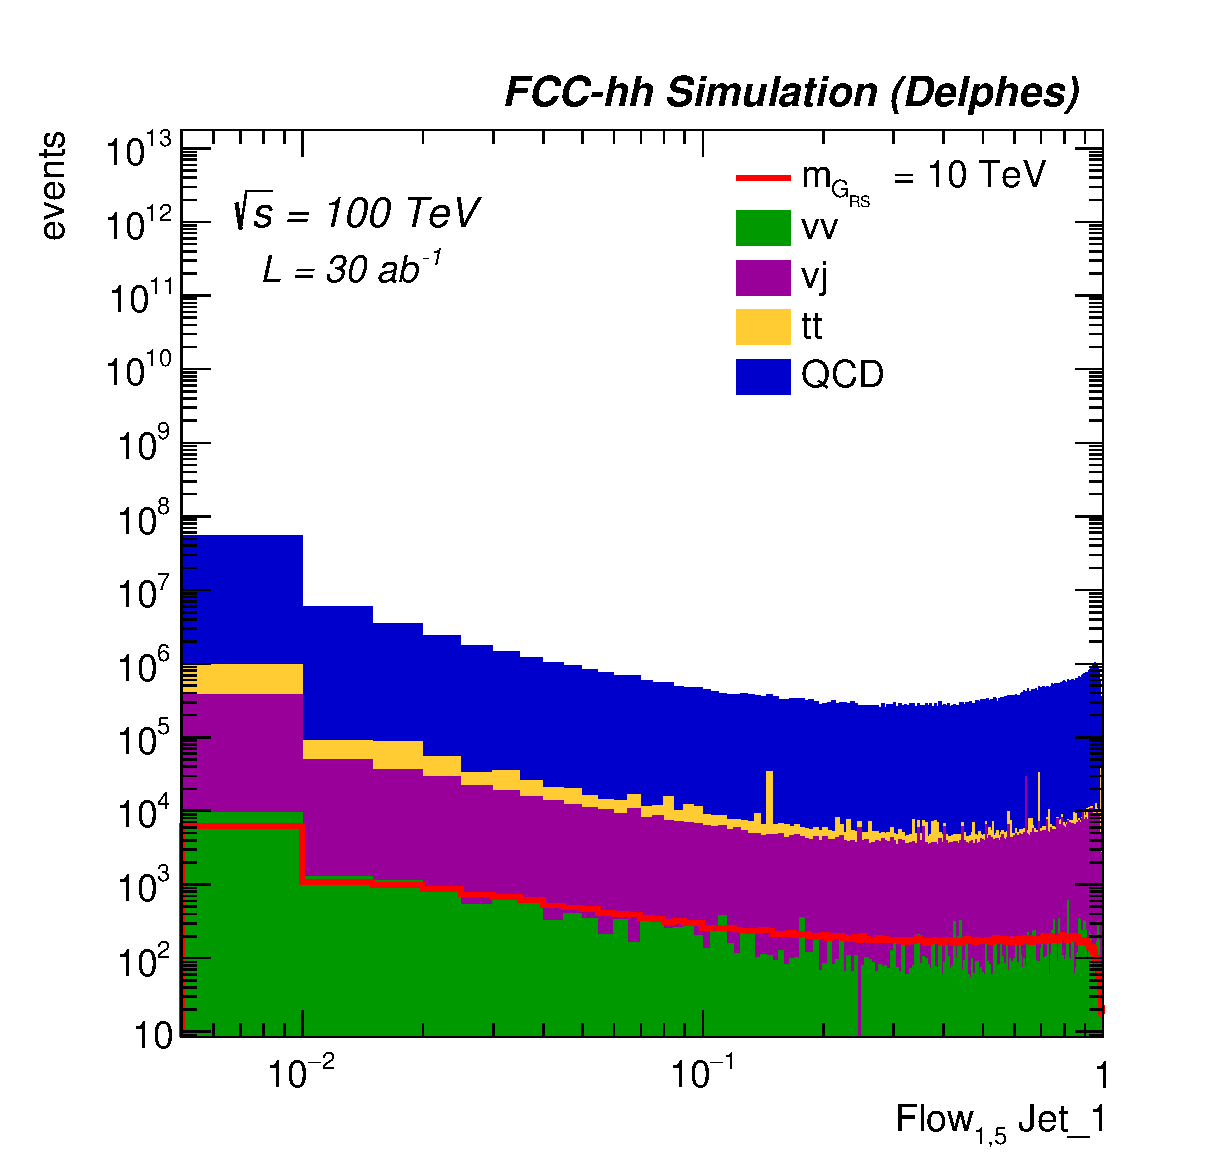
\includegraphics[width=0.33\textwidth]{Fig/TMVA/Jet1_Flow15_sel0_nostack_logx.eps}
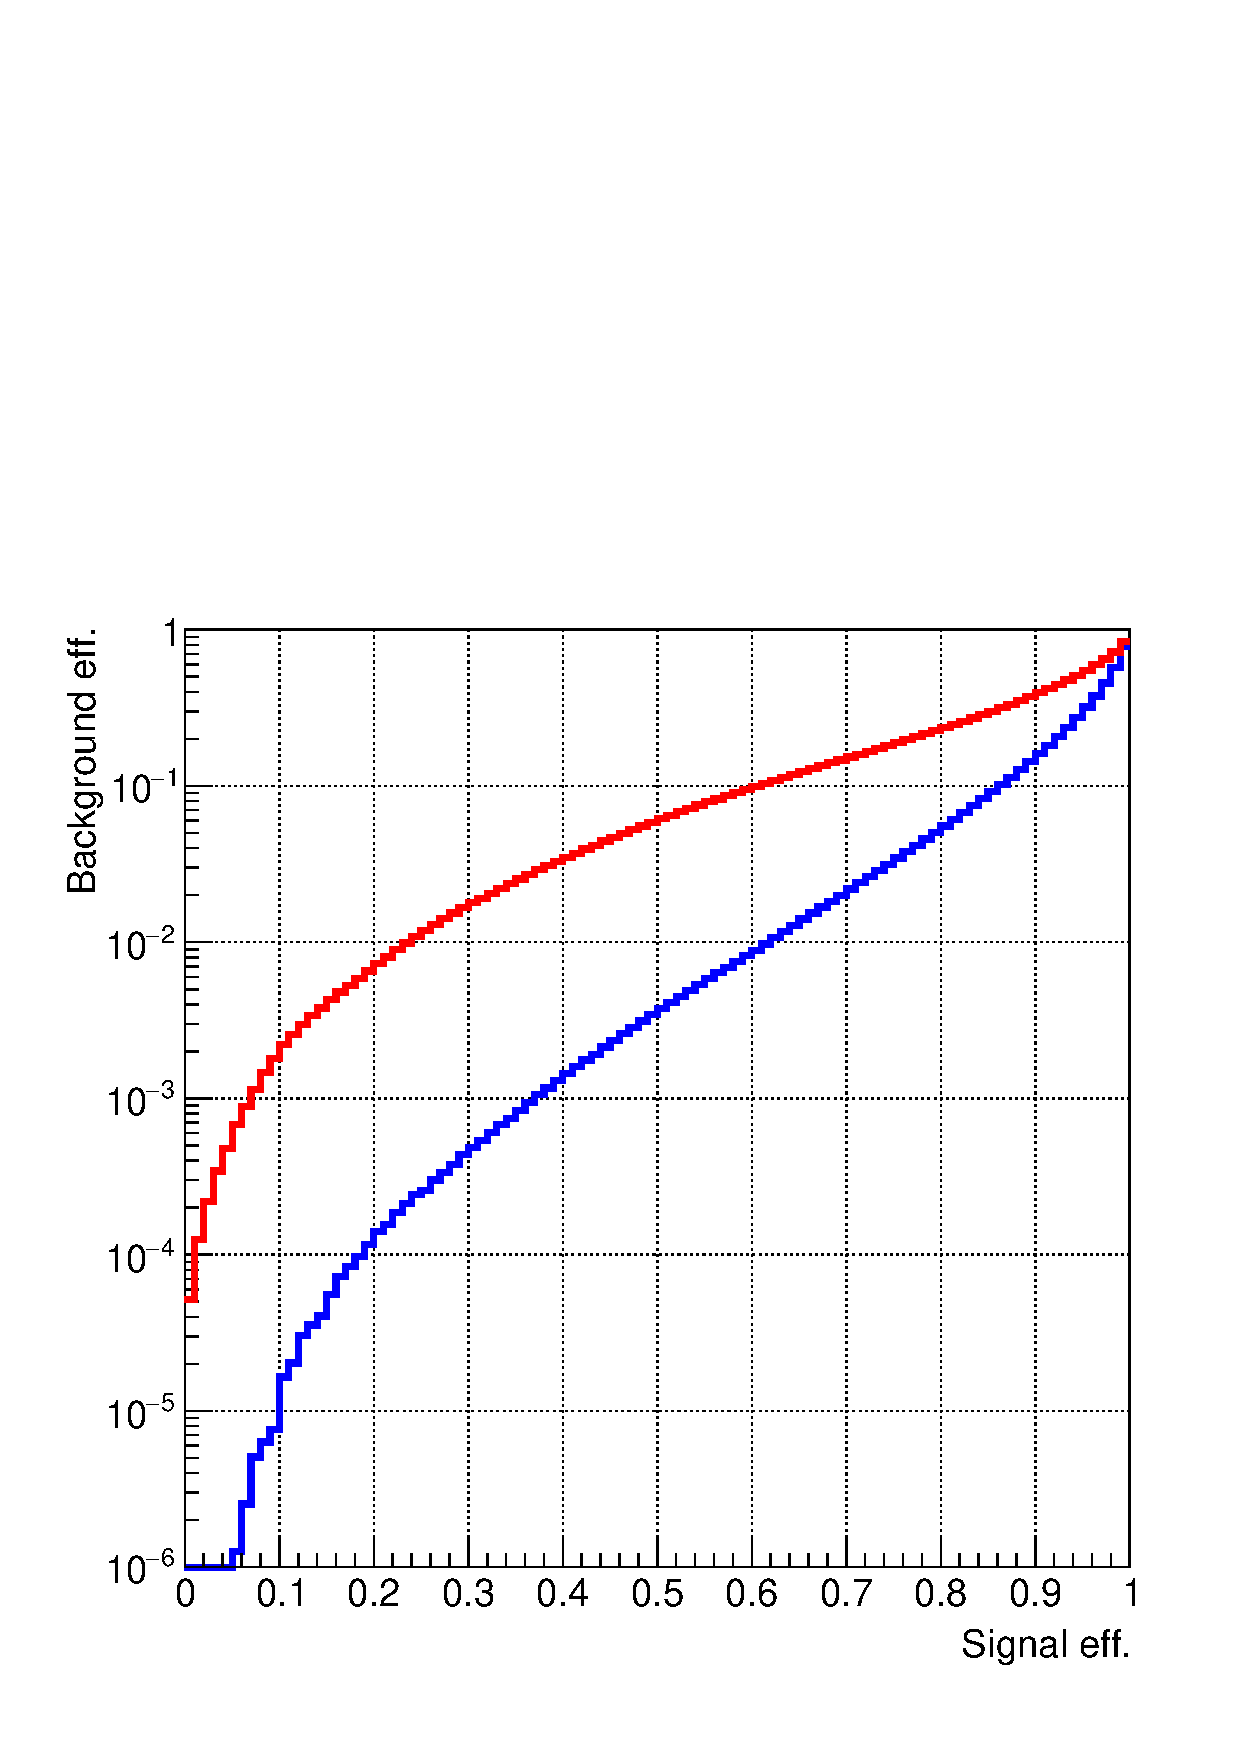
\includegraphics[width=0.33\textwidth,trim={0 0.5cm 0 0},clip]{Fig/TMVA/effQCD_vs_effWhadBlue_thadRed_log.pdf}
\caption{Left: Energy-flow ($E_{F}(1,0.05)$) observable for W and QCD jets. Right: Di-jet rejection versus signal efficiency for the two taggers, W in blue and top in red.}
\label{fig:TMVA_final_result}
\end{figure}

%\clearpage
%\newpage

%%%%%%%%%%%%%%%%%%%%%%%%%%%%%%%%%%%%%%%%%%%%%%%%%%%%%
\subsection{Tag Rate Function}
\label{subsec:trf}
The modeling of the backgrounds in the high tagging regimes is a challenging task. 
The requirement of $b$ tagging in some MC samples can drastically reduce the available statistics.
This shortage of events that pass the $b$-tagging cut in the signal regime, in conjunction with the large cross section of some of the backgrounds can lead to very spiky templates. 
\newline
To overcome this problem the tag rate function (TRF) method is introduced. 
By using the TRF method, no event is cut based on its $b$-tagging count, but instead all the events are weighted.
This weight can be interpreted as the probability of the given event to contain the desired number of $b$ jets. 
To achieve this, the tagging efficiency (a function of $\eta$, $\pt$ and true jet flavour) was
used to calculate the event weight based on the kinematics and flavour of the jets found in each event.
\newline
Given a jet with $\eta$, $\pt$ and flavour $f$, its tagging probability can be noted as:
\begin{equation*}
	\varepsilon \left(f,|\eta|,\pt\right)
\end{equation*}
\newline
For a given event with $N$ jets, its probability of containing exactly one $b$-tag jet can be computed as:
\begin{equation*}
	P_{=1} = \sum\limits_{i=1}^N \left( \varepsilon_{i} \prod\limits_{i \neq j} \left( 1 - \varepsilon_{j} \right) \right)
\end{equation*}
\newline
In the same way, it can be used to compute the probability for inclusive $b$-tag selections:
\begin{align*}
	P_{=0} &= \prod\limits_{i=1}^N \left( 1 - \varepsilon_{j} \right) \\
	P_{\geq 1} &= 1 - P_{=0}
\end{align*}
\newline
It was verify that the TRF methods agrees well with the direct tagging.

%%%%%%%%%%%%%%%%%%%%%%%%%%%%%%%%%%%%%%%%%%%%%%%%%%%%%
\subsection{Mass spectrum fit}
Despite the fact that very large amount of Monte-Carlo statistic has been simulated in bins of $\hht$
and the usage of techniques to save events with TRF methods,
there are still large statistical fluctuations from high weight events.
In order to reduce this effect, a function is used to fit the background distribution,
\begin{equation}
f(z)=p_1(1-z)^{p_2}z^{p_3}z^{p_{4}logz}
\end{equation}
where $z=m_{jj}/\sqrt{s}$. This fit is used in order to have a smooth shape for the backgrounds, while the normalisation is taken prior to the fit (see figure~\ref{fig:hadronicresonances_nofit}).

\begin{figure}[!htb]\centering
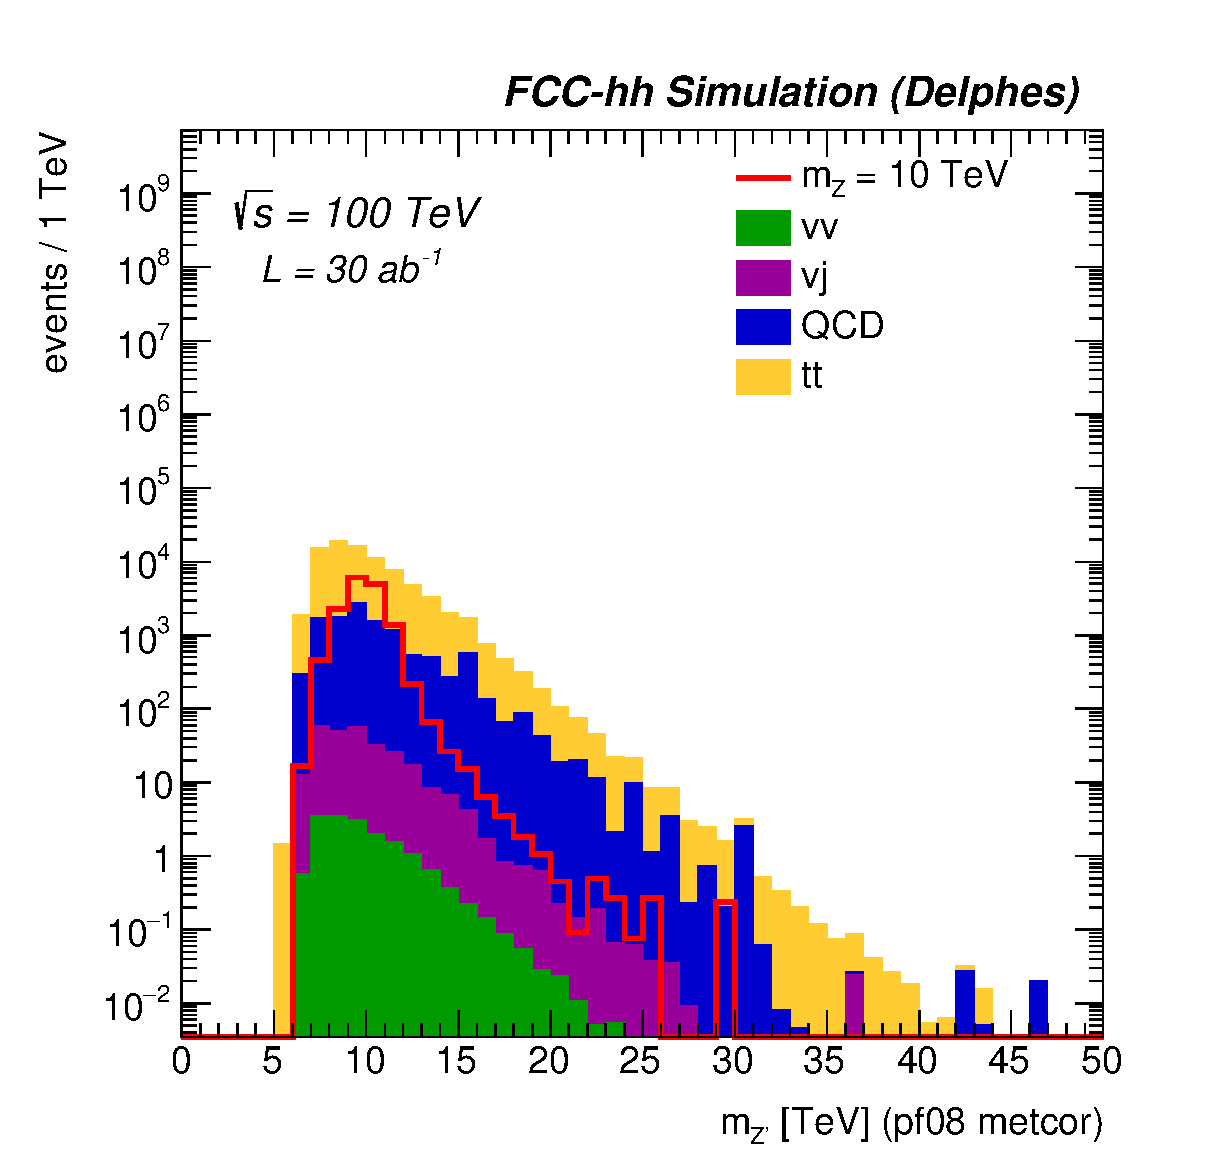
\includegraphics[width=0.33\columnwidth]{Fig/Zptt/Mj1j2_pf08_MetCorr_sel8_nostack_log.eps}
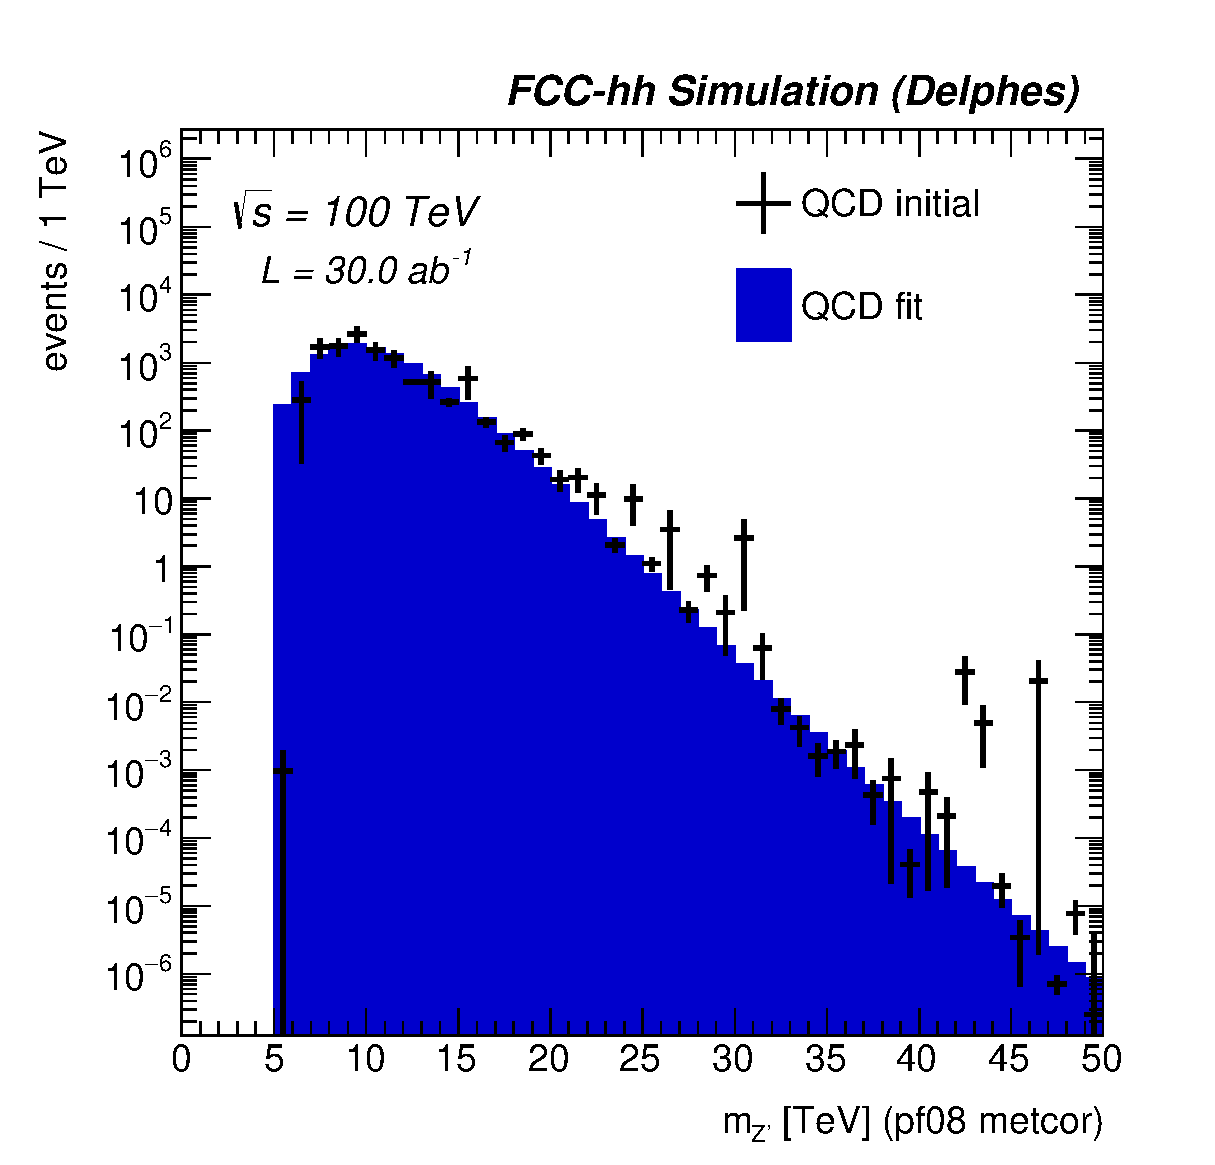
\includegraphics[width=0.33\columnwidth]{Fig/Zptt/Zptt_QCD_sel8_Mj1j2_pf08_MetCorr_fit.eps}
\caption{Invariant mass prior to fit.}
\label{fig:hadronicresonances_nofit}
\end{figure}

%%%%%%%%%%%%%%%%%%%%%%%%%%%%%%%%%%%%%%%%%%%%%%%%%%%%%
\subsection{Limit settings}
\label{subsec:limitsettings}

Develop here ?

%%%%%%%%%%%%%%%%%%%%%%%%%%%%%%%%%%%%%%%%%%%%%%%%%%%%%%
\section{Physics models}
\label{sec:physmodel}

Models with extended gauge groups often feature additional U(1) symmetries with corresponding heavy spin-1 bosons. These bosons, generally referred to as $\Zp$, would manifest as a narrow resonance through
its  decay,  in  the  dilepton  mass  spectrum.   
Among  these  models  are  those  inspired  by  Grand  Unified Theories, which are 
motivated by gauge unification or a restoration of the left–right symmetry violated
by the weak interaction. Examples are the $\Zp$
bosons of the E6 motivated [1, 2] theories as well as Minimal models [3].  
The Sequential Standard Model (SSM) [2] posits a $\ZpSSM$ boson with couplings to fermions
that are identical to those of the SM $\Z$ boson. This model is a good benchmark as the 
results can be interpreted in the context of other models of new physics, and is useful 
for comparing the sensitivity of different experiments.
 % useless because of sections/BSM-models
%%%%%%%%%%%%%%%%%%%%%%%%%%%%%%%%%%%%%%%%%%%%%%%%%%%%%
\section{Analyses at 100 TeV FCC-hh}
\label{sec:ana100tev}

%%%%%%%%%%%%%%%%%%%%%%%%%%%%%%%%%%%%%%%%%%%%%%%%%%%%%
%%%%%%%%%%%%%%%%%%%%%%%%%%%%%%%%%%%%%%%%%%%%%%%%%%%%%
\subsection{Leptonic resonances : ee, \texorpdfstring{$\mu\mu$}{uu}, \texorpdfstring{$\tau\tau$}{tt}}
\label{subsec:lepreso}

%%%%%%%%%%%%%%%%%%%%%%%%%%%%%%%%%%%%%%%%%%%%%%%%%%%%%%%%%%%%%%%%%%%%%%%%%%%%%%%%%%%%%%%%%%%%
\subsubsection{Introduction}
Models with extended gauge groups often feature additional U(1) symmetries with corresponding heavy spin-1 bosons. These bosons, generally referred to as $\Zp$, would manifest themselves as a narrow resonance in the dilepton mass spectrum. Among these models are those inspired by Grand Unified Theories, motivated by gauge unification or a restoration of the left-right symmetry violated by the weak interaction. Examples include the $\Zp$ bosons of the E6 motivated theories~\cite{London:1986jz,Joglekar:2016yap,Langacker:2008yv,Hewett:1988xc} and Minimal models~\cite{Salvioni:2009mt}. The Sequential Standard Model (SSM)~\cite{Langacker:2008yv} posits a $\ZpSSM$ boson with couplings to fermions that are identical to those of the Standard Model $\Z$ boson.

The decay products of heavy resonances are in the multi-TeV regime and the capability to reconstruct their momentum imposes stringent requirement on the detector design. In particular, reconstructing the track curvature of multi-TeV muons requires excellent position resolution and a large lever arm. In this section, the expected sensitivity is presented for a \Zpll\ (where $\ell=\mathrm{e},\mu$) and \Zptata\ separately.

%%%%%%%%%%%%%%%%%%%%%%%%%%%%%%%%%%%%%%%%%%%%%%%%%%%%%%%%%%%%%%%%%%%%%%%%%%%%%%%%%%%%%%%%%%%%
\subsubsection{Event Selection}
Events are required to contain two leptons with $\pt > 1$~TeV, $|\eta|$<4 and an invariant mass $\mll > 2.5$~TeV. For di-$\tau$ final state we focus on the most sensitive fully hadronic channel only. The di-$\tau$ event selection requires two jets with $p_{T} > 0.5$>~TeV and $|\eta|<2.5$ identified as $\tau$'s. To ensure no overlap between the $\ell$ and $\tau$ final states, jets containing leptons with $\pt > 100$~GeV are vetoed. Finally, requirements of $\Delta \phi(\tau_1, \tau_2)> 2$ and $2.5<\Delta R(\tau_1, \tau_2)<4$ are applied.
Mass dependent cuts applied to maximise the signal to background ratio are summarised in Table~\ref{tab:leptonicresonances:selectiontautau}.

Figure~\ref{figure:leptonicresonances:masses} (left and center) shows the invariant mass for a 30~TeV signal for the $ee$ and $\mu\mu$ channels, and the yields can be found in Table~\ref{tab:leptonicresonances:yieldstautau}. The mass resolution is better for the ee channel, as expected. Figure~\ref{figure:leptonicresonances:masses} (right) shows the transverse mass~\footnote{the transverse mass is defined as $m_{T}  =  \sqrt{2\ptZp*\met*(1-cos\Delta\phi(\Zp,\met))} $}
of a 10~TeV signal for the $\tau\tau$ channel, and the yields can be found in Table~\ref{tab:leptonicresonances:yieldsll}.
Several proxies for the true resonance mass have been tested, such as the invariant mass of the two taus, with and without correction for the missing energy. The transverse mass provided the best sensitivity and was therefore used to set limits and determine the discovery reach.

\begin{table}[htbp]
   \centering
\begin{tabular}{|l|l|c|r|}
  \hline
  \hline
   $\Zp$ mass [TeV] &  $\Delta \phi(\tau_1, \tau_2)$&  $\Delta R(\tau_1, \tau_2)$ & $\met$\\
  \hline
  $4-8$ & > 2.4 & > 2.5 and < 3.5 & > 400 GeV\\
  $10$ & > 2.4 & > 2.7 and < 4 & > 300 GeV\\
  $12-14$ & > 2.6 & > 2.7 and < 4 & > 300 GeV\\
  $16-18$ & > 2.7 & > 2.7 and < 4 & > 300 GeV\\
  $>18$ & > 2.8 & > 3 and < 4 & > 300 GeV\\
  \hline
  \hline
  \end{tabular}
  \caption{List of mass dependent cuts optimised to maximise the sensitivity for the \Zptata\ search.}
  \label{tab:leptonicresonances:selectiontautau}
\end{table}

\begin{table}[htbp]
   \centering
\begin{tabular}{|l|r|r|}
  \hline
  \hline
 & ee & $\mu\mu$  \\
  \hline
  Drell-Yan & 206882.9 & 236597.9 \\
  \hline
  $\Zp$ 4~TeV & 1421357.9    & 1598969.4 \\
  $\Zp$ 6~TeV & 349922.4  & 393117.6\\
  $\Zp$ 8~TeV &   115043.5 & 129698.7 \\
  $\Zp$ 10~TeV &  45423.5 & 50873.3 \\
  $\Zp$ 20~TeV &  1192.3 & 1411.5\\
  $\Zp$ 30~TeV &  88.2 & 107.6\\
  $\Zp$ 40~TeV &  11.7 & 14.1 \\
  $\Zp$ 50~TeV &  3.2 & 3.7\\
  \hline
  \hline
\end{tabular}
  \caption{Expected number of events for the \Zpee\ and \Zpmumu\ analysis after the full event selection for the various \Zp\ mass hypotheses}
  \label{tab:leptonicresonances:yieldsll}
\end{table}

\begin{table}[htbp]
   \centering
\begin{tabular}{|l|r|r|r|}
  \hline
  \hline
$\Zp$ mass [TeV]  & signal &  Drell-Yan & Di-jet \\
  \hline
  $4$     &  51479.5 &  \multirow{3}{*}{5669.2} &   \multirow{3}{*}{875561.7} \\
  $6$     &  22294.3  & &\\
  $8$     &  9140.7  &  &\\
  \hline

  $10$      & 5398.8 & 9008.3 & 2040422.6 \\
  \hline

  $12$ &  2261.4&  \multirow{3}{*}{8946.8} &  \multirow{3}{*}{1982792.8}  \\
  $14$ &  1040.9&  &  \\
  \hline

  $16$ &  489.6&  \multirow{3}{*}{8826.3} &  \multirow{3}{*}{1915211.5} \\
  $18$ &  251.9&  &  \\
    \hline

  $20$    &  122.6& \multirow{3}{*}{7777.2} & \multirow{3}{*}{1609435.6}   \\
  $25$    &  27.5 &  &  \\
  $30$    &  7.1 &  &  \\
  \hline
  \hline
\end{tabular}
  \caption{Expected number of events for the \Zptata\ analysis after the full event selection for the various \Zp\ mass hypotheses}
  \label{tab:leptonicresonances:yieldstautau}
\end{table}

\begin{figure}[!htb]
  \centering
  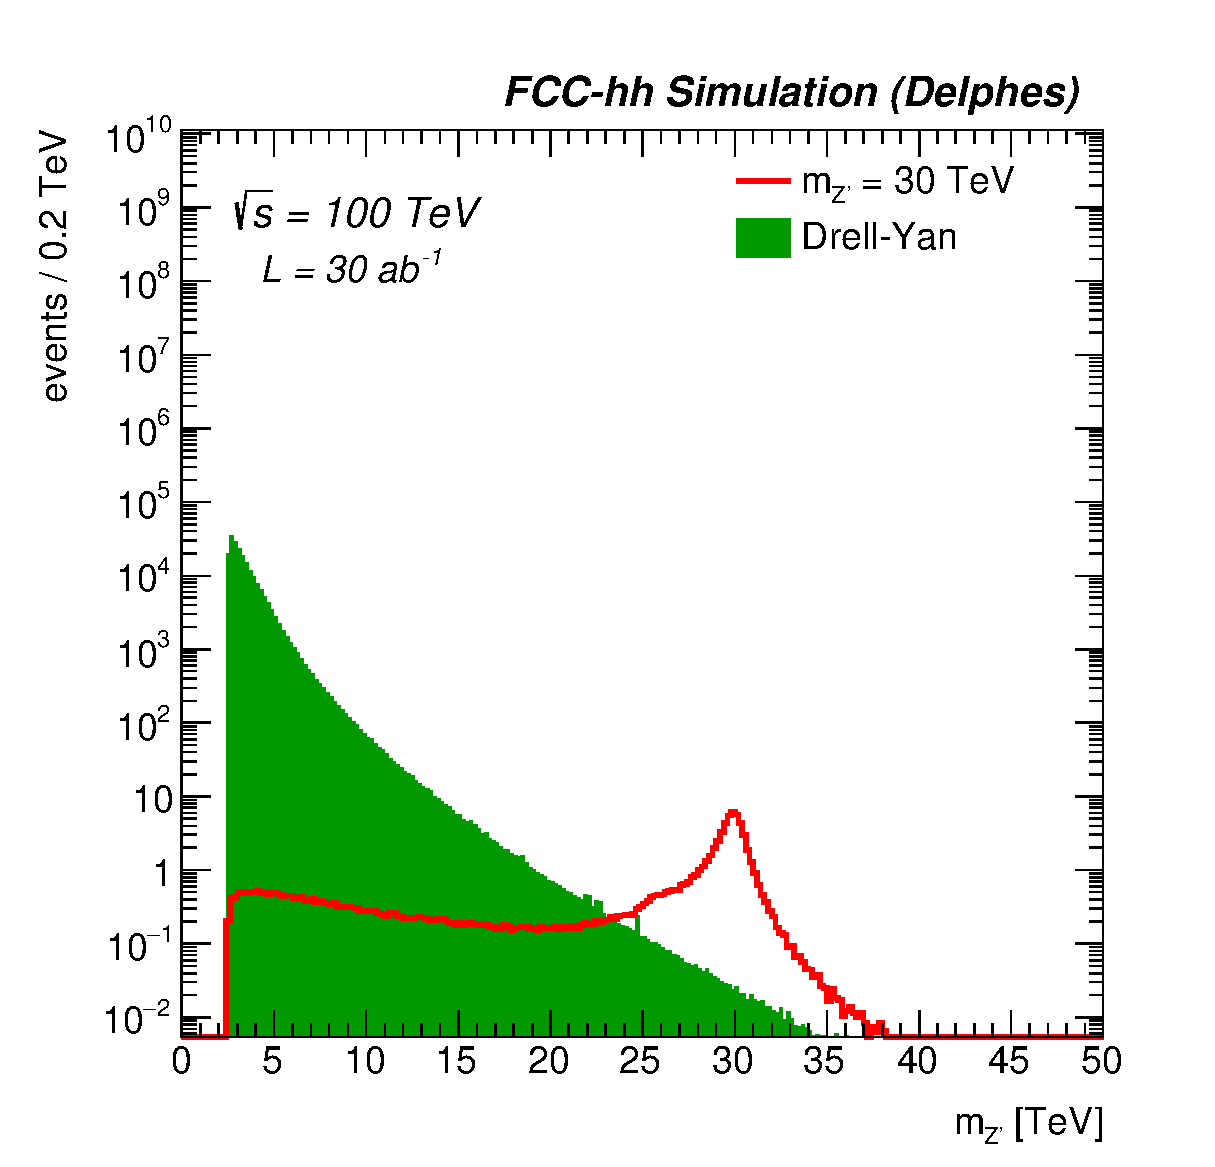
\includegraphics[width=0.32\columnwidth]{Fig/mzp_sel0_nostack_log_ee.eps}
  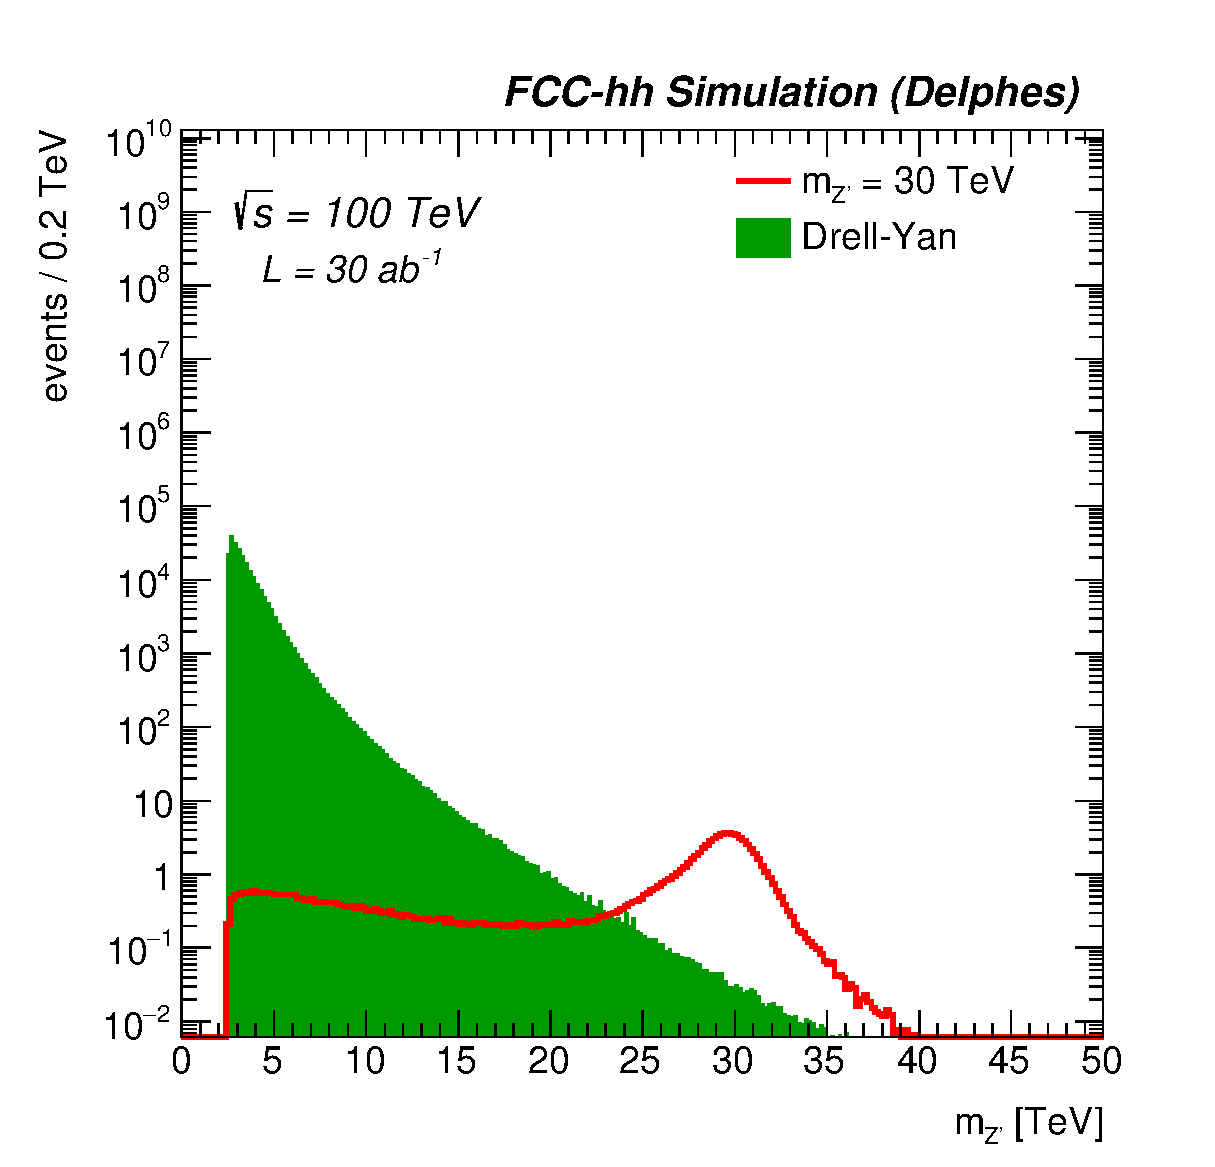
\includegraphics[width=0.32\columnwidth]{Fig/mzp_sel0_nostack_log_mm.eps}
  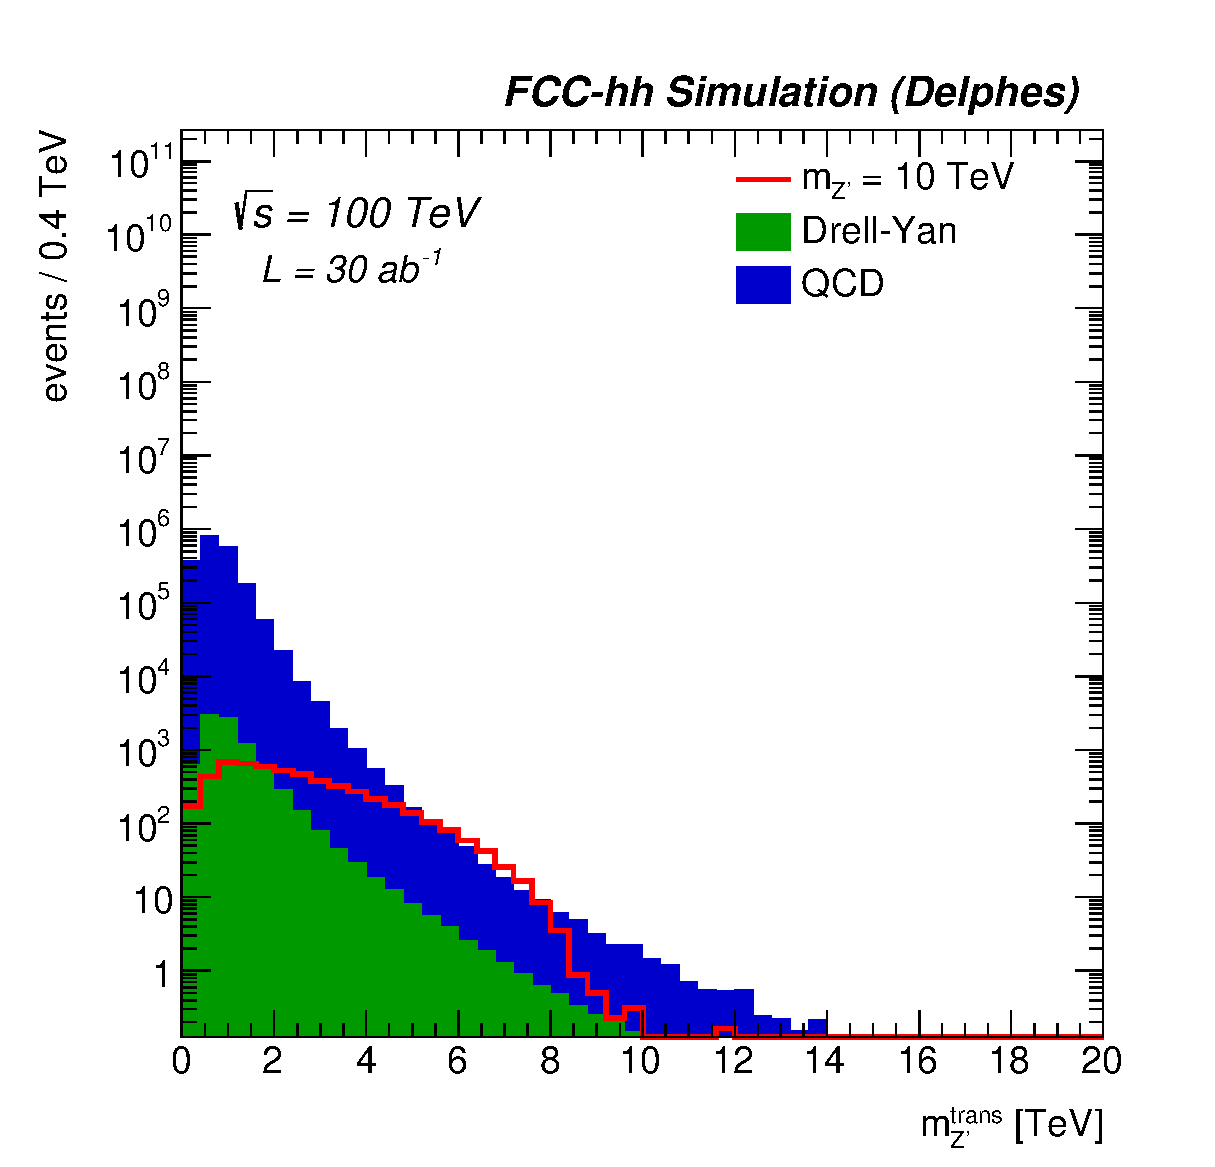
\includegraphics[width=0.32\columnwidth]{Fig/mt_finalsel_nostack_log.eps}
  \caption{Left, center: Invariant mass for a 30~TeV signal after full event selection for ee channel (left) and $\mu\mu$ channel (center). Right: Transverse mass for a 10~TeV signal after full event selection for the $\tau\tau$ channel. }
  \label{figure:leptonicresonances:masses}
\end{figure}
%\MS{need editing / style}

%%%%%%%%%%%%%%%%%%%%%%%%%%%%%%%%%%%%%%%%%%%%%%%%%%%%%%%%%%%%%%%%%%%%%%%%%%%%%%%%%%%%%%%%%%%%
\subsubsection{Results and discussion}
Hypothesis testing is performed using a modified frequentist method based on a profile likelihood that takes into account the systematic uncertainties as nuisance parameters that are fitted to the expected Monte-Carlo. For the $ee$ and $\mu\mu$ analyses, the di-lepton invariant mass is used as the discriminant, while for the $\tau\tau$ channel the transverse mass is used. A 50\% uncertainty on the background normalisation is assumed.

Figure~\ref{figure:leptonicresonances:resultsll} shows the exclusion limit obtained \intlumifcc\ of data for the ee alone (top left), $\mu\mu$ alone (top right) and combination of (ee,$\mu\mu$) channels (bottom left). Figure~\ref{figure:leptonicresonances:resultsll} (bottom right) shows the integrated luminosity required to reach a $5\sigma$ discovery for the leptonic resonances as a function of the mass of the heavy resonance. The \Zpee\ and \Zpmumu\ channel display very similar performance, due to the low background rates. We conclude therefore that the reference detector design features near to optimal performance for searches involving high \pT\ muon final states. Figure~\ref{figure:leptonicresonances:resultstautau} shows the exclusion limits for 30 ab$^{-1}$ of data (left) and the required integrated luminosity
versus mass to reach a $5\sigma$ discovery (right) for the di-tau resonances.

The discovery potential for high mass resonances decaying to $ee$, $\mu\mu$ and $\tau\tau$ has been studied using as a benchmark the \ZpSSM\ model. The very large centre of mass energy provides a correspondingly large mass reach. For the $ee$ and $\mu\mu$ cases masses up to 42~TeV can be excluded or discovered. Heavy resonance decaying to $\tau$ leptons reconstructed in the hadronic decay mode are more challenging, but we would be able to probe massses up to 18~TeV.

\begin{figure}[!htb]
  \centering
  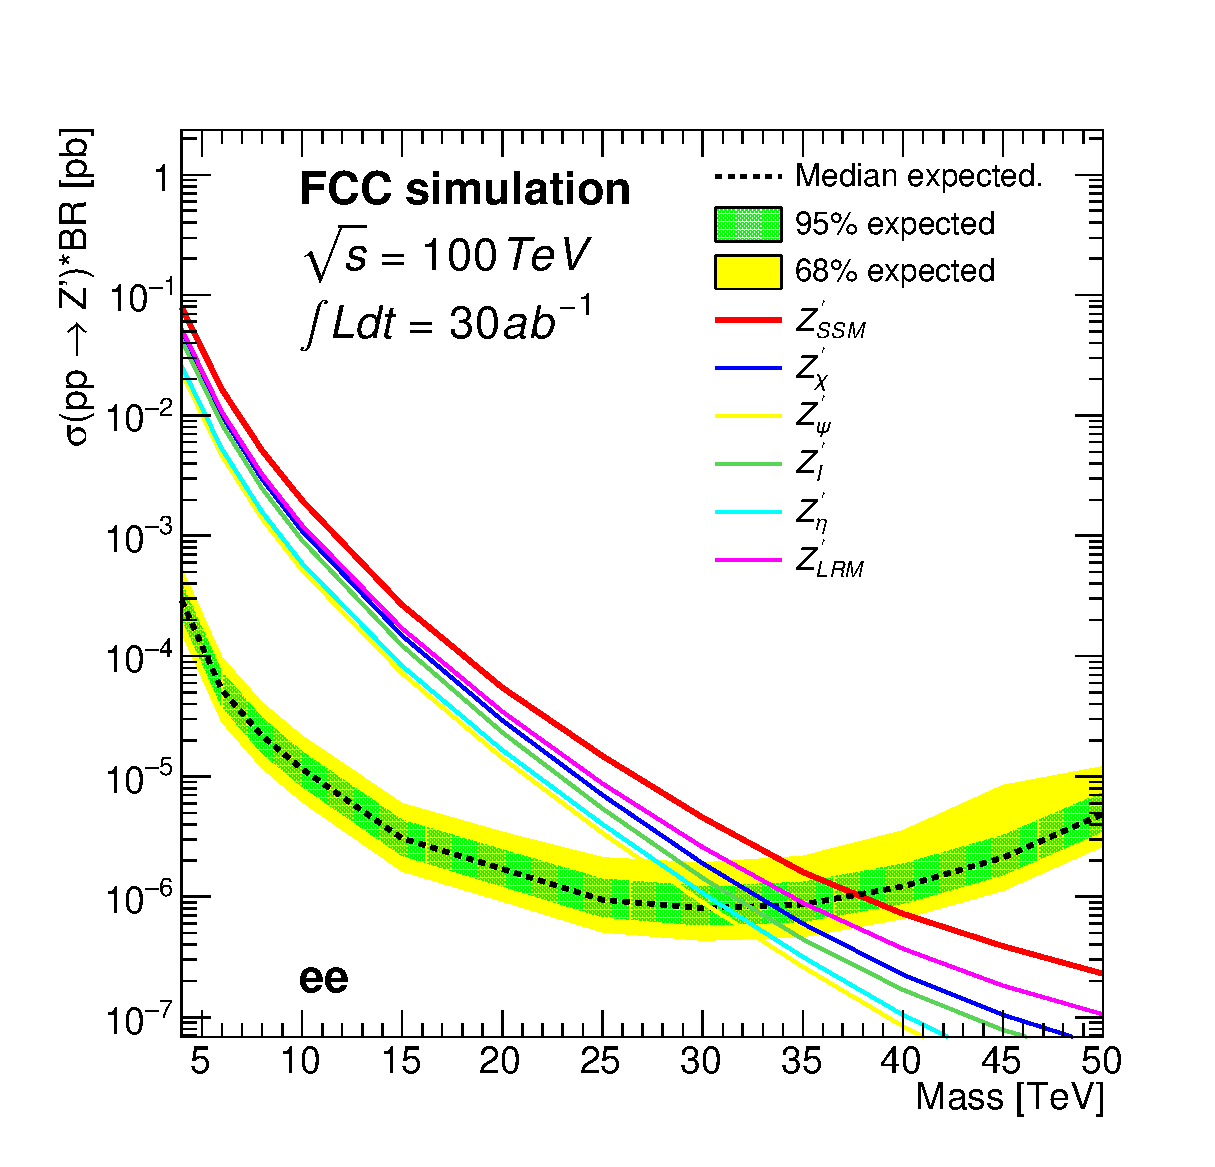
\includegraphics[width=0.33\columnwidth]{Fig/lim_Zprime_ee_fcc_v02_allxs.eps}
  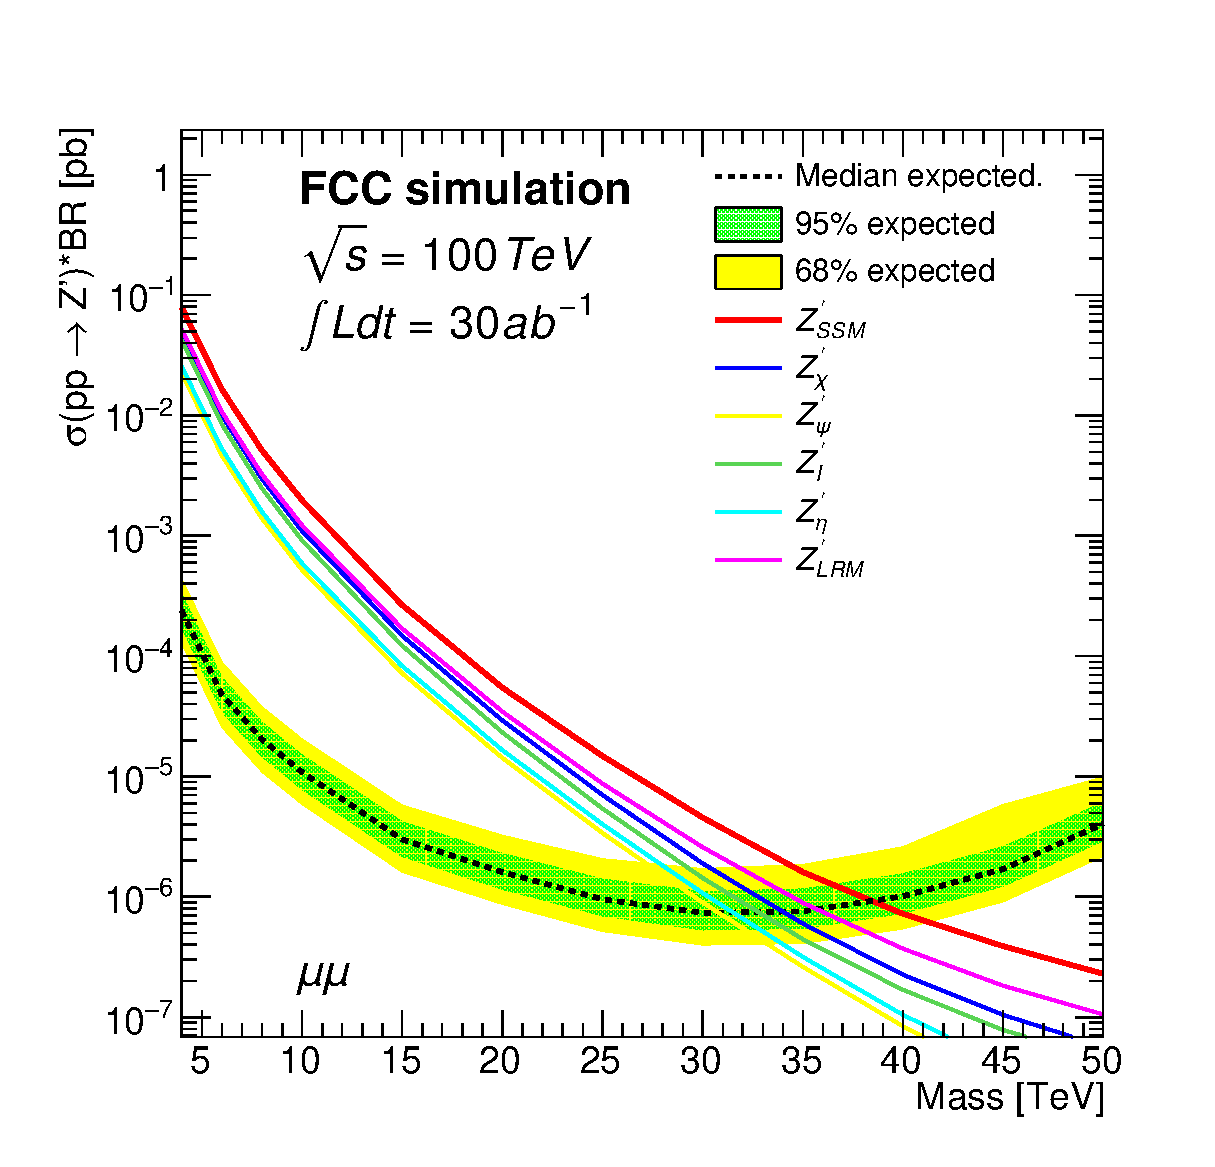
\includegraphics[width=0.33\columnwidth]{Fig/lim_Zprime_mumu_fcc_v02_allxs.eps}
  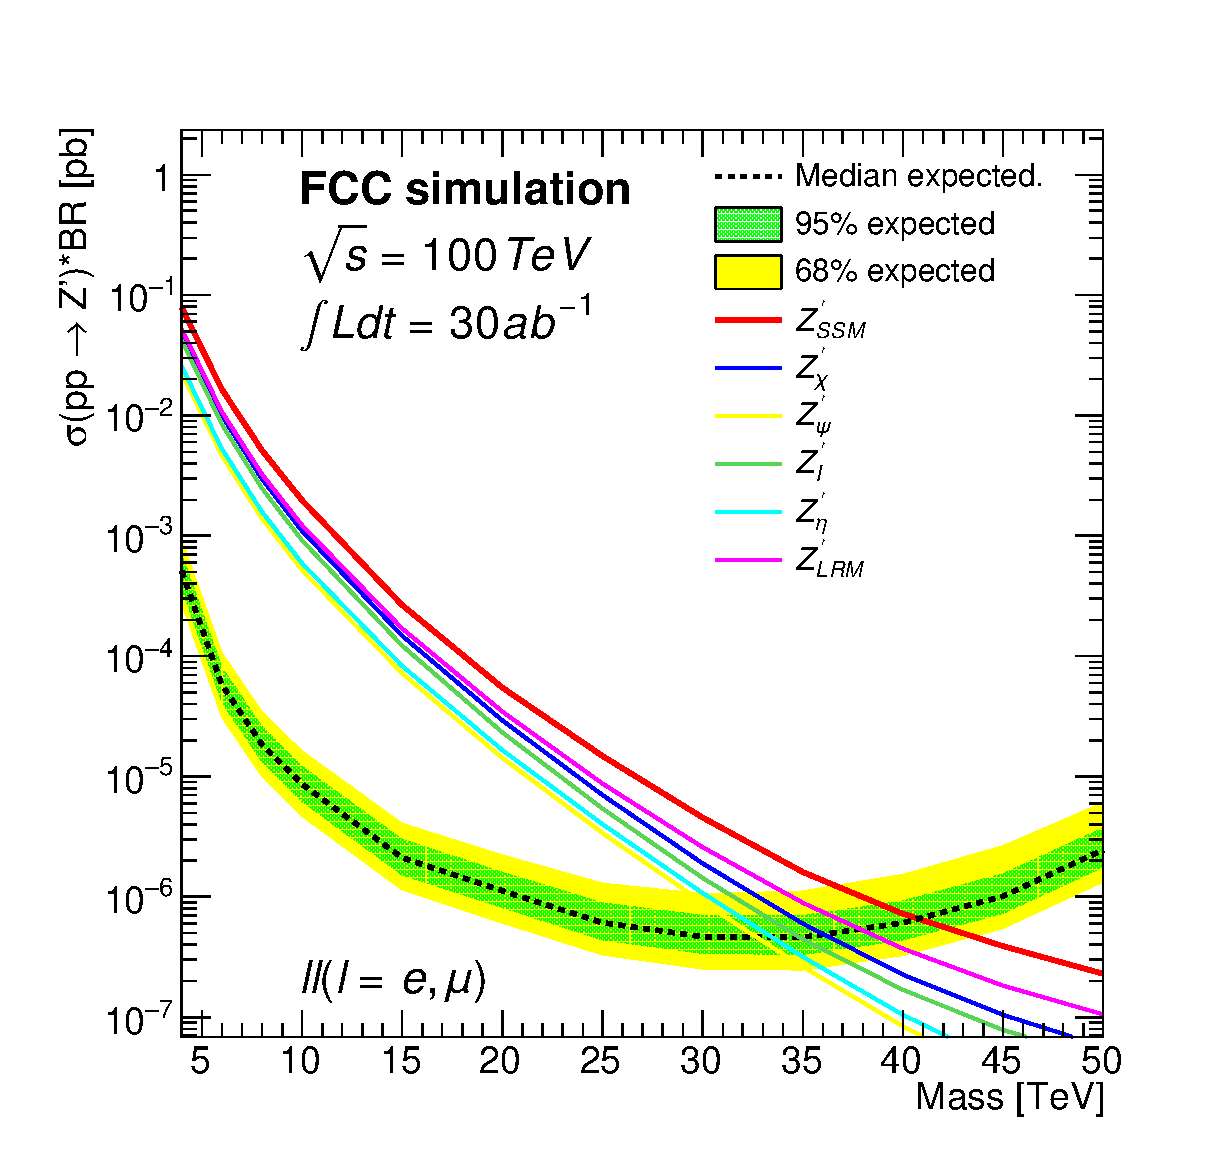
\includegraphics[width=0.33\columnwidth]{Fig/lim_Zprime_ll_fcc_v02_allxs.eps}
  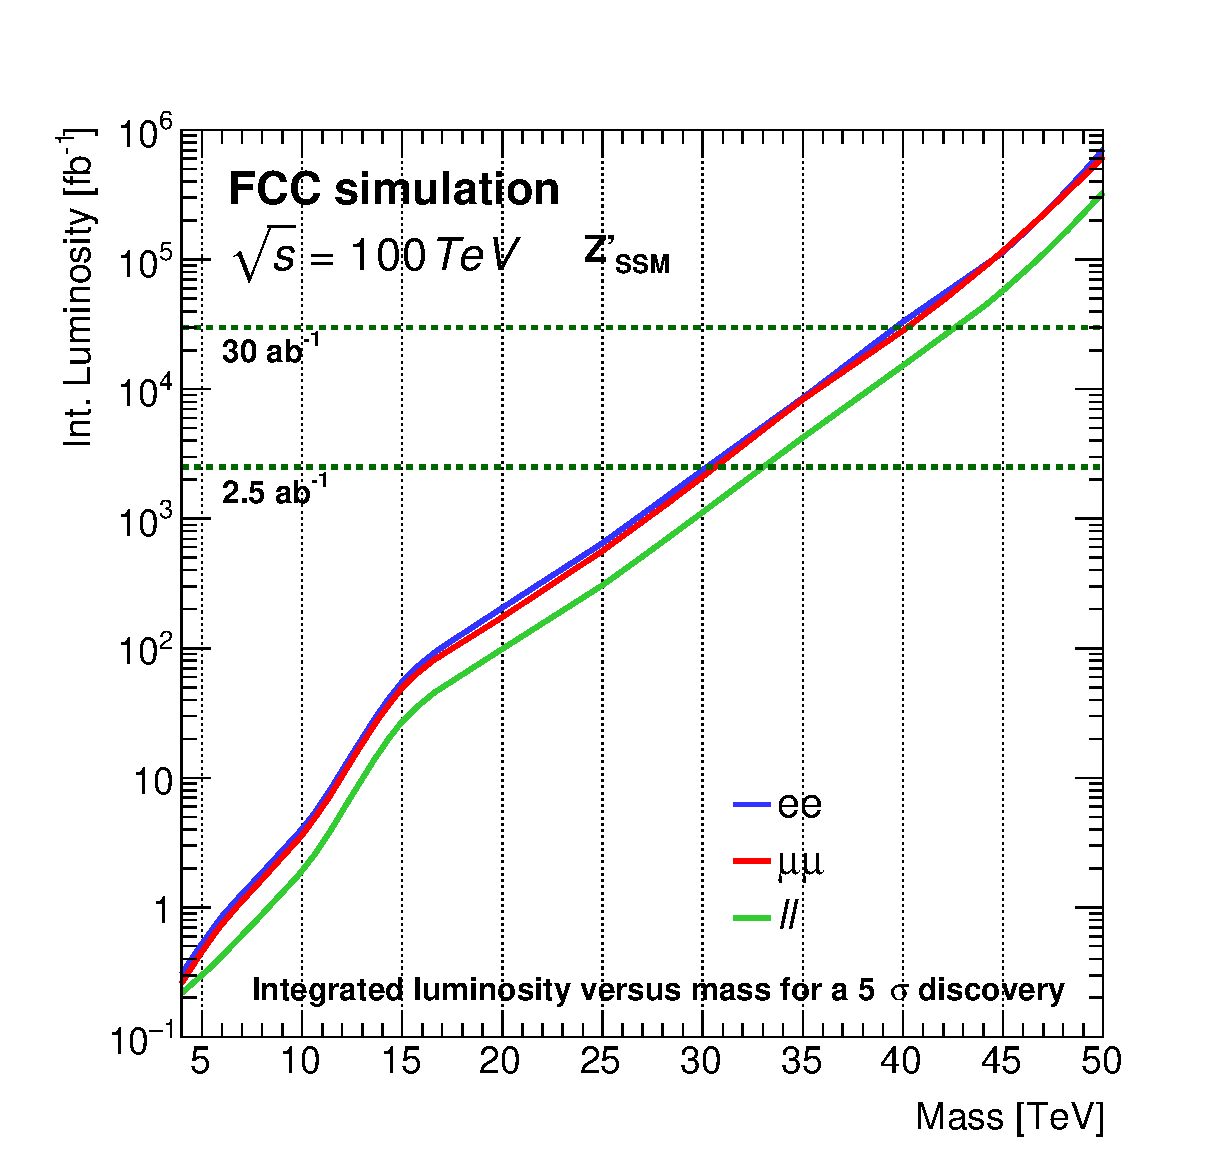
\includegraphics[width=0.33\columnwidth]{Fig/DiscoveryPotential_ll_comb_rootStyle.eps}
  \caption{Limit versus mass for the di-lepton (ee,$\mu\mu$) channel (left) and luminosity for a $5\sigma$ discovery (right) comparing ee,$\mu\mu$ and combined channels. }
  \label{figure:leptonicresonances:resultsll}
\end{figure}

\begin{figure}[!htb]
  \centering
  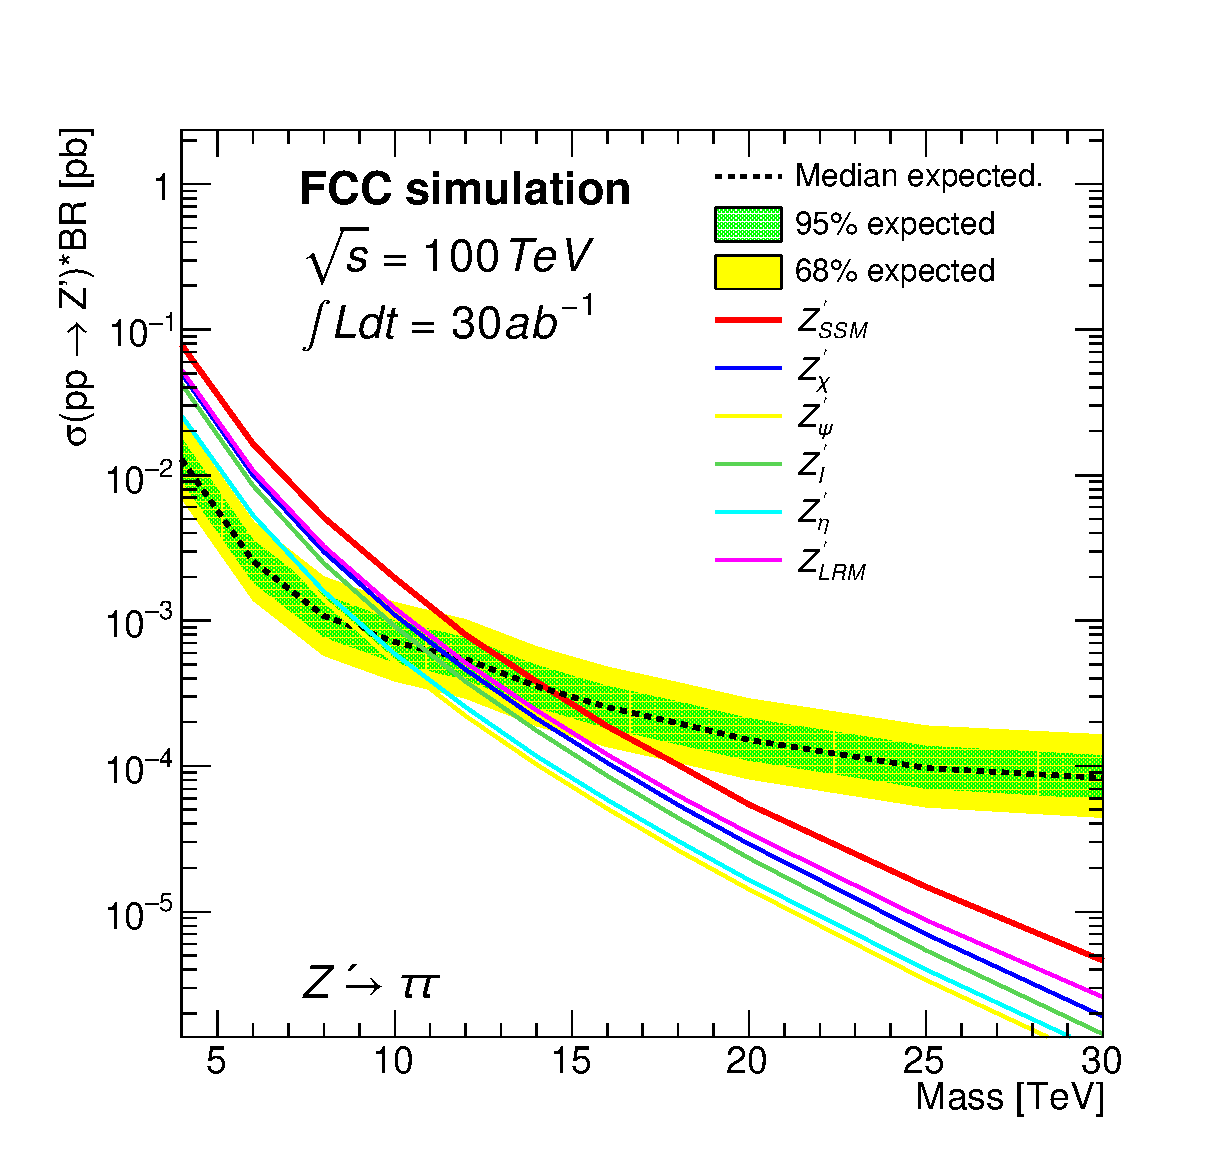
\includegraphics[width=0.33\columnwidth]{Fig/lim_Zprime_tautau_fcc_v02_allxs.eps}
  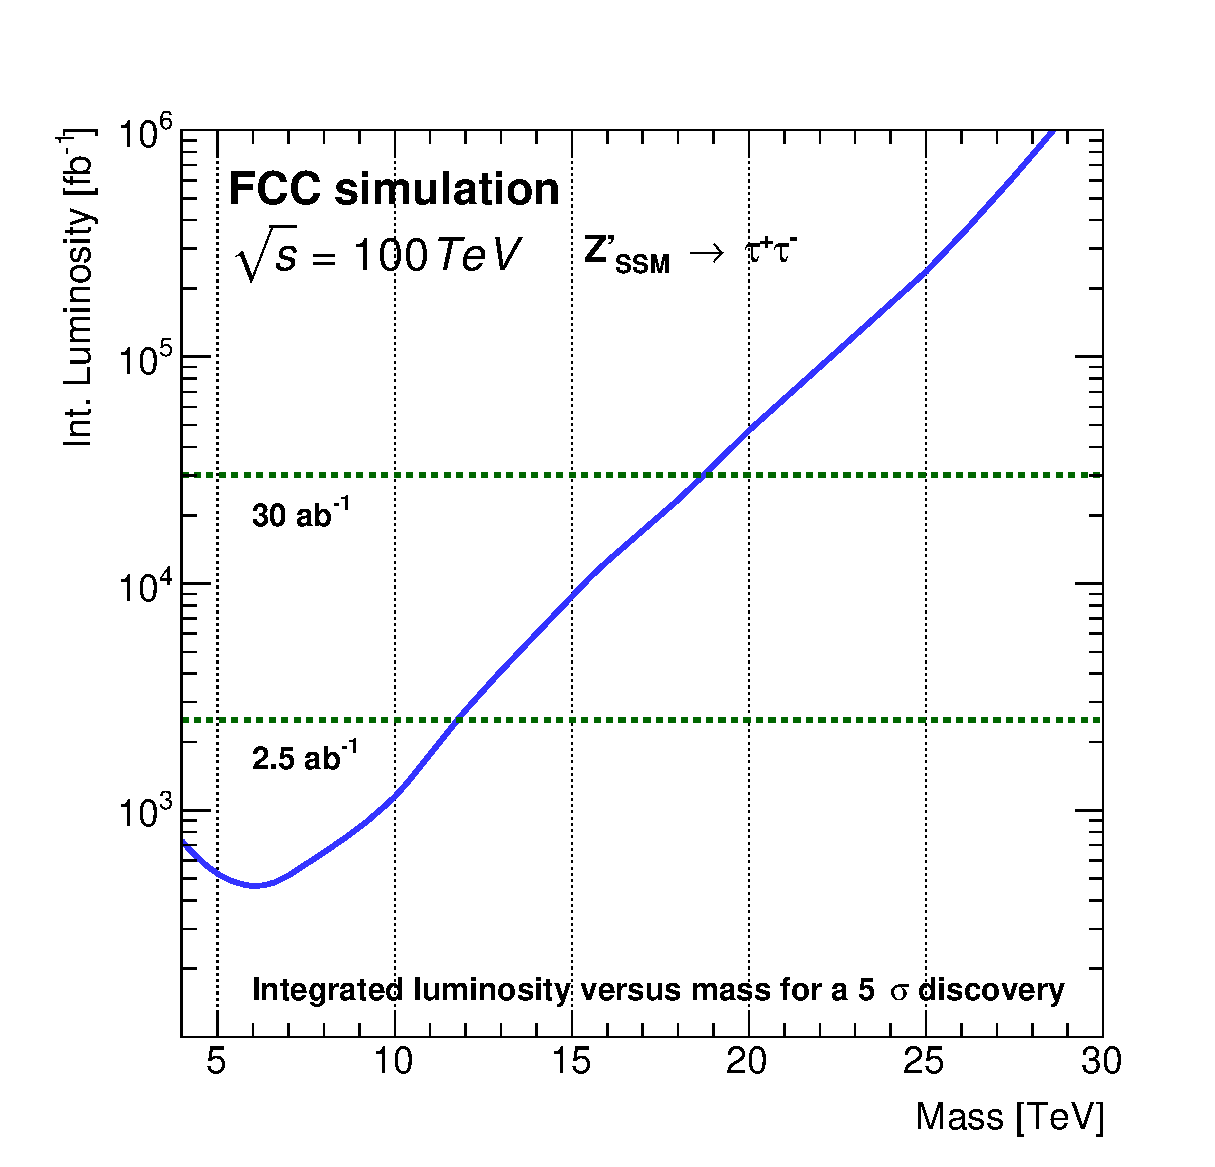
\includegraphics[width=0.33\columnwidth]{Fig/DiscoveryPotential_tautau_rootStyle.eps}
  \caption{Limit versus mass for the di-tau channel (left) and luminosity for a $5\sigma$ discovery (right). }
  \label{figure:leptonicresonances:resultstautau}
\end{figure}


\subsection{\texorpdfstring{$\mu\mu$}{uu} non-resonant interpretations}
LHCb measurements in $B\rightarrow~K^*\mu~+\mu~-$ decays are somewhat discrepant with Standard Model predictions~\cite{Aaij:2014ora,Aaij:2017vbb}. They may be harbingers of new physics at an energy scale potentially accessible to direct discovery. The flavour anomaly (f.a.) model $Z'$ and t-channel LQ interpretations from~\cite{Allanach:2017bta} are studied in this section.
\newline
The selection strategy is the same as the $Z'\rightarrow~\mu^+\mu^-$ in section~\ref{subsec:lepreso}. The only difference is the increase of lepton momentum threshold from 1 to 1.2 TeV.
\newline
Figure~\ref{figure:leptonicresonances:resultsmumu_flav} ($Z'$ f.a.) and ~\ref{figure:leptonicresonances:resultsmumu_flav} (t-channel LQ) show the invariant mass of the $\mu^+\mu^-$ system (left), the exclusion limit obtained \intlumifcc\ (middle) and the integrated luminosity required to reach a $5\sigma$ discovery for the two scenarios as a function of the mass of the $\mu^+\mu^-$ system (right).
It is found that $Z'$ is visible and LQ would need to search for pair production.

\begin{figure}[!htb]
  \centering
  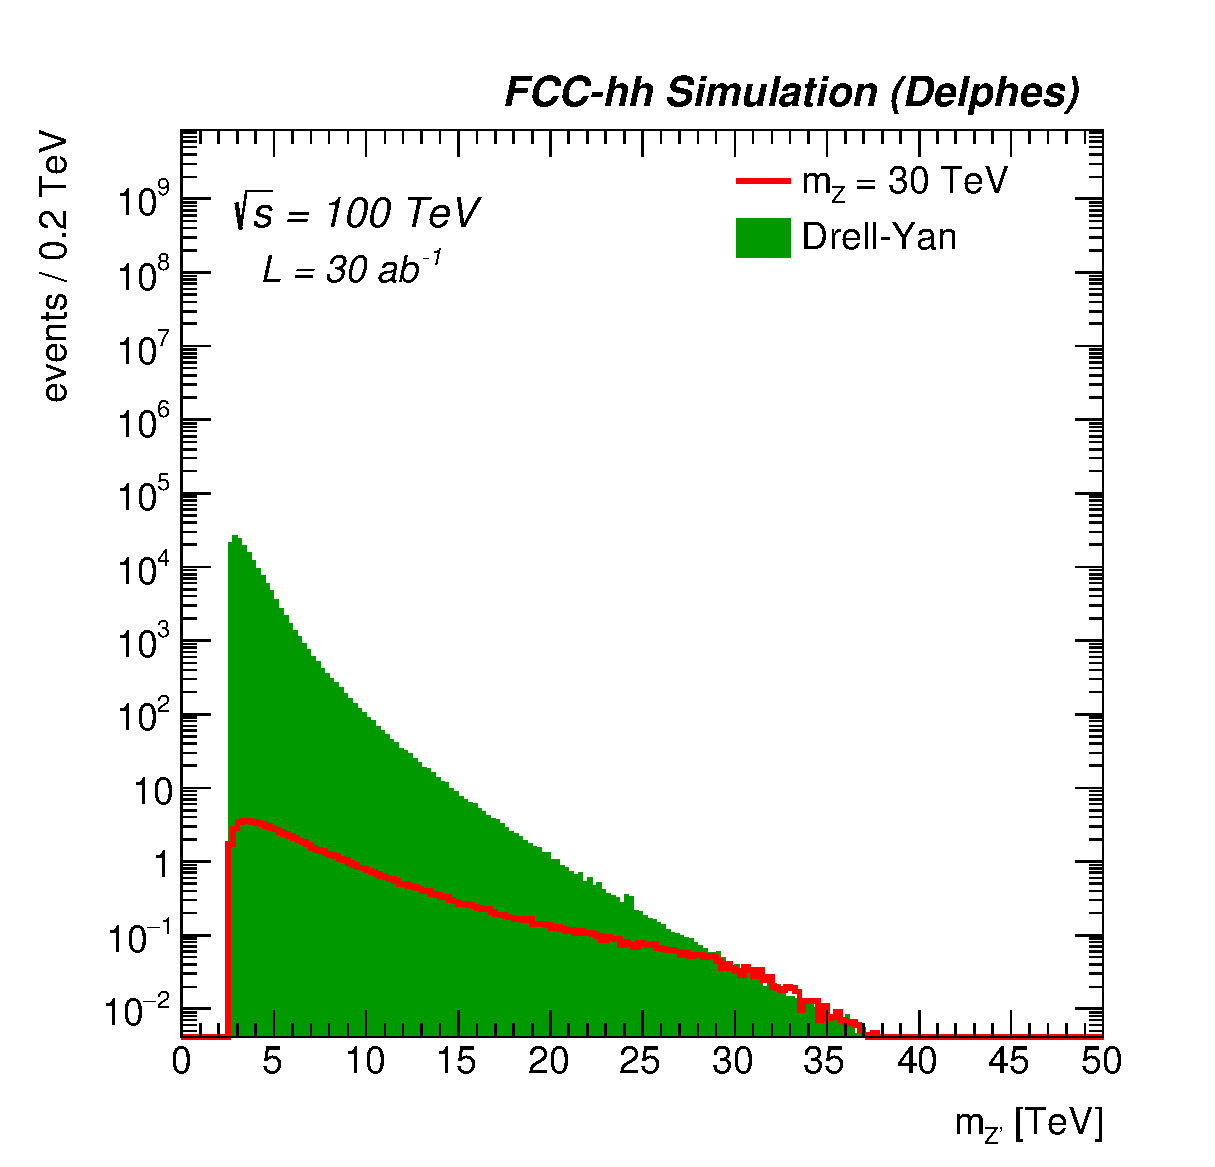
\includegraphics[width=0.32\columnwidth]{Fig/mzp_sel0_nostack_log.eps}
  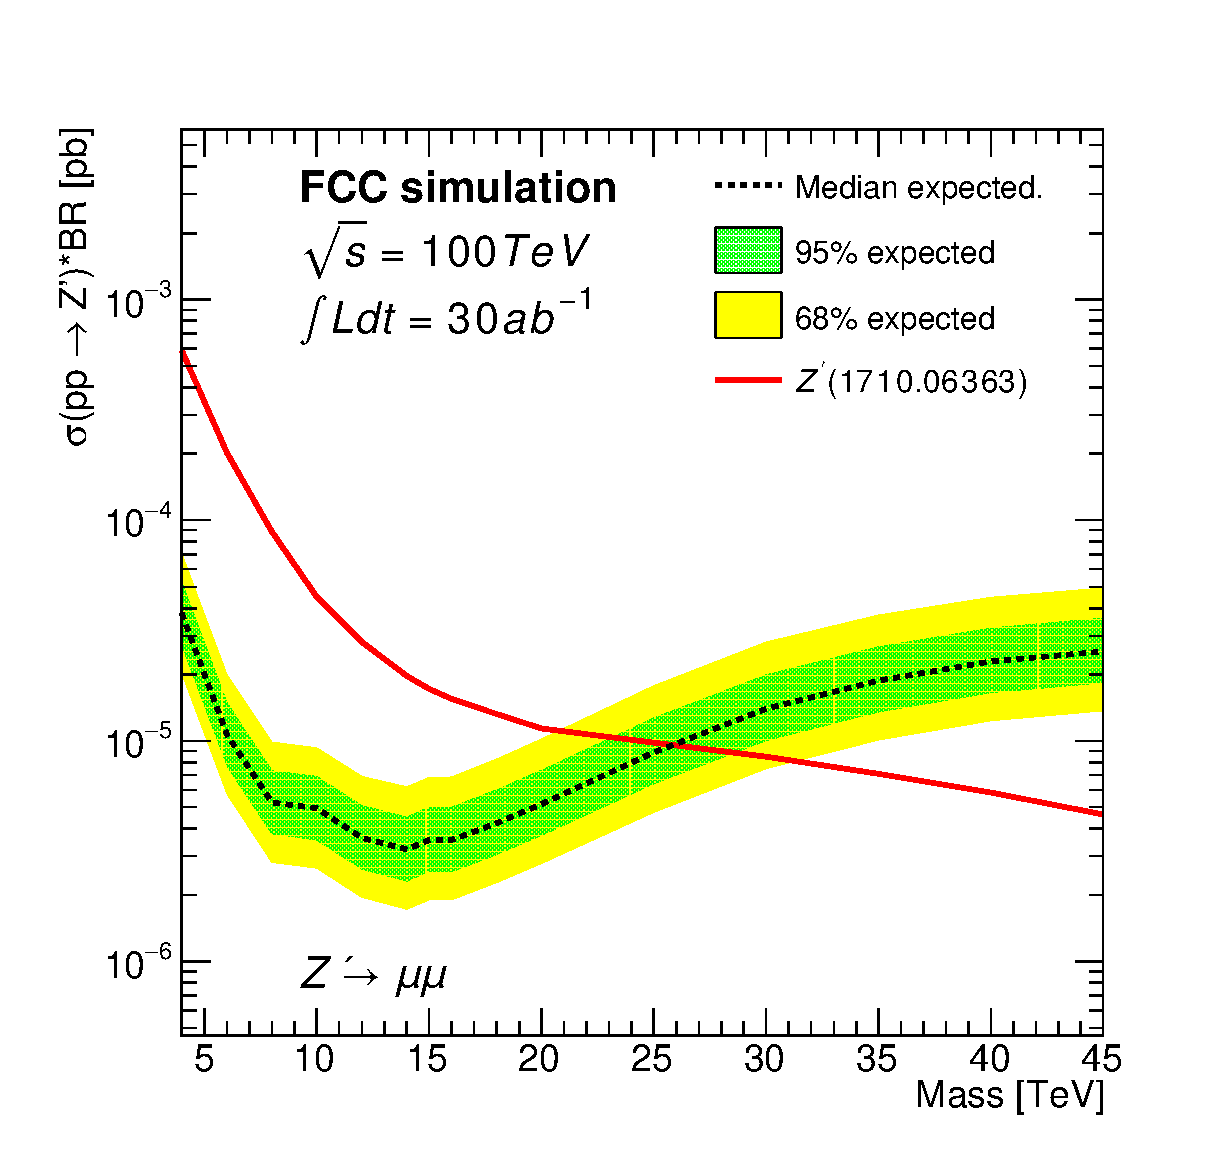
\includegraphics[width=0.32\columnwidth]{Fig/lim_Zprime_mumu_ano_fcc_v02.eps}
  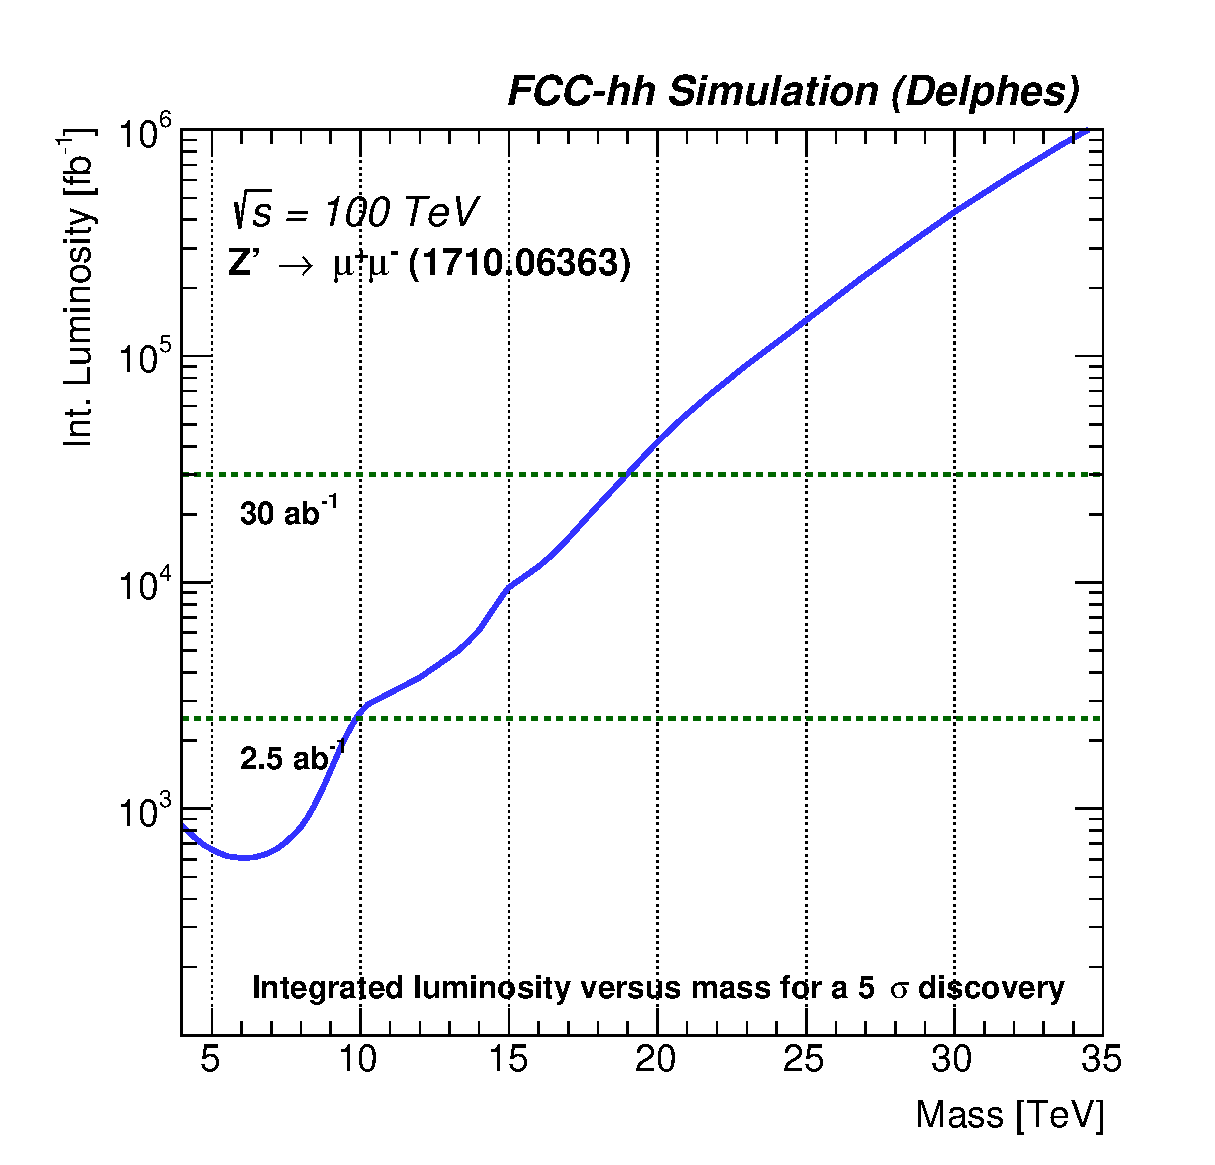
\includegraphics[width=0.32\columnwidth]{Fig/DiscoveryPotential_mumu_rootStyle.eps}
  \caption{Left : Invariant mass for a 30~TeV signal after full event selection in flavour anomaly scenario. Limit versus mass (middle) and luminosity for a $5\sigma$ discovery (right) comparing ee,$\mu\mu$ and combined channels. }
  \label{figure:leptonicresonances:resultsmumu_flav}
\end{figure}

\begin{figure}[!htb]
  \centering
  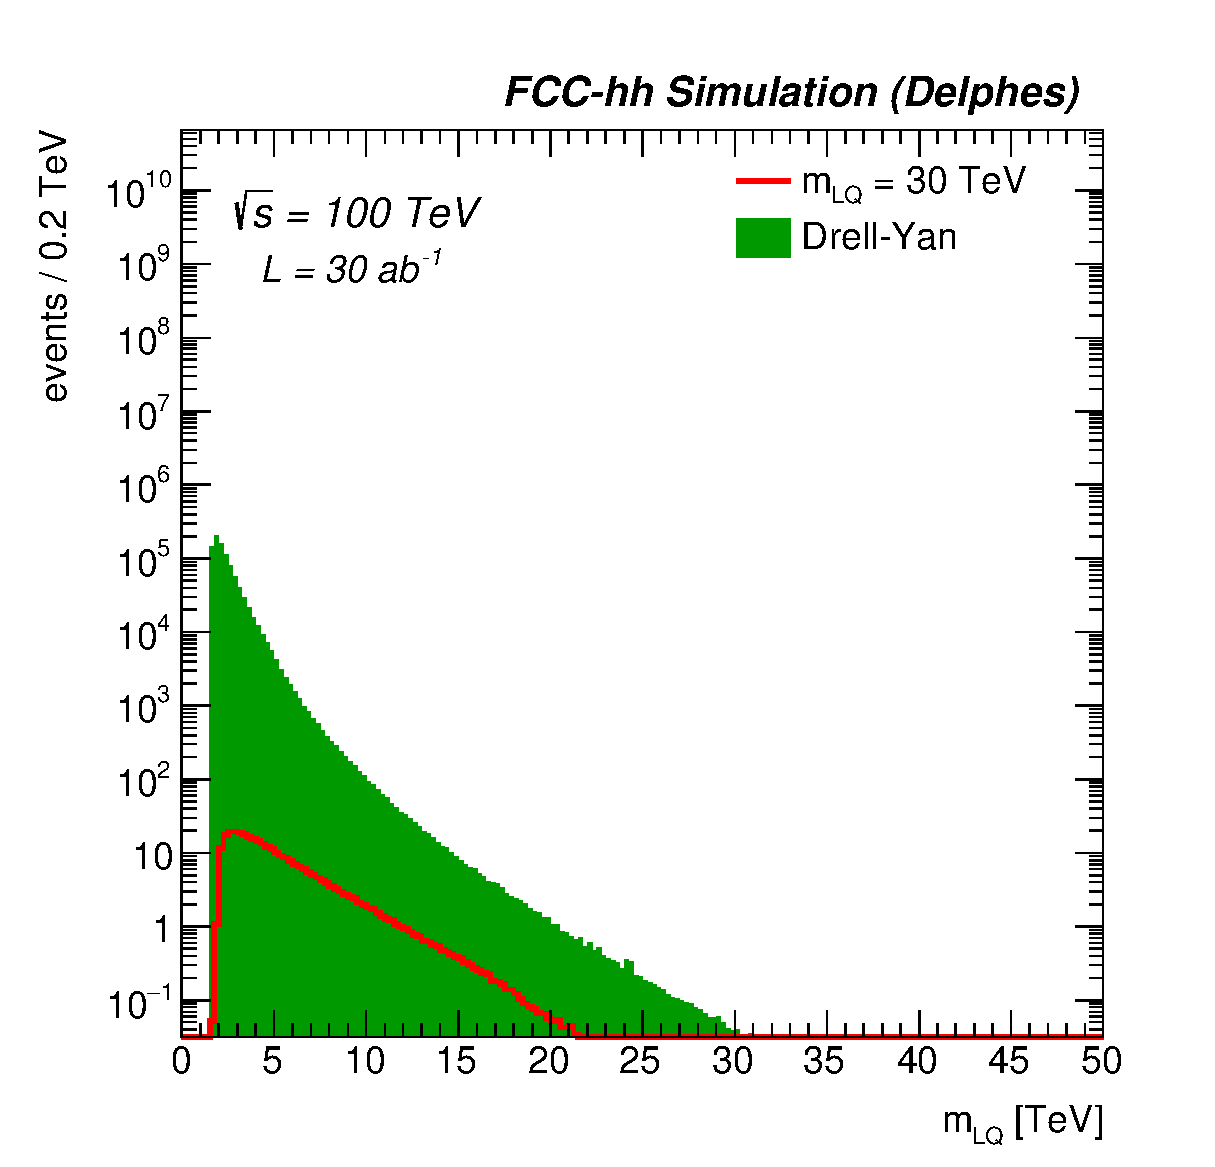
\includegraphics[width=0.32\columnwidth]{Fig/mlq_sel0_nostack_log.eps}
  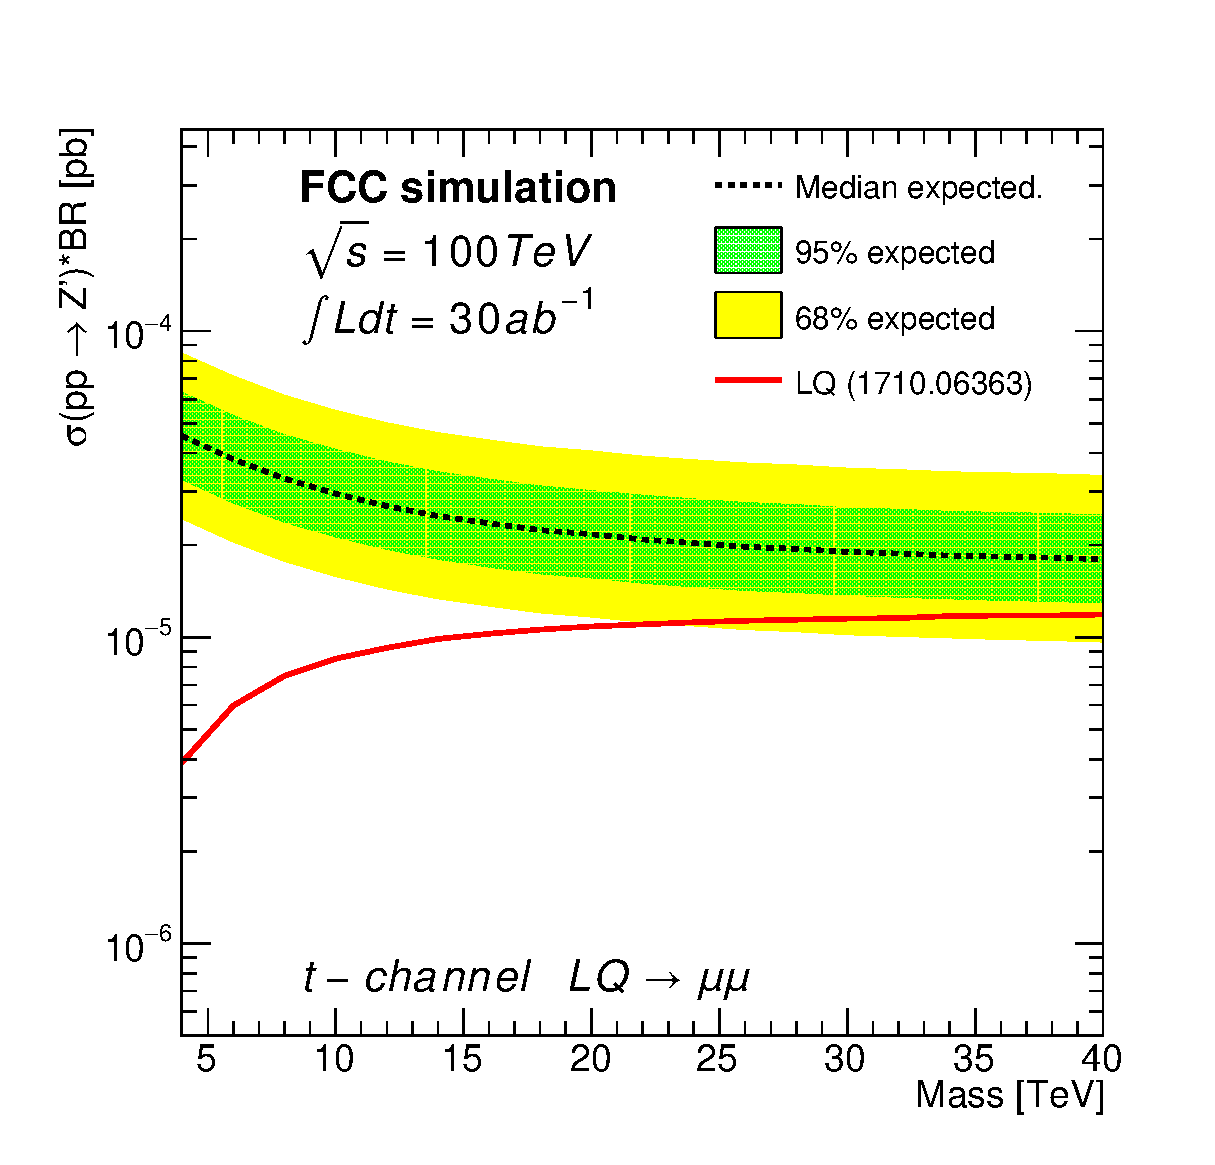
\includegraphics[width=0.32\columnwidth]{Fig/lim_LQ_mumu_fcc_v02.eps}
  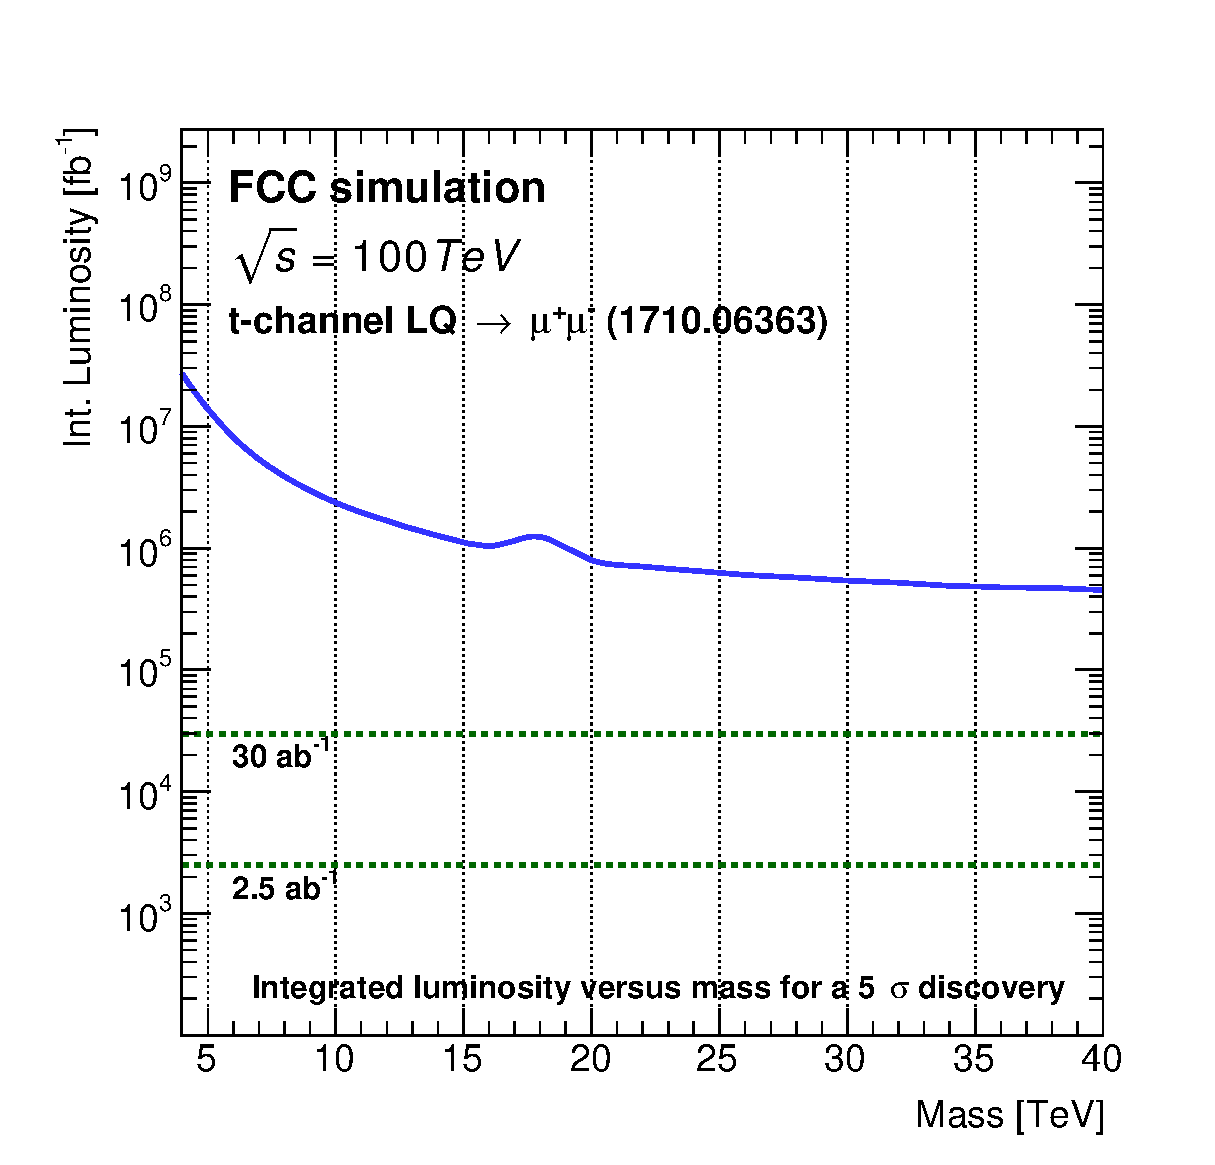
\includegraphics[width=0.32\columnwidth]{Fig/DiscoveryPotential_LQ_mumu_rootStyle.eps}
  \caption{Left : Invariant mass for a 30~TeV signal after full event selection in t-channel LQ scenario. Limit versus mass (middle) and luminosity for a $5\sigma$ discovery (right) comparing ee,$\mu\mu$ and combined channels. }
  \label{figure:leptonicresonances:resultsmumu_lq}
\end{figure}

\clearpage
\newpage

%%%%%%%%%%%%%%%%%%%%%%%%%%%%%%%%%%%%%%%%%%%%%%%%%%%%%
%%%%%%%%%%%%%%%%%%%%%%%%%%%%%%%%%%%%%%%%%%%%%%%%%%%%%
\subsection{Hadronic resonances : WW, \texorpdfstring{$t\bar{t}$}{tt}, jj}
\label{subsec:hadreso}

\subsubsection{Introduction}
Many models of beyond the SM (BSM) physics predict additional particles with masses at the TeV scale. The presence of new resonant states~\cite{Harris:2011bh,Boelaert:2009jm,Lee:1973iz,Branco:2011iw,Hill:1994hp,Kaplan:1983sm,Bellazzini:2014yua,Randall:1999ee,Pomarol:1999ad,Davoudiasl:1999tf} decaying to two highly boosted particles decaying hadronically could be observed as an excess in the QCD dijet distribution. We focus here on three specific benchmark models: a \ZpSSM~\cite{Langacker:2008yv}, a Randall-Sundrum graviton~\cite{Randall:1999ee}, and an excited quark resonance~\cite{Baur:1987ga,Baur:1989kv}. We study the sensitivity in the following decay using hadronic decay modes: \Zptt, \rsg\ and \qjj.

The decay products are typically in the multi-TeV regime and their reconstruction imposes stringent requirement on the detector design. Precise jet energy resolution requires full longitudinal shower containment. Highly boosted top quarks and $W$ bosons decay into highly collimated jets that need to  be disentangled from standard QCD jets by studying their substructure. High discrimination power and sensitivity for these searches at such extreme energies, requires excellent granularity both in the tracking detectors and calorimeters.

%%%%%%%%%%%%%%%%%%%%%%%%%%%%%%%%%%%%%%%%%%%%%%%%%%%%%%%%%%%%%%%%%%%%%%%%%%%%%%%%%%%%%%%%%%%%
\subsubsection{Event Selection}

\subparagraph{Dijet analysis}

Jets are clustered using particle-flow candidates with the anti-$k_T$~\cite{Cacciari:2008gp} algorithm with parameter R=0.4. We require at least two jets with $\pt$>3~TeV and $|\eta<3|$ and the rapidity difference between the two leading jets to be small, $\Delta(\eta)<1.5$ as di-jet events will tend to be more central. The dijet invariant mass of the \qjj\ signal for $m_Q^{*}$ and QCD contributions after the full event selection is shown in Figure~\ref{figure:hadronicresonances:ttsel08} (left).

\subparagraph{Boosted Top and W analyses}

As track jets are better able to resolve the jet sub-structure compared to particle-flow jets, the jet selection for the \rsg\ and \Zptt\ searches using track jets. As no lepton veto is applied, there is also some acceptance for leptonic decays. The sensitivity to semi-leptonic $WW$ or \ttbar\ decays is enhanced by adding the $\metvec$ vector to the closest jet 4-momentum (among the to leading jets).

We require two jets with a $\pt$>3~TeV and $|\eta<3|$ and $\Delta(\eta)<2.4$. Both jets must either be $W$ or top tagged (section~\ref{subsec:mvatagger}) by requiring multivariate tagger > 0.15. Both high-\pt\ jets must be $b$-tagged for the \Zptt\ analysis. Finally, to further reject QCD, we require for both jets $m_{SD}>40$~GeV. In Figure~\ref{figure:hadronicresonances:ttsel08} we show the di-jet invariant mass distribution after the final cuts for the \rsg\ (center) and \Zptt\ (right) analyses respectively.
\newline
More detailed results can be found in Appendix~\ref{appendix:zptt100} (\Zptt) and~\ref{appendix:rsg100} (\rsg).

\begin{figure}[!htb]
  \centering
  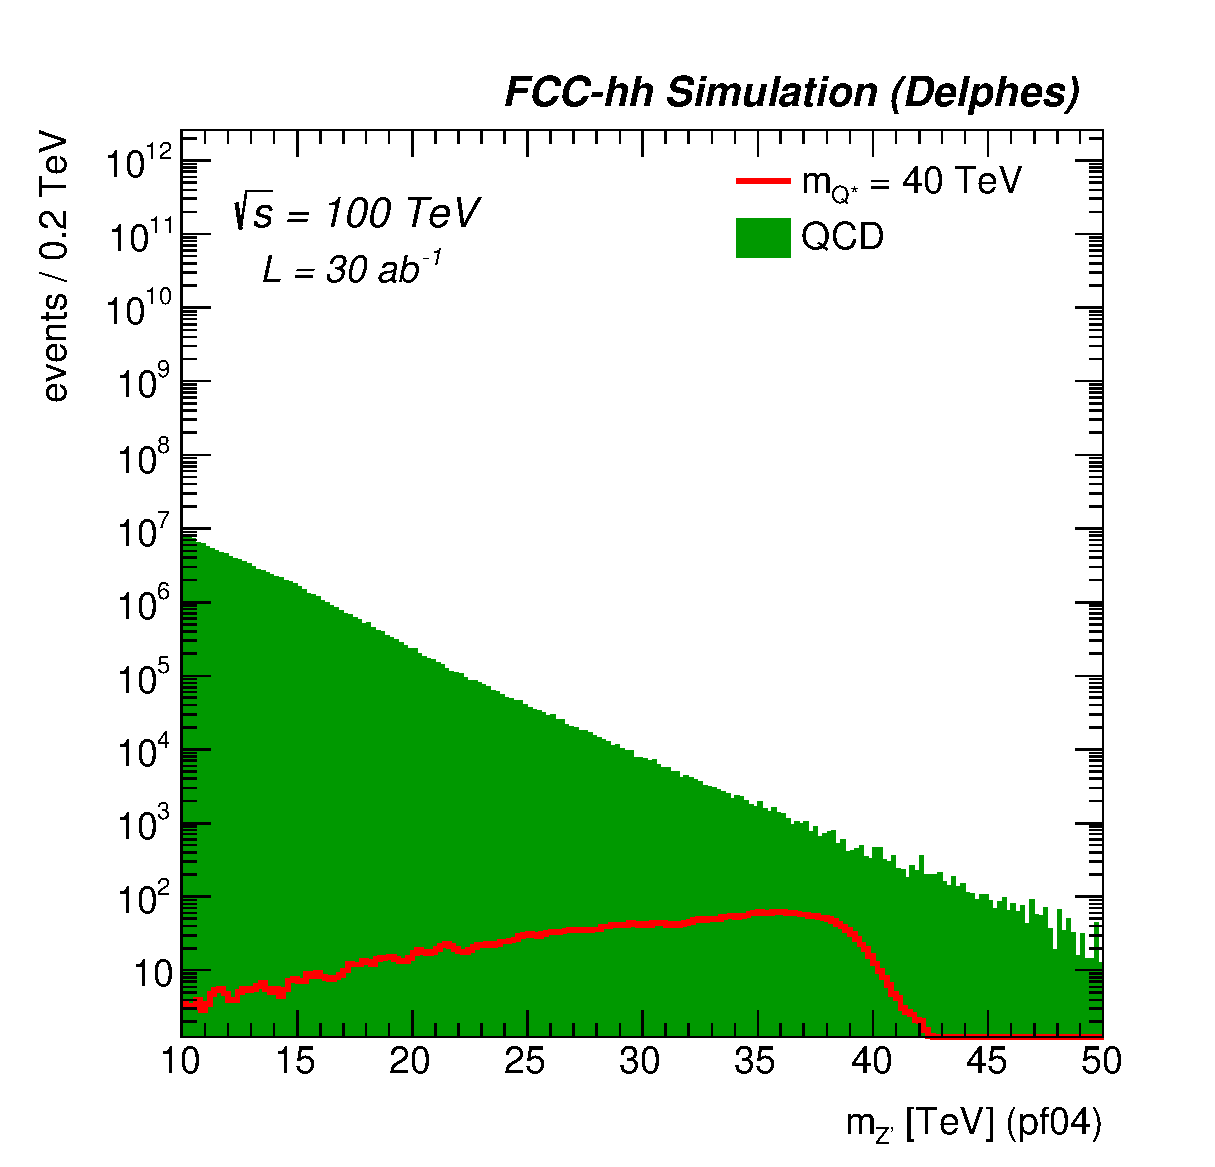
\includegraphics[width=0.32\columnwidth]{Fig/Mj1j2_pf04_sel1_nostack_log.eps}
  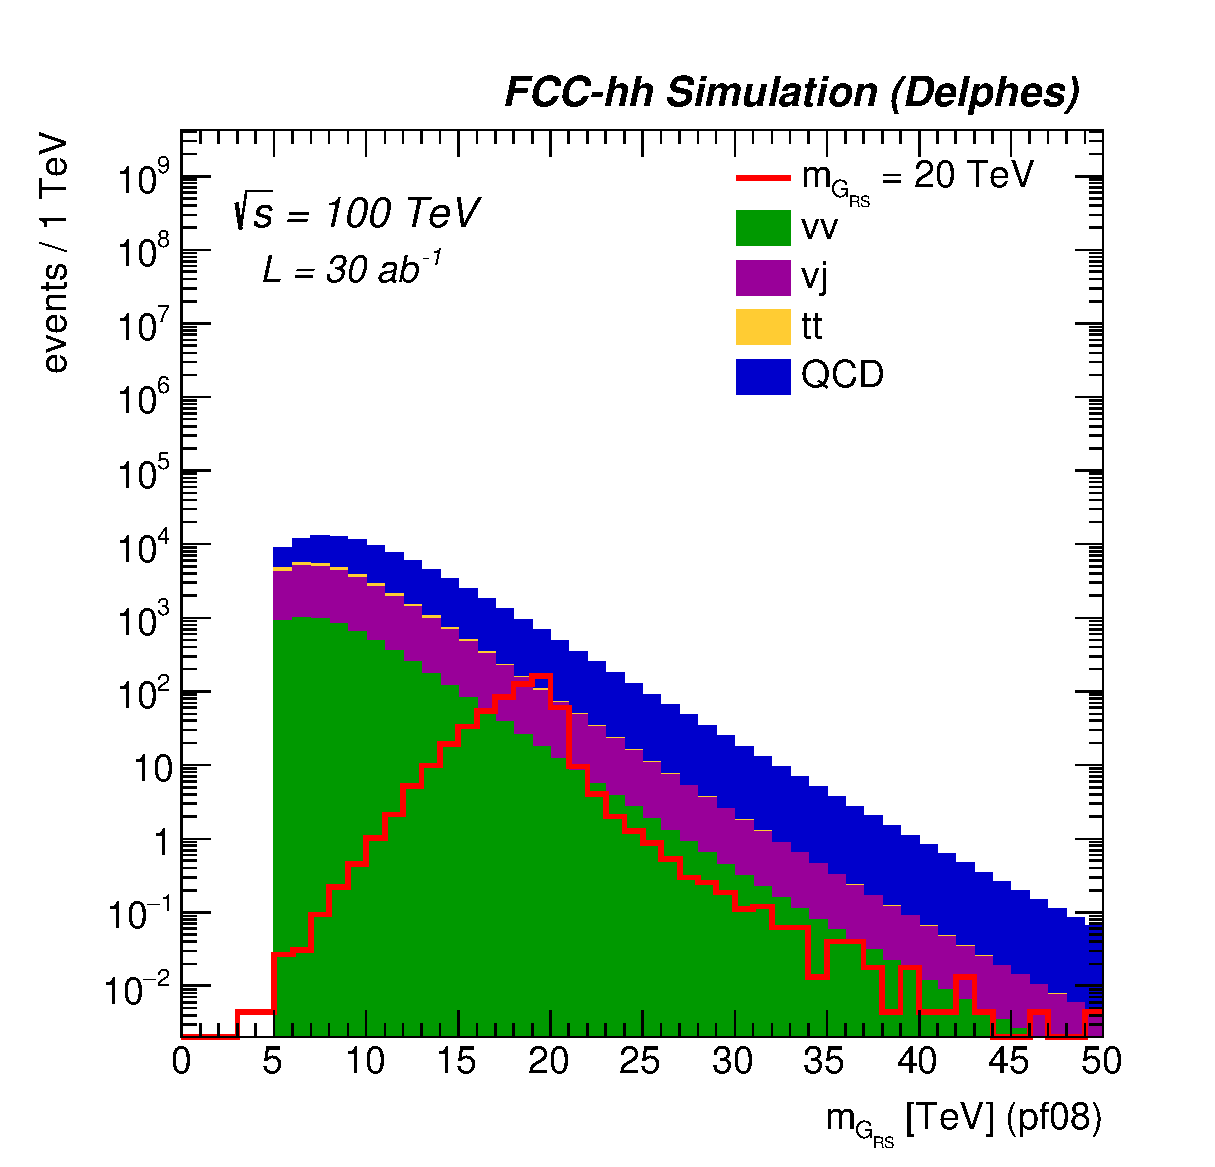
\includegraphics[width=0.32\columnwidth]{Fig/Mj1j2_pf08_fit_sel4_nostack_log.eps}
  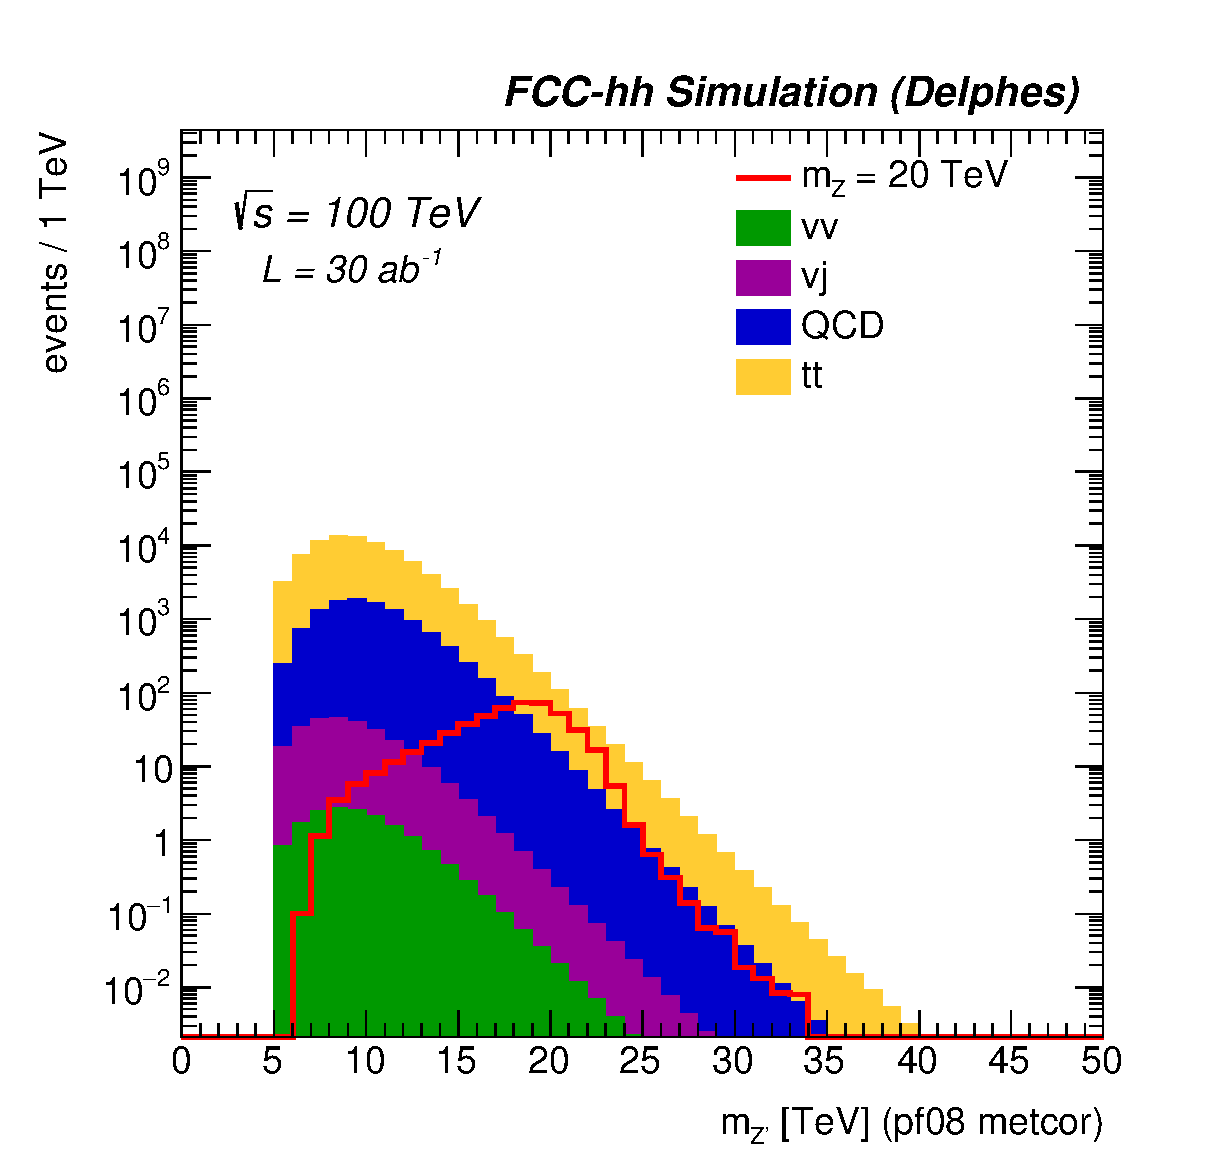
\includegraphics[width=0.32\columnwidth]{Fig/Mj1j2_pf08_MetCorr_fit_sel8_nostack_log.eps}
  \caption{Invariant mass distribution of the two leading jets for the pre-selection (left) and full selection (right) for a 40~TeV signal for the \qjj\ (left), and a 20~TeV signal for \rsg\ (center) and \Zptt\ (right) analyses.\MS{need editing / style}}
  \label{figure:hadronicresonances:ttsel08}
\end{figure}

\begin{table}[htbp]
   \centering
\begin{tabular}{|c|c|c|c|c|c|c|c|c|}
  \hline
  \hline
  & \multicolumn{2}{c|}{di-jet}  & \multicolumn{2}{c|}{$\ttbar$} & \multicolumn{2}{c|}{WW} \\
  \cline{2-7}

 & pre-sel & final-sel  & pre-sel & final-sel & pre-sel & final-sel\\
  \hline
  di-jet & 385555434 &  373661126 &  154855591 & 11439.8&  154856148 & 64484\\
  $\ttbar$ & - & - & 1114779 & 74193.6 &  1114779 & 3185\\
  di-bosons & - & - &  41820 &  17.1 &  41820 & 6092\\
  boson+jet & - & - & 1610472 & 264.1&  1610472 & 25377\\
  \hline
  total bkg  &  385555434& 373661126& 157622662 & 85914 & 154856148 & 99137\\
  \hline
  10~TeV &  - & - &  101529 & 15601 &  47853 & 15745\\
  20~TeV &   1253072 &  1239813& 7774 & 500.6 & 1282 & 578\\
  30~TeV &  69922 &  67488 & 485.2 & 13.2 &  61.4 & 30.1 \\
  40~TeV &  4589 &  4373 & - & - & - & -\\
  \hline
  \hline
\end{tabular}
  \caption{Yields for the di-jet, $\ttbar$ and WW analyses after pre and final selection.}
  \label{tab:hadronicresonances:yields}
\end{table}

%%%%%%%%%%%%%%%%%%%%%%%%%%%%%%%%%%%%%%%%%%%%%%%%%%%%%%%%%%%%%%%%%%%%%%%%%%%%%%%%%%%%%%%%%%%%
\subsubsection{Signal extraction and results}
Hypothesis testing is performed using a modified frequentist method based on a profile likelihood fit that takes into account the systematic uncertainties as nuisance parameters. The di-jet invariant mass is used as a discriminant. In order to reduce large statistical fluctuations from high Monte Carlo weight events, we parameterize the background invariant mass distribution with the following function (conservatively assuming 50\% uncertainty on the background normalisation) $f(z)=p_1(1-z)^{p_2}z^{p_3}z^{p_{4}logz}$, where $z=m_{jj}/\sqrt{s}$.

The expected exclusion limits at 95\% CL are shown in Figures~\ref{figure:hadronicresonances:limits} and~\ref{figure:hadronicresonances:resultsjj}. For the \qjj\ masses up to 40~TeV could be discovered with \intlumifcc. Reconstructing Heavy resonances decaying to $WW$ and \ttbar\ is more challenging and requires the use of novel approaches to boosted object tagging to reduce the backgrounds. The reach for \Zptt\ (in TC2 models) and \rsg\ is 24~TeV and 22~TeV respectively and it is possible to discover a $Z^{\prime}_{SSM} \rightarrow \ttbar$ up to $m_{Z}=18$~TeV.

\begin{figure}[!htb]
  \centering
  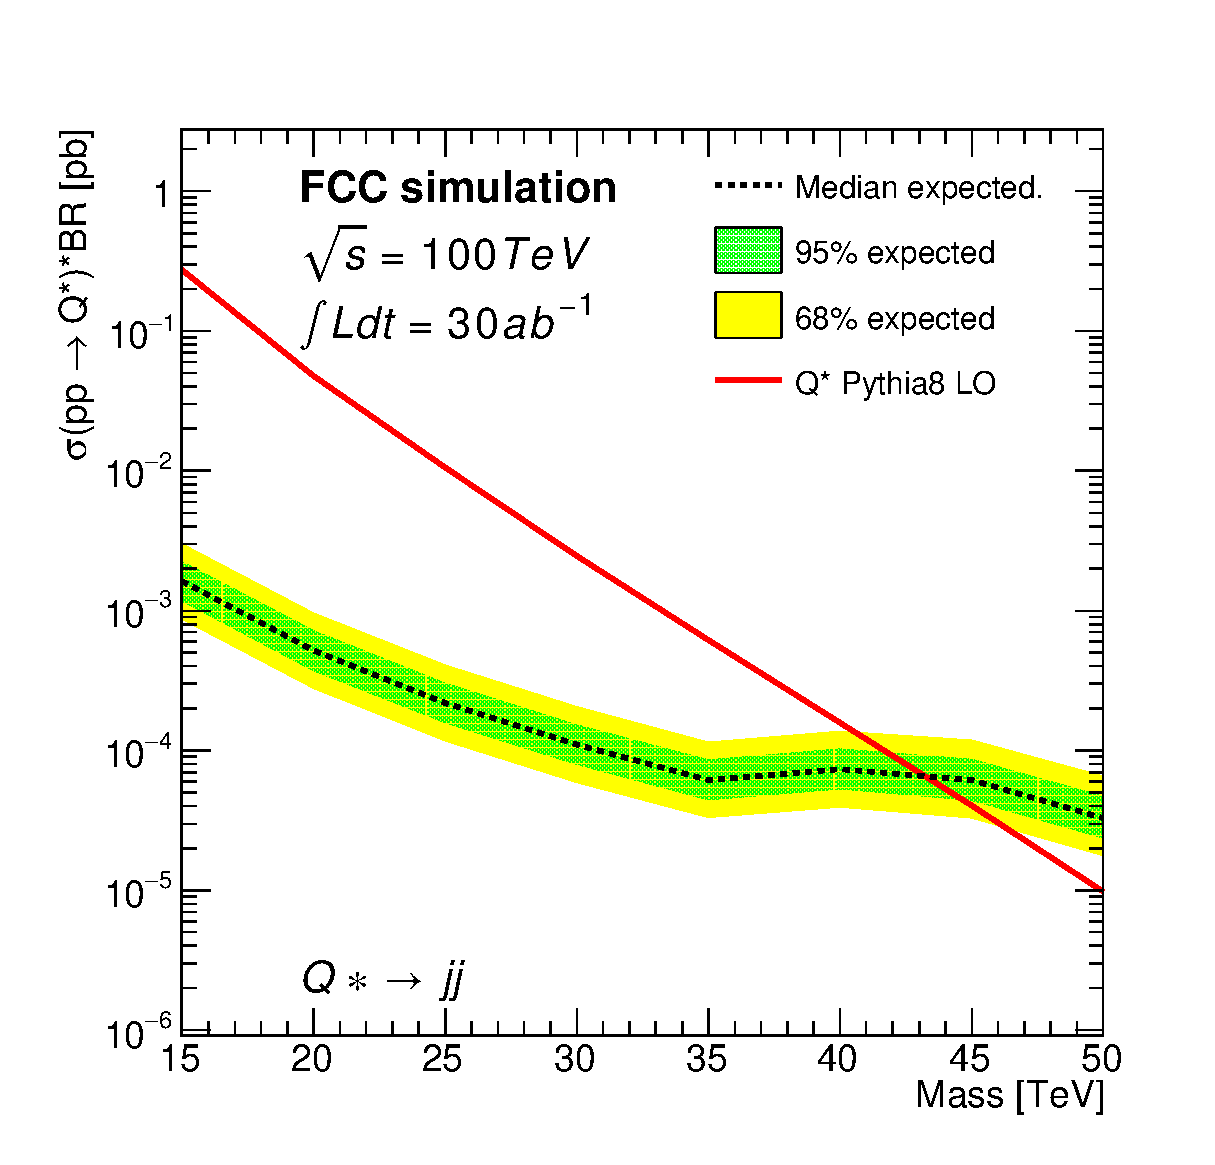
\includegraphics[width=0.30\columnwidth]{Fig/lim_Qstar_jj_fcc_v02.eps}
  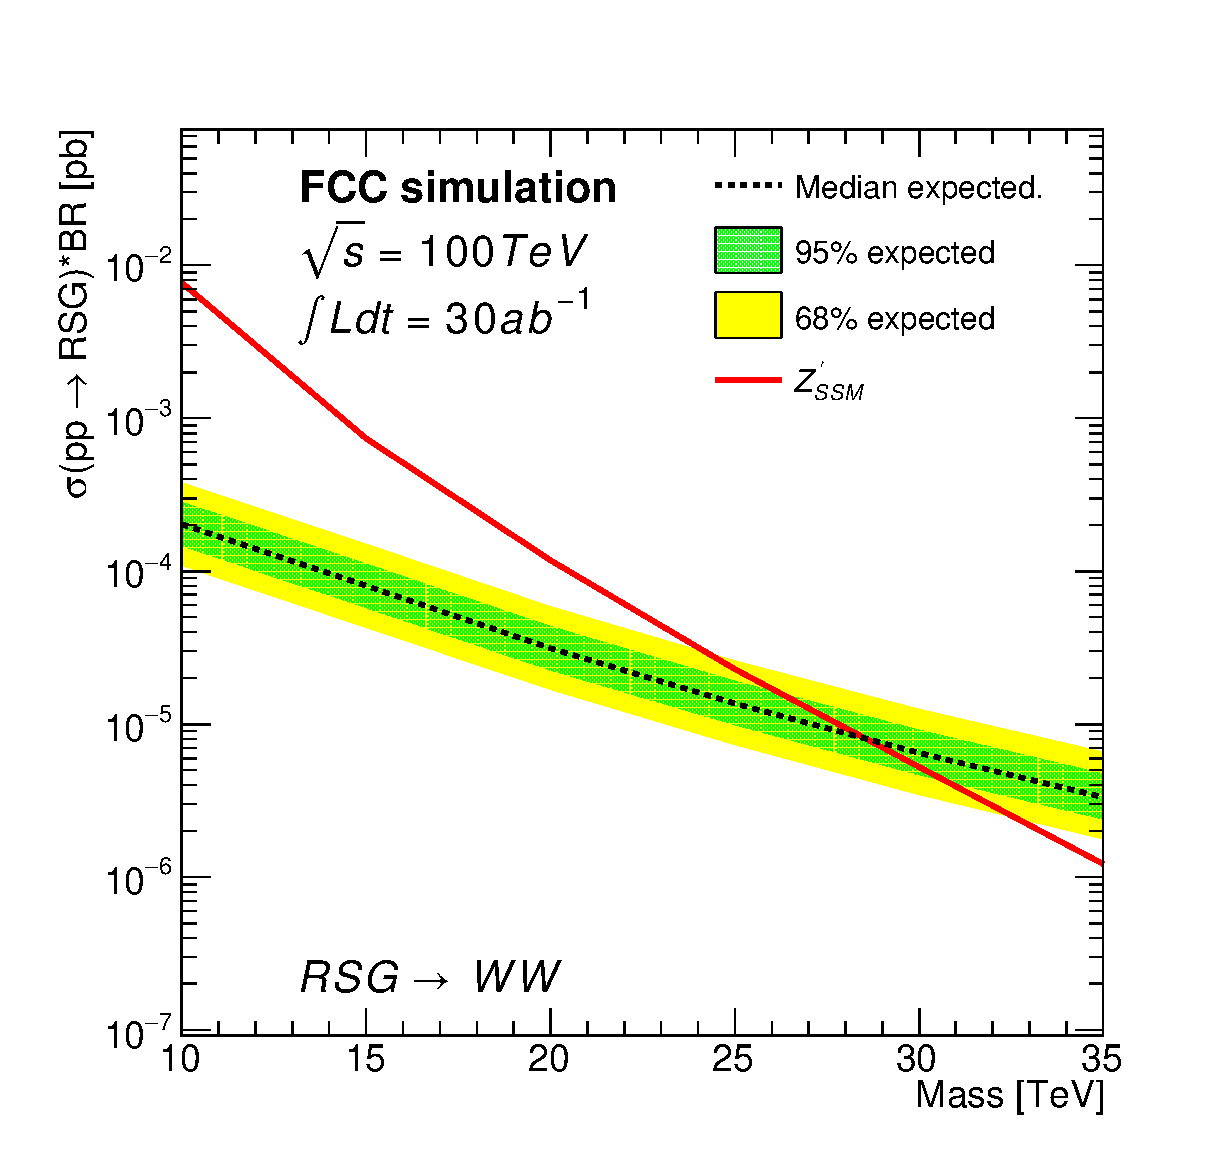
\includegraphics[width=0.30\columnwidth]{Fig/lim_RSGraviton_ww_fcc_v02.eps}
  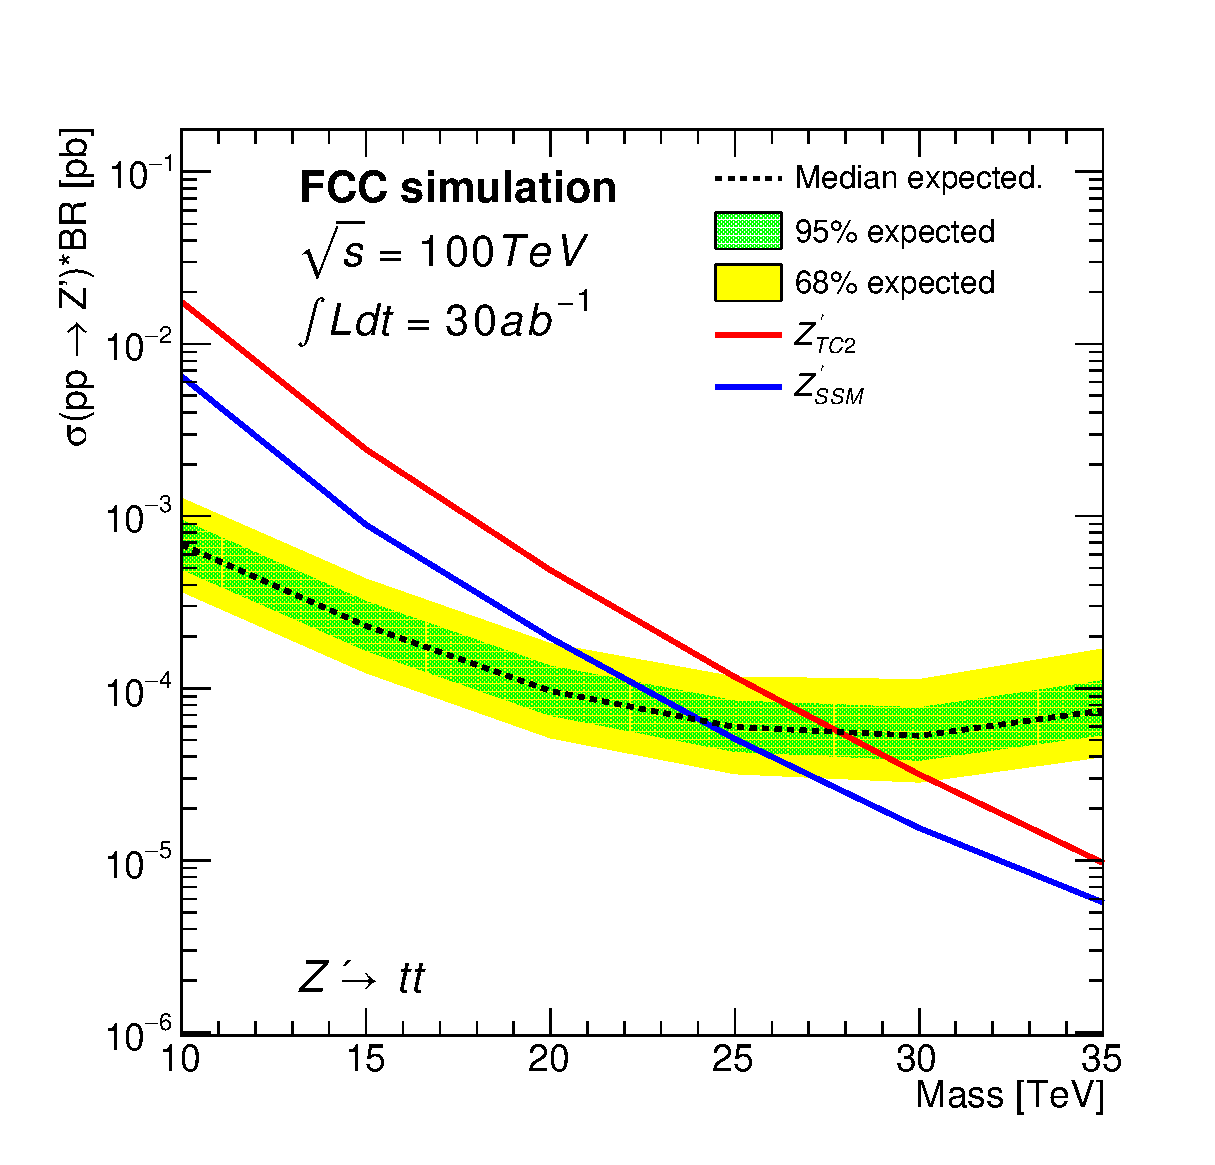
\includegraphics[width=0.30\columnwidth]{Fig/lim_Zprime_tt_fcc_v02.eps}
  \caption{Exclusion limit at 95\% CL versus heavy resonance mass decaying into di-jet (left), WW (center), \ttbar\ (right).}
  \label{figure:hadronicresonances:limits}
\end{figure}

\begin{figure}[!htb]
  \centering
  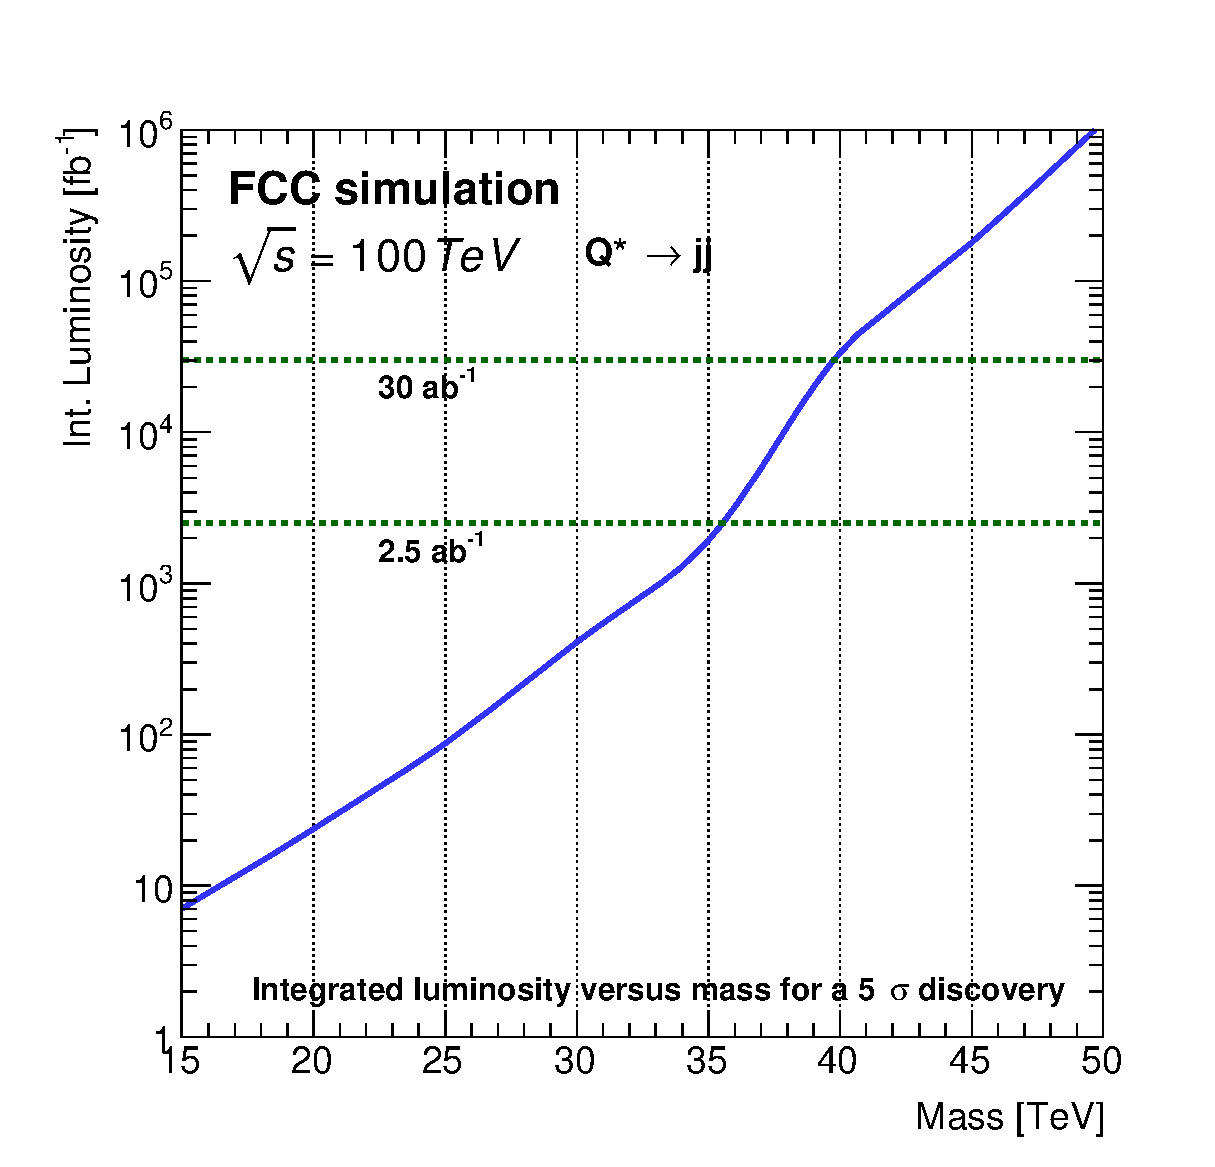
\includegraphics[width=0.30\columnwidth]{Fig/DiscoveryPotential_jj_rootStyle.eps}
  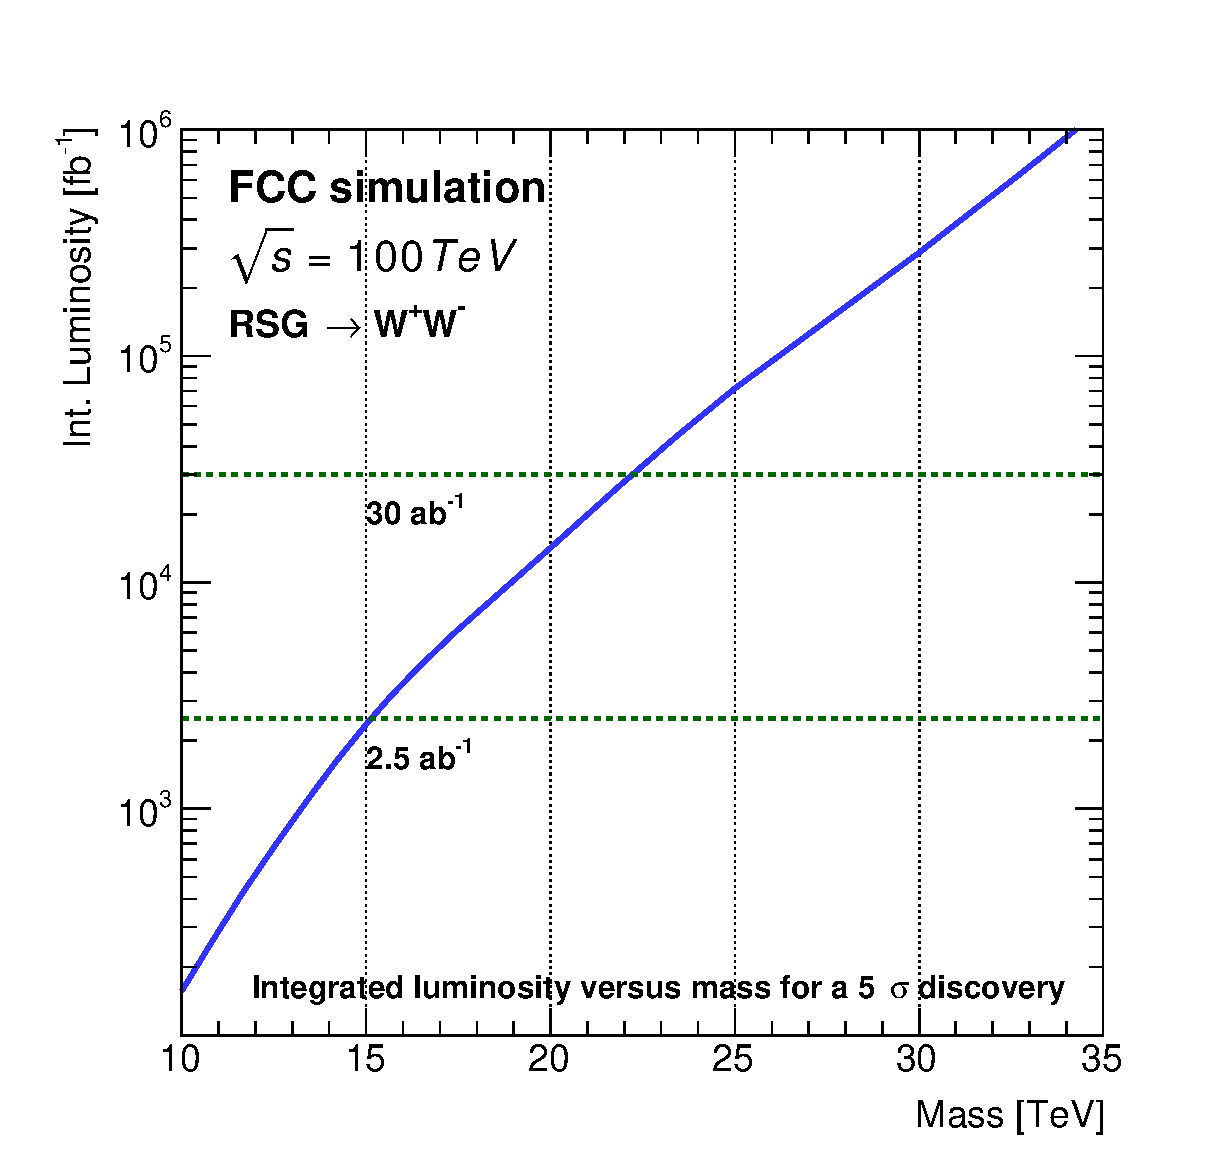
\includegraphics[width=0.30\columnwidth]{Fig/DiscoveryPotential_ww_tagger_rootStyle.eps}
  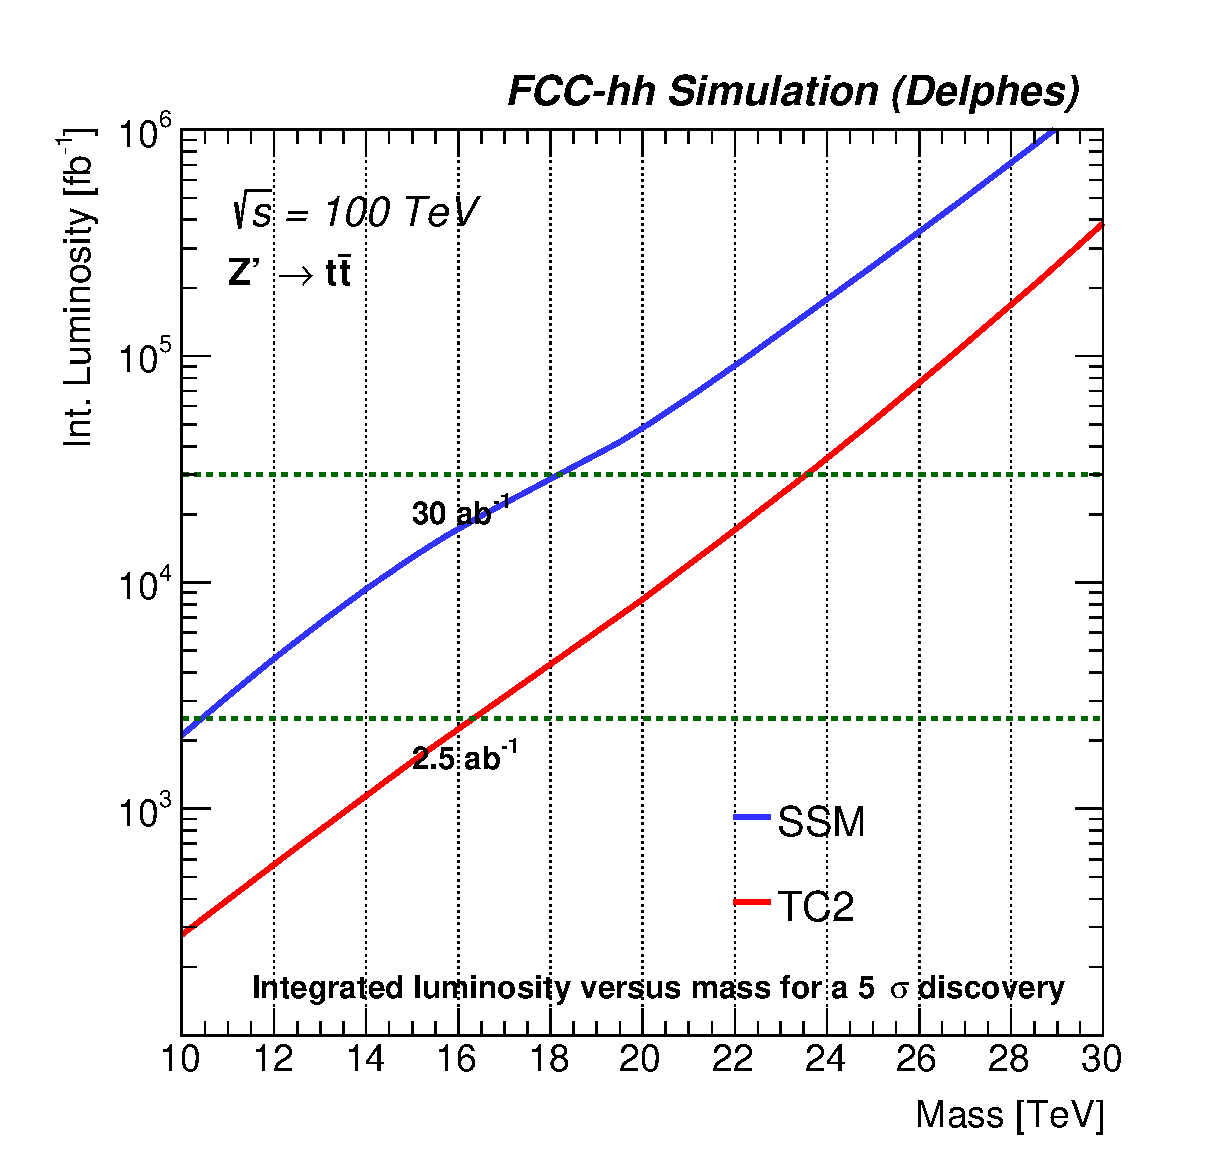
\includegraphics[width=0.30\columnwidth]{Fig/DiscoveryPotential_tt_SSM_TC2_tagger_TRFbtag_rootStyle.eps}
  \caption{Integrated luminosity for a $5\sigma$ discovery as a function of the heavy resonance mass decaying into di-jet (left), WW (center), \ttbar\ (right).}
  \label{figure:hadronicresonances:resultsjj}
\end{figure}

%%%%%%%%%%%%%%%%%%%%%%%%%%%%%%%%%%%%%%%%%%%%%%%%%%%%%
%%%%%%%%%%%%%%%%%%%%%%%%%%%%%%%%%%%%%%%%%%%%%%%%%%%%%
\subsection{Summary}
\label{subsec:summary100tev}

The discovery potential for resonances considered in FCC-hh scenario are summarised in Figure~\ref{figure:resonances100:summary}.

\begin{figure}[!htb]
  \centering
  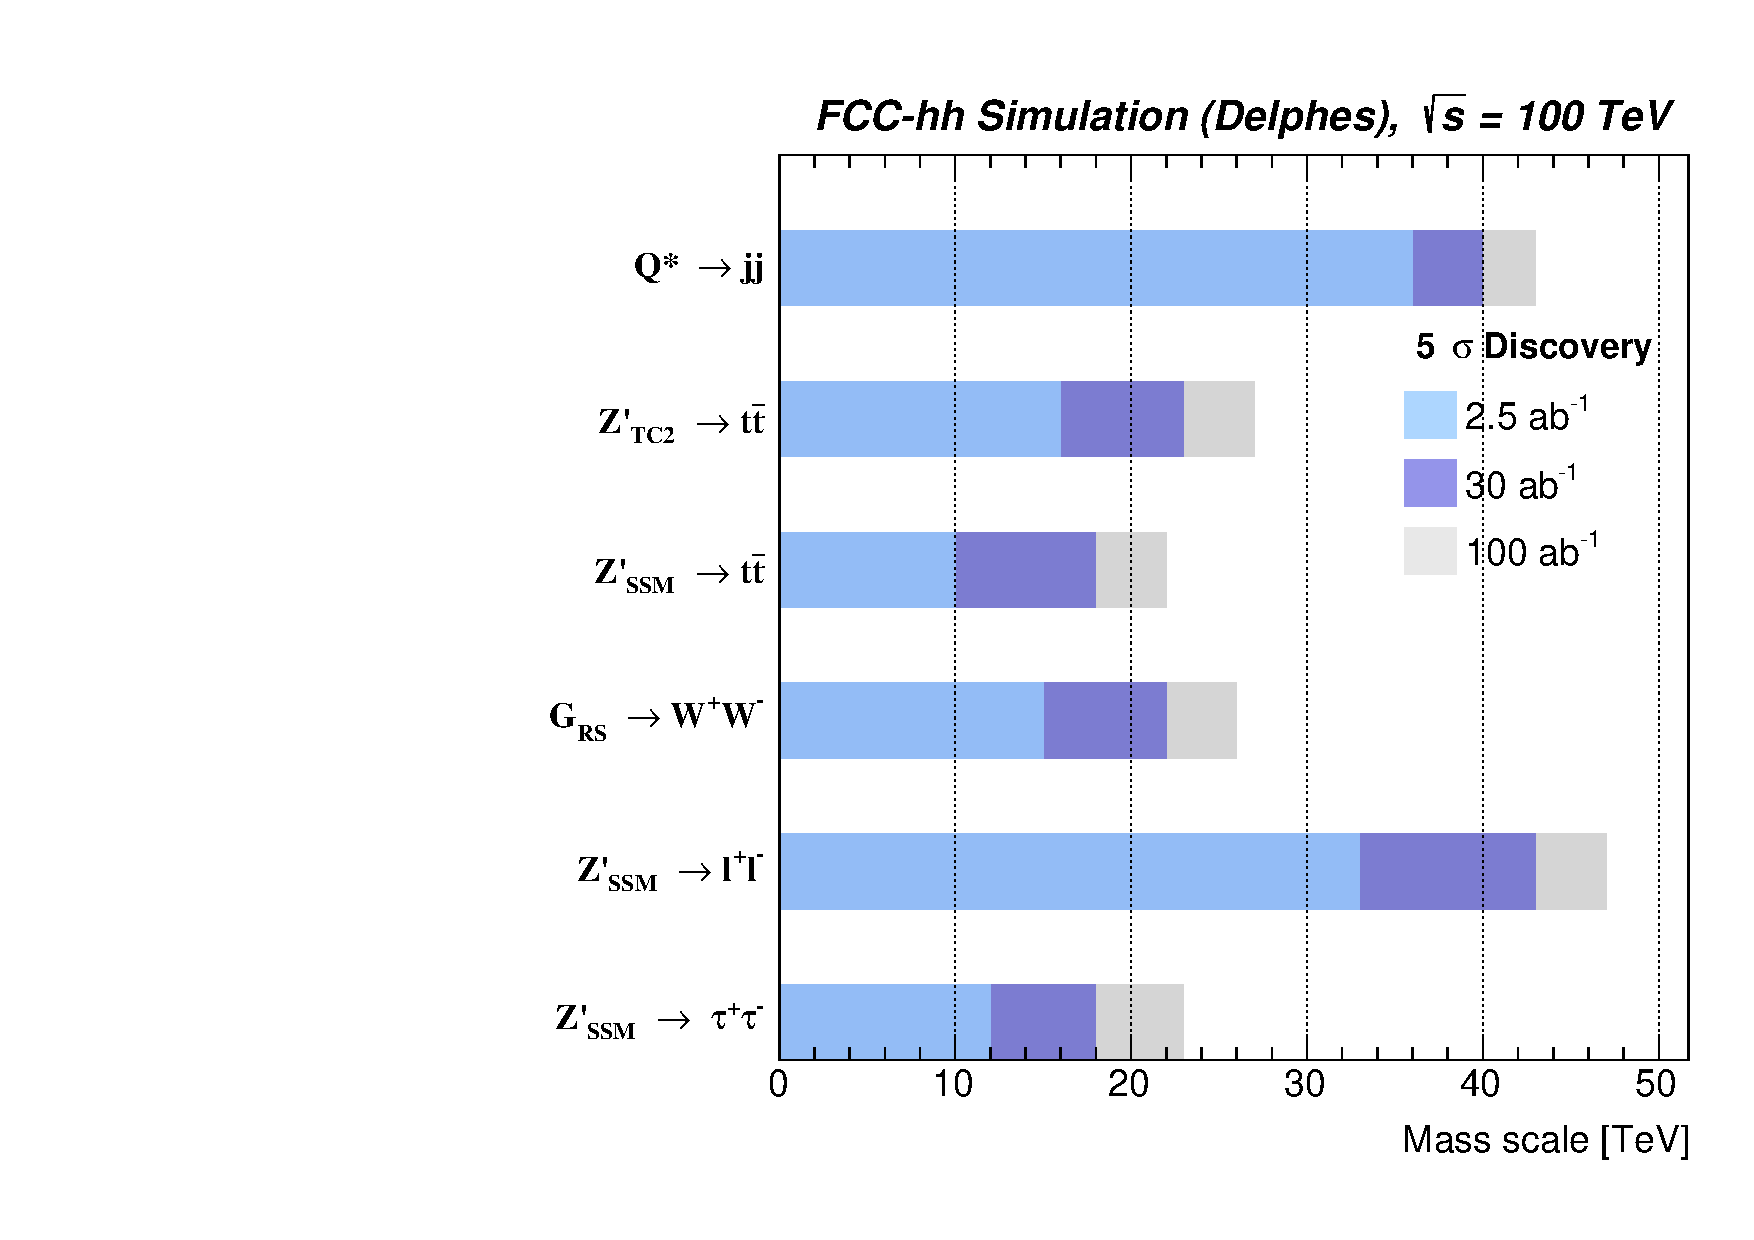
\includegraphics[width=0.90\columnwidth]{Fig/summaryDisco_onlyFCChh.pdf}
  \caption{Summary of a $5\sigma$ discovery reach as a function of the resonance mass for different luminosity scenario of FCC-hh.}
  \label{figure:resonances100:summary}
\end{figure}

\clearpage
\newpage

%%%%%%%%%%%%%%%%%%%%%%%%%%%%%%%%%%%%%%%%%%%%%%%%%%%%%
\section{Comparison with 27 TeV HE-HLC}
\label{sec:ana27tev}
A comparison with HE-LHC scenario has been performed.
In order to achieve it all the samples have been rederived with the associated expected energy of 27 TeV and the benchmark luminositiy used is 15 $a^{-1}$ .
\newline
The analyses strategies are the same, only the thresholds have been updated for the 27 TeV conditions. Here is the detail of the changes done :
\begin{itemize}
\item \Zpee\ or \Zpmumu : leton $p_T$ lowered from 1TeV to 0.5 TeV,
\item \Zpmumu\ f.a. and t-channel LQ : leton $p_T$ lowered from  1.2 TeV to 0.75 TeV,
\item \Zptata\ : optimal cuts changed as shown in Table~\ref{tab:leptonicresonances:selectiontautau27},
\item \rsg\ : $Jet^{trk02}(p_T^{SD Corr})$ lowered from 3 TeV to 1 TeV,
\item \Zptt\ : $Jet^{trk02}(p_T^{SD Corr})$ lowered from 3 TeV to 1 TeV,
\item \qjj\ : $Jet^{calo04}(p_T)$ lowered from 3 TeV to 1 TeV.
\end{itemize}

Table~\ref{tab:27vs100} shows the detailed results of the limit and discovery reach at $5\sigma$ for the HE-LHC 27 TeV and FCC-hh 100 TeV scenarios.
The discovery potential comparison can be found in Figure~\ref{figure:resonances27comp100:summary}.
More detailed results can be found for each 27 TeV analysis in Appendix~\ref{appendix:zpll27},~\ref{appendix:zpmumufalvano27},~\ref{appendix:zptautau27},~\ref{appendix:zptt27},~\ref{appendix:rsgww27}  and~\ref{appendix:qstarjj27}.

\begin{table}[htbp]
   \centering
\begin{tabular}{|l|l|c|r|}
  \hline
  \hline
   $\Zp$ mass [TeV] &  $\Delta \phi(\tau_1, \tau_2)$&  $\Delta R(\tau_1, \tau_2)$ & $\met$\\
  \hline
   $2$ & > 2.4 & > 2.4 and < 3.9 & > 80 GeV\\
   $4$ & > 2.4 & > 2.7 and < 4.4 & > 80 GeV\\
   $6$ & > 2.4 & > 2.9 and < 4.4 & > 80 GeV\\
   $8$ & > 2.6 & > 2.9 and < 4.6 & > 80 GeV\\
  $10$ & > 2.8 & > 2.9 and < 4.1 & > 60 GeV\\
  $12$ & > 2.8 & > 3.0 and < 3.6 & > 60 GeV\\
  $14$ & > 3.0 & > 3.0 and < 3.3 & > 60 GeV\\
  \hline
  \hline
  \end{tabular}
  \caption{List of mass dependent cuts optimised to maximise the sensitivity for the \Zptata\ search.}
  \label{tab:leptonicresonances:selectiontautau27}
\end{table}

\begin{table}[!htb]\centering
\begin{tabular}{|c|c|c|c|}
\hline
\hline
analysis   & \multicolumn{3}{c|}{HE-LHC (FCC-hh)} \\
           & Limit [TeV] & Disco [TeV]   & Disco [TeV] \\
           &             & 1 (2.5) $ab^{-1}$ & 15 (30) $ab^{-1}$ \\
\hline
\Zpee+\Zpmumu & 13 (40) & 10 (33) & 13 (43) \\
\Zptata       &  6 (14) &  3 (12) &  6 (18) \\
\Zpmumu\ f.a. &  4 (25) &  - (10) &  2 (19) \\
\Zptt         & 10 (28) &  6 (16) &  8 (23) \\
\rsg          &  8 (28) &  5 (15) &  7 (22) \\
\qjj          & 14 (43) & 10 (36) & 12 (40) \\
\hline
\hline
\end{tabular}
\caption{Limit and discovery reach at 5 $\sigma$ comparison between HE-LHC (27 TeV 15 ab-1) and FCC-hh (100 TeV 30 ab-1).}
\label{tab:27vs100}
\end{table}

\begin{figure}[!htb]
  \centering
  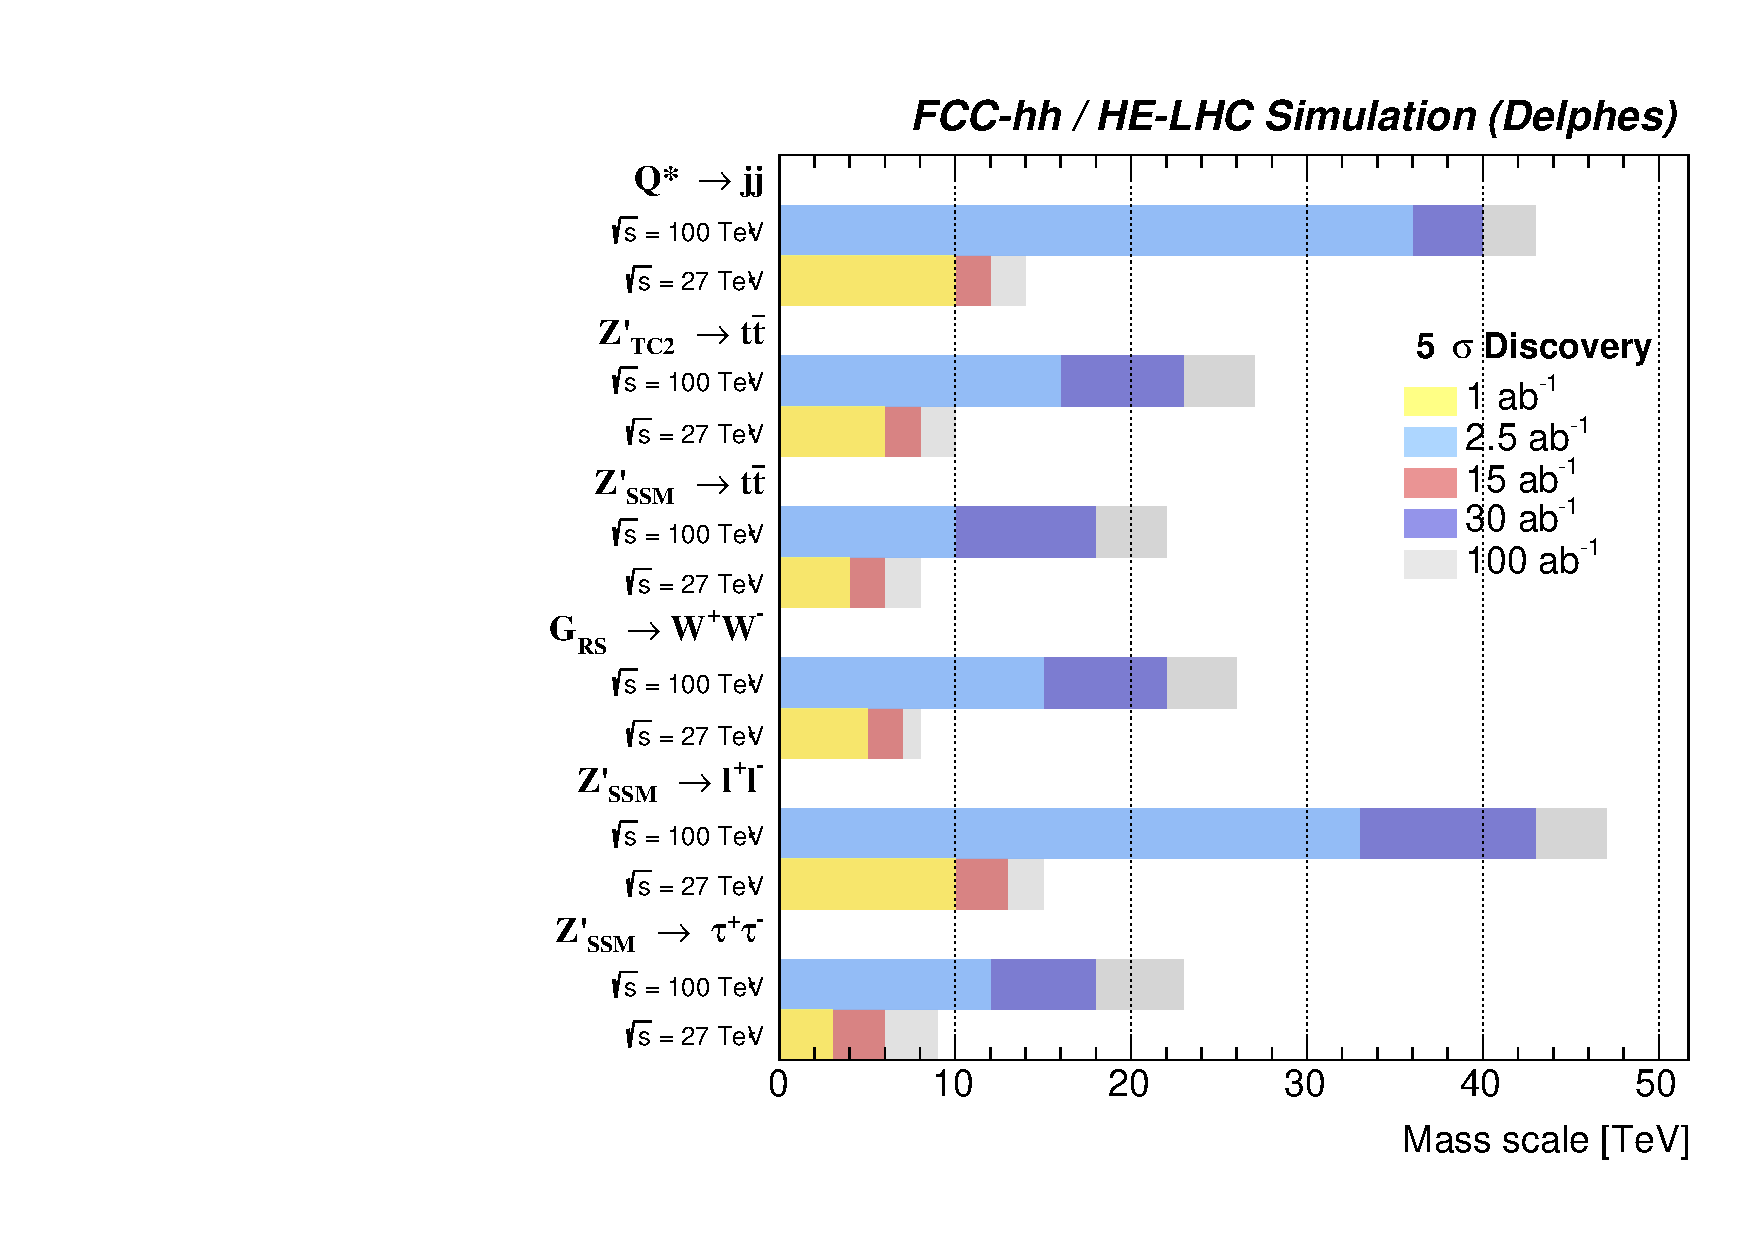
\includegraphics[width=0.90\columnwidth]{Fig/summaryDisco.pdf}
  \caption{Summary of a $5\sigma$ discovery reach as a function of the resonance mass for different luminosity scenario of FCC-hh and HE-LHC.}
  \label{figure:resonances27comp100:summary}
\end{figure}
\section{Model discrimination at HE-LHC}
The 14 TeV LHC with L=3 ab$^{-1}$ of integrated luminosity can search for new $Z'$ gauge bosons from the classic extended gauge theories up to masses 
of roughly $\simeq 6$ TeV.  Here we analyzed the capability of the 27 TeV HE-LHC with L=15 ab$^{-1}$ to distinguish among six $Z'$ models employing for the leptonic decays only 
the $e^+e^-$ and $\mu^+\mu^-$ channels, and top b and light jets for the hadronic decays and assuming that $M_{Z'}=6$ TeV. Under the assumption that these $Z'$'s decay only to SM particles,  we show that 
there are sufficient observables to perform this model differentiation in most cases. 

%%%%%%%%%%%%%%%%%%%%%%%%%%%%%%%%%%%%%%%%%%%%%%%%%%%%%
\subsection{Context of the study}
It is legitimate to assume that a heavy resonance could be seen at the end of High Luminosity LHC (HL-HLC). If that is the case a new collider with higher energy 
in the center of mass is needed to study its property as not enough events will be available at 14~TeV. In this document we present the discrimination potential of a High Energy LHC (HE-LHC)
with an assumed center of mass energy of 27~TeV.


%%%%%%%%%%%%%%%%%%%%%%%%%%%%%%%%%%%%%%%%%%%%%%%%%%%%%
\subsection{Bounds from HL-LHC}
As a starting point it is needed to understand what are, for $\sqrt s=14$ TeV, for the typical exclusion/discovery reaches for some standard reference $Z'$ models assuming L=3 ab$^{-1}$ 
employing only the $e^+e^-$ and $\mu^+\mu^-$ channels. To address this and the other questions below we will use the same set of $Z'$ models as employed 
in \cite{Rizzo:2014xma} and mostly in \cite{Han:2013mra}, both of which we will refer to frequently. We employ the MMHT2014 NNLO set \cite{Harland-Lang:2014zoa} 
throughout with an appropriate constant $K$-factor (=1.27) for numerics. 
The upper panel in Fig.~\ref{toy} shows the production cross section times leptonic BF for these models at 14 TeV in the NWA. It has 
been and will be assumed here that these $Z'$ states only decay to SM particles. 

Using the present ATLAS and CMS results at 13 TeV, \cite{Aaboud:2017buh} and \cite{Sirunyan:2018exx}, it is straightforward to estimate by extrapolation the eventual 14 TeV 
exclusion reach in the combined $e+\mu$ sample; this is given in the first column of Table~\ref{spec}. For discovery, only the $e$ channel is used due to poor $\mu$-pair mass 
resolution near $M_{Z'}=6$ TeV although the muons will add some additional support for any observed excess as large masses. Estimates of the $3\sigma$ evidence and $5\sigma$ 
discovery limits are also given in the Table. Based on these results, we will assume in our study below that we are dealing with a $Z'$ of mass 6 TeV; somewhat smaller mass 
choices will lead to very similar conclusions based on the ratio of predicted event rates shown in the lower panel of Fig.~\ref{toy}.  Fig.\ref{toy2} shows the NWA cross 
sections for the same set of models but now at 27 TeV; with L=15 ab$^{-1}$, we note that very large statistical samples will be available for the case of $M_{Z'}=6$ TeV 
for each dilepton channel. 


\begin{figure}[htbp]
  \centering
    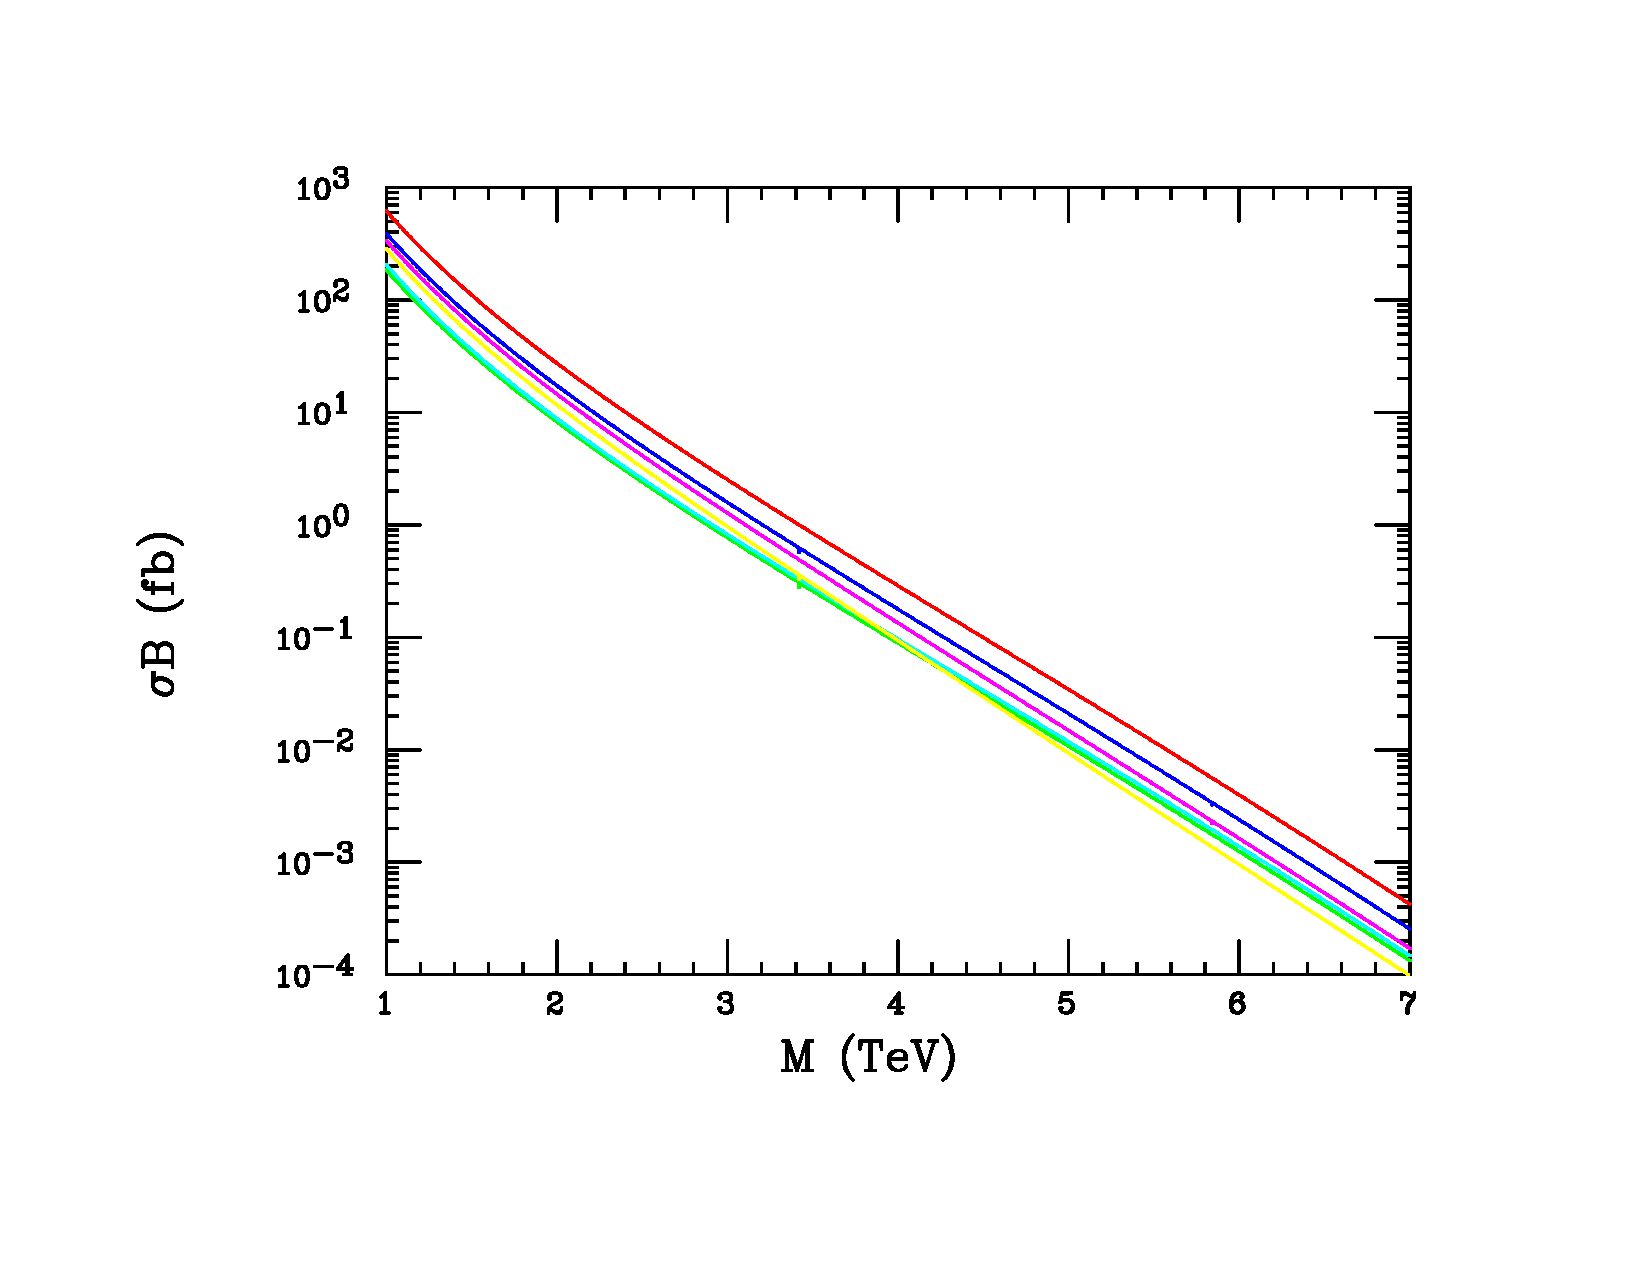
\includegraphics[trim={2cm 2cm 2cm 2cm},clip,width=0.49\columnwidth]{Fig/zp14tev-ref.pdf}
    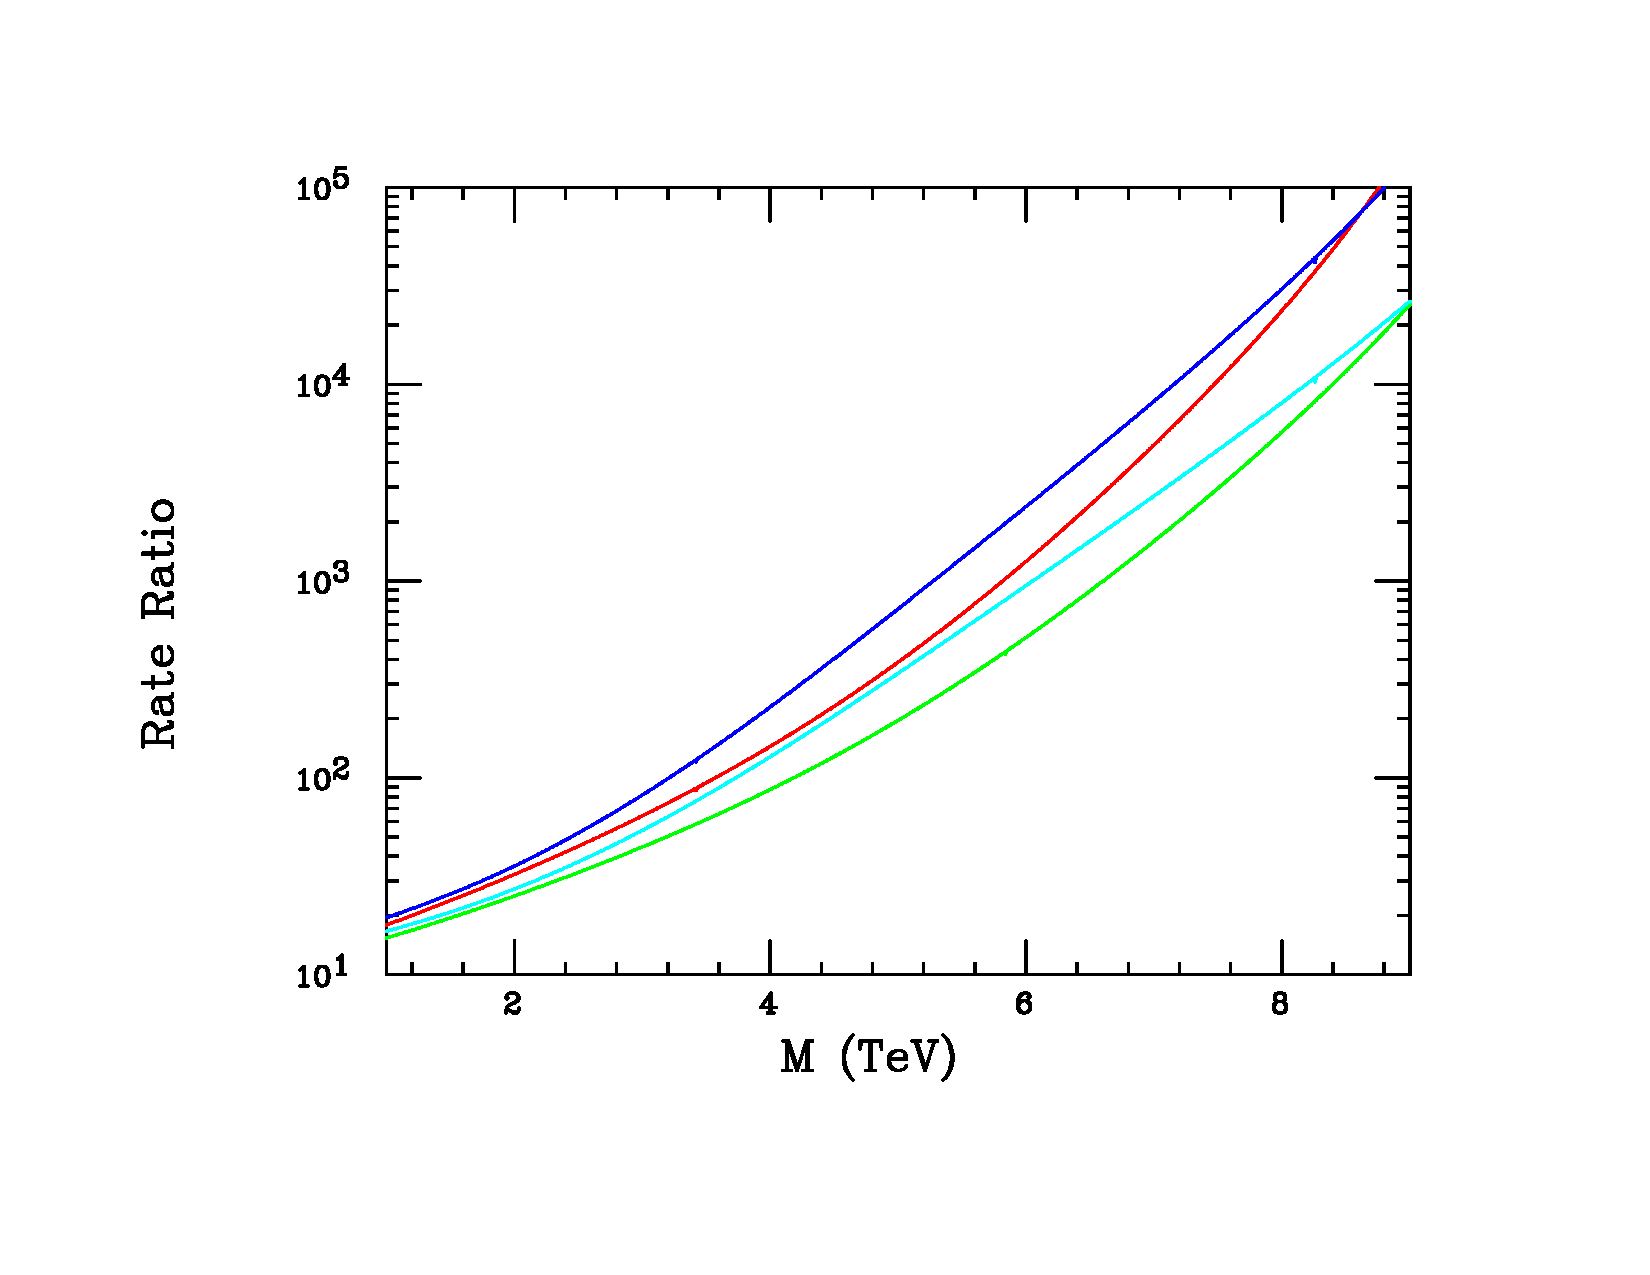
\includegraphics[trim={2cm 2cm 2cm 2cm},clip,width=0.49\columnwidth]{Fig/scaled-ratio.pdf}
\caption{(Top) $\sigma B_l$ in the NWA for the $Z'$ production at the $\sqrt s=14$ TeV LHC as functions of the $Z'$ mass: SSM(red), LRM (blue), $\psi$(green), $\chi$(magenta), 
$\eta$(cyan), I(yellow).  (Bottom) Ratio of the number of events  for $\sqrt s=27$ TeV, L=15 ab$^{-1}$ to that at 13[14] TeV, L=3 ab$^{-1}$ for 
$\bar u u$ (red) and $\bar d d$ (blue)  [green, cyan] initial state partons with fixed invariant mass $M$.}
\label{toy}
\end{figure}



%
\begin{table}
\centering
\begin{tabular}{|l|c|c|c|} \hline\hline
  Model &   95$\%$ CL     &  $3\sigma$     &   $5\sigma$   \\
\hline
SSM    &     6.62     &  6.09        &  5.62     \\
LRM    &   6.39     & 5.85        & 5.39  \\
$\psi$    &  6.10   & 5.55   & 5.07  \\
$\chi$   &  6.22    & 5.68    & 5.26   \\
$\eta$   &  6.15     &  5.59  &  5.16   \\
~I        & 5.98   &  5.45   &  5.05  \\
\hline\hline
\end{tabular}
\caption{ $\sqrt s=14$ TeV results for $M_{Z'}$ in TeV as discussed in the text. }
\label{spec}
\end{table}
%


\subsection{Discrimination from direct calculations}
Question: Can we use just this dilepton channel to distinguish between these six $Z'$ models? 
\newline
\\
We make use of 3 observables, all in NWA: $\sigma B_l$, the forward-backward asymmetry, $A_{FB}$ and the rapidity ratio, $r_y$. These last two are defined 
and discussed at some extent in both \cite{Rizzo:2014xma} and \cite{Han:2013mra}.  Given the ATLAS and CMS analyses as presented in \cite{Han:2016qpd} 
and \cite{CMS:2017zzj} we employ the entire range of rapidity $|y|\leq 2.5$ in defining these quantities. Based on these same works and \cite{Han:2013mra}, 
In addition to usual statistical errors, we will assume a $2\%$ systematic error on the two ratios as most uncertainties (lumi and PDF) will cancel between numerators 
and denominators. For $\sigma B_l$, we assign a $5\%$ systematic error in addition to this $2\%$; all errors are then added in quadrature. I am aware that these may 
be aggressive numbers but the plots will tell all. 


\begin{figure}[htbp]
  \centering
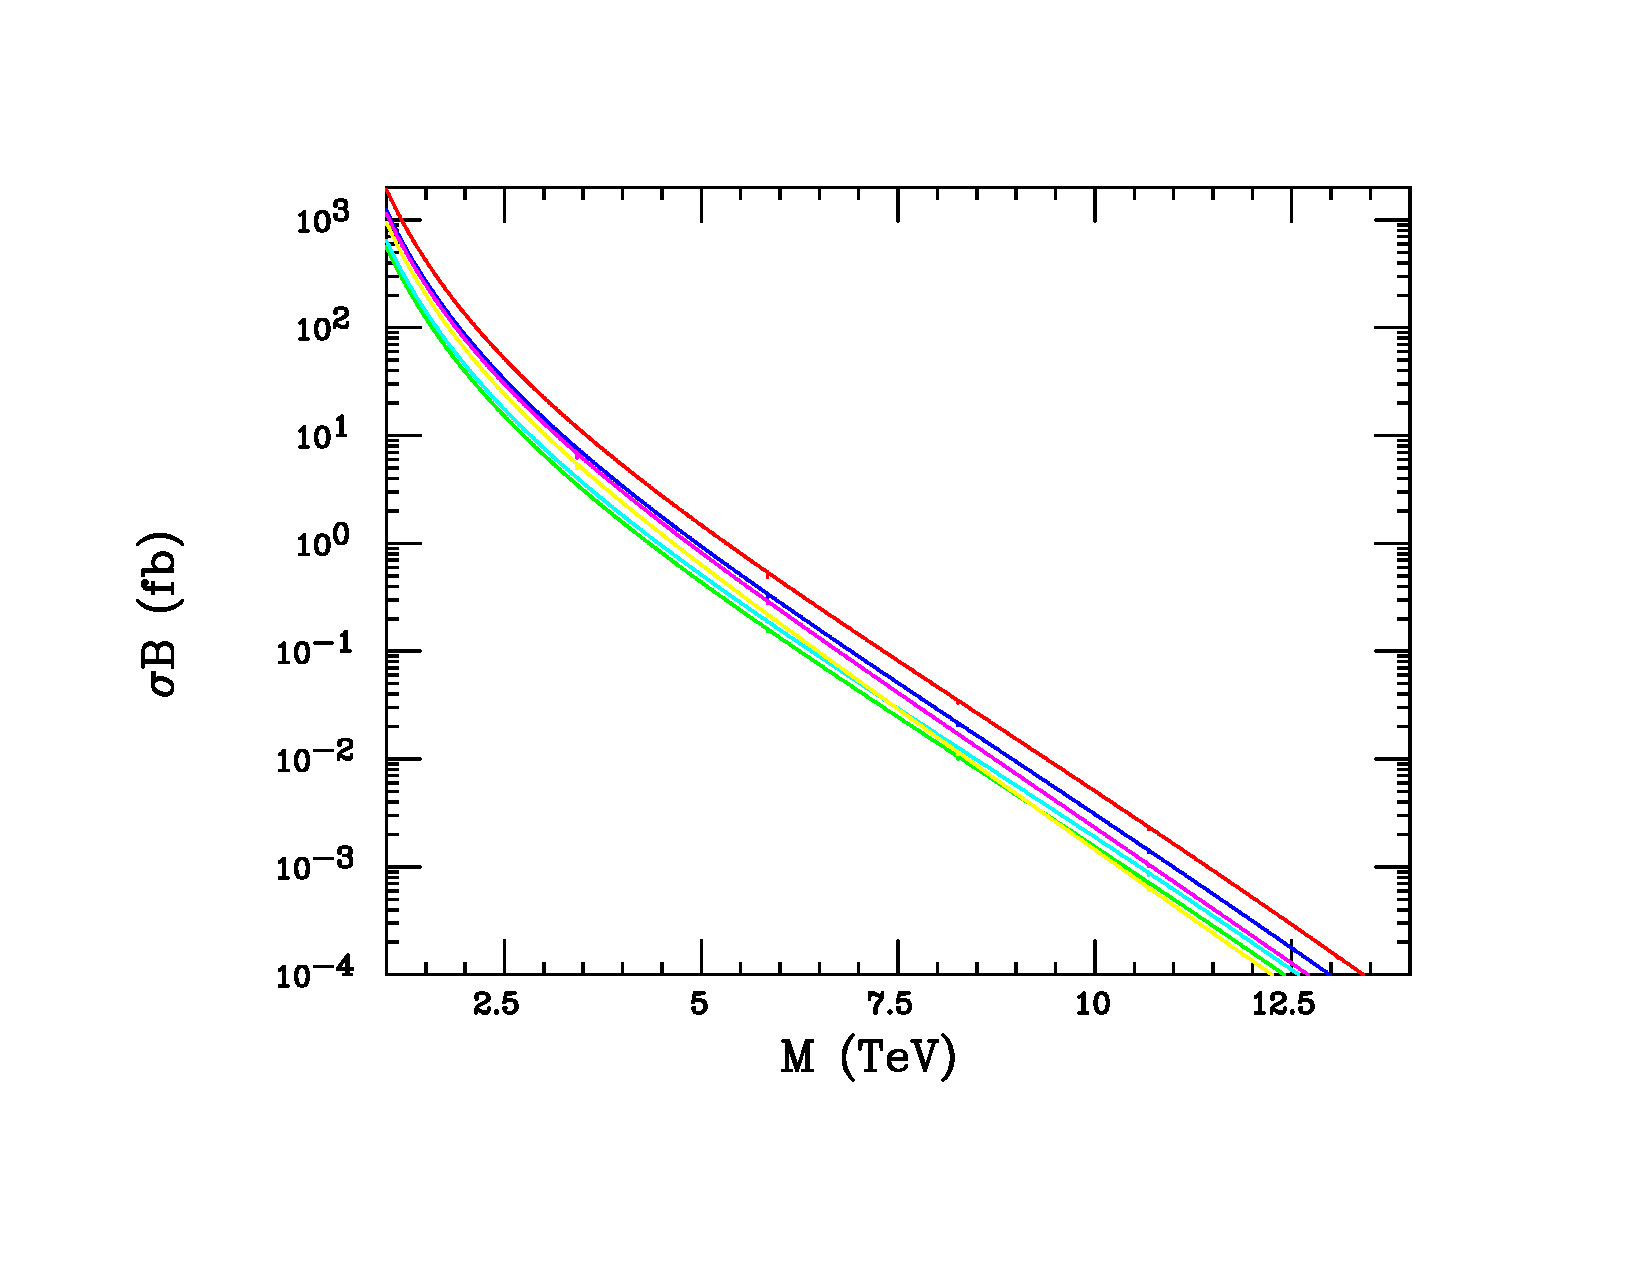
\includegraphics[trim={2cm 2cm 2cm 2cm},clip,width=0.49\columnwidth]{Fig/zp27tev-ref.pdf}
\caption{ Same as the top panel in the previous Figure but now for the HE-LHC.}
\label{toy2}
\end{figure}



Fig.~\ref{toy3} shows the correlated predictions for these 3 observables for these six models given the above assumptions and employing {\it only} a single dilepton 
channel. Here we see that apart from a possible near degeneracy in models $\psi,\eta$, a reasonable $Z'$ model separation is indeed achieved. It is clear that this 
remains possible even with somewhat larger values for the systematic errors. I note again that the use of $\sigma B_l$ relies on the absence of new non-SM decay 
modes.



\begin{figure}[htbp]
  \centering
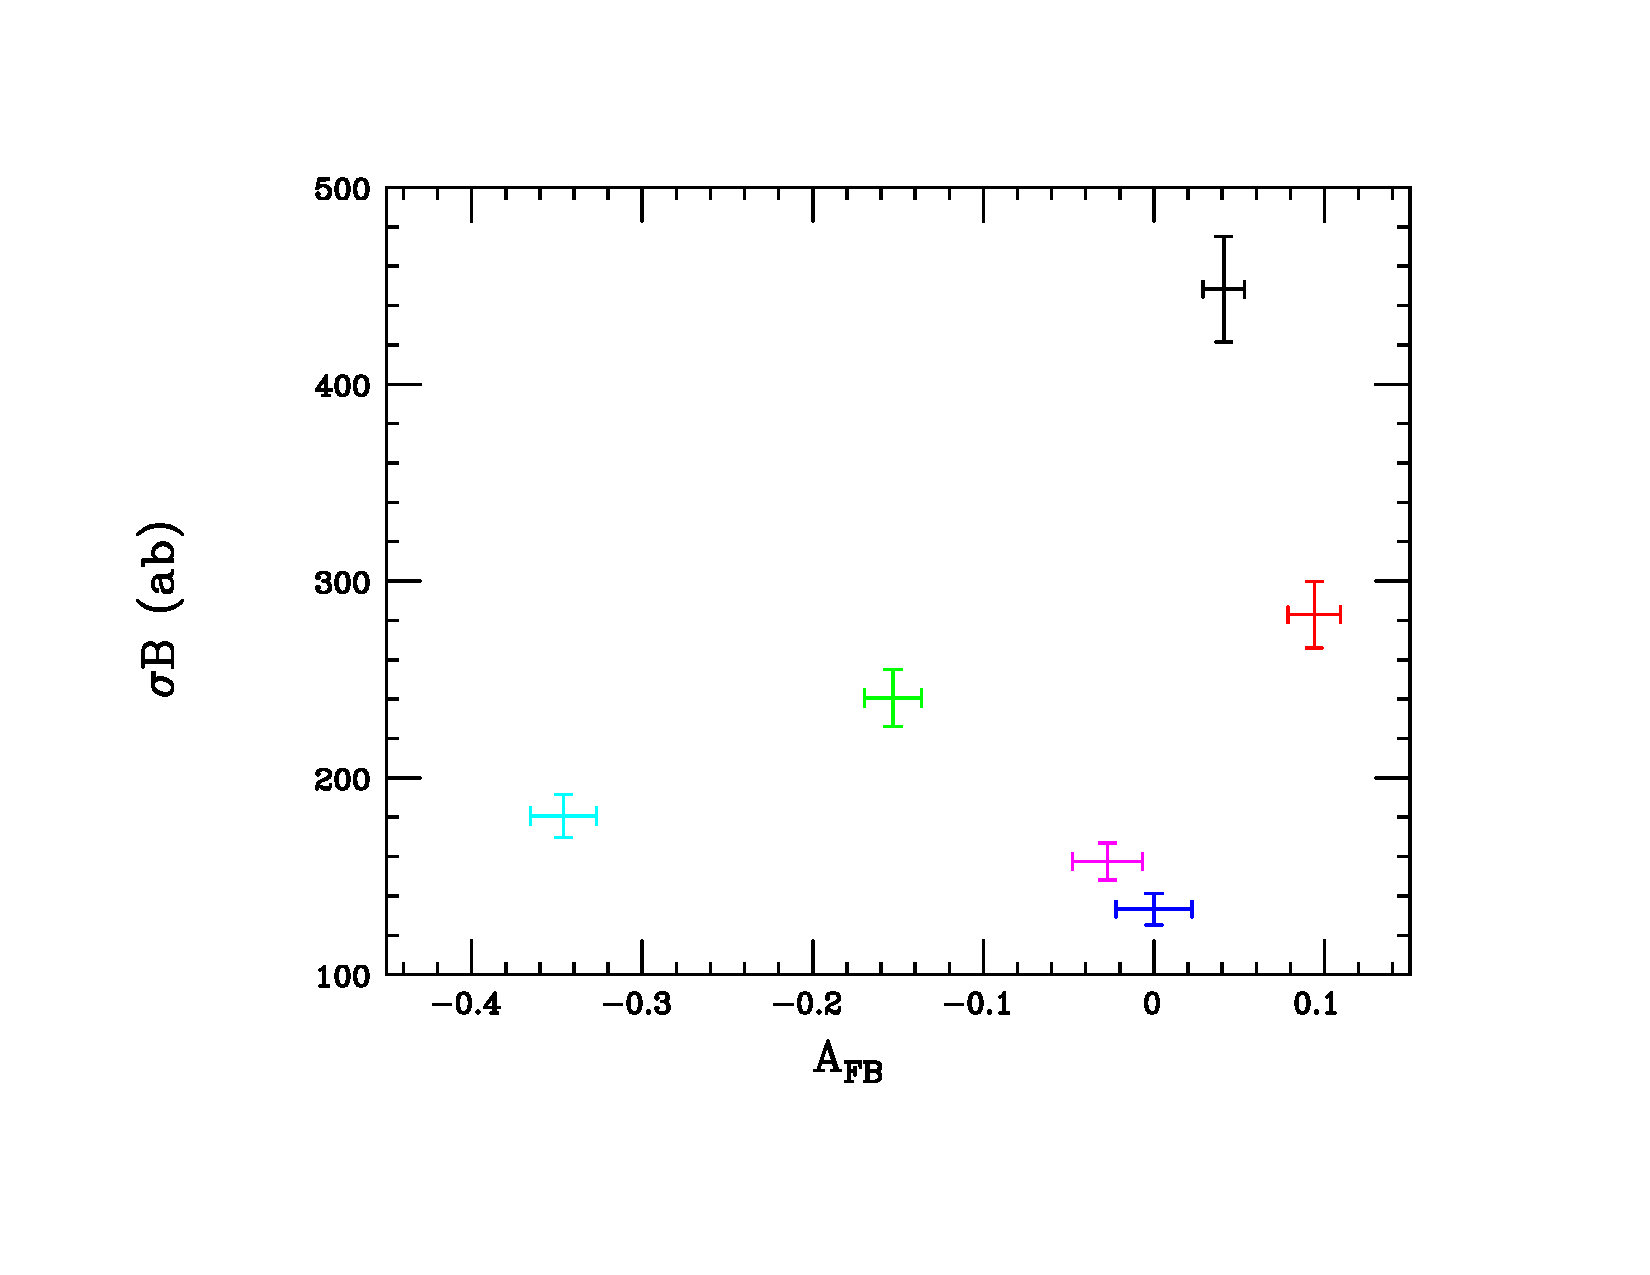
\includegraphics[trim={2cm 2cm 2cm 2cm},clip,width=0.49\columnwidth]{Fig/compare2-n.pdf}
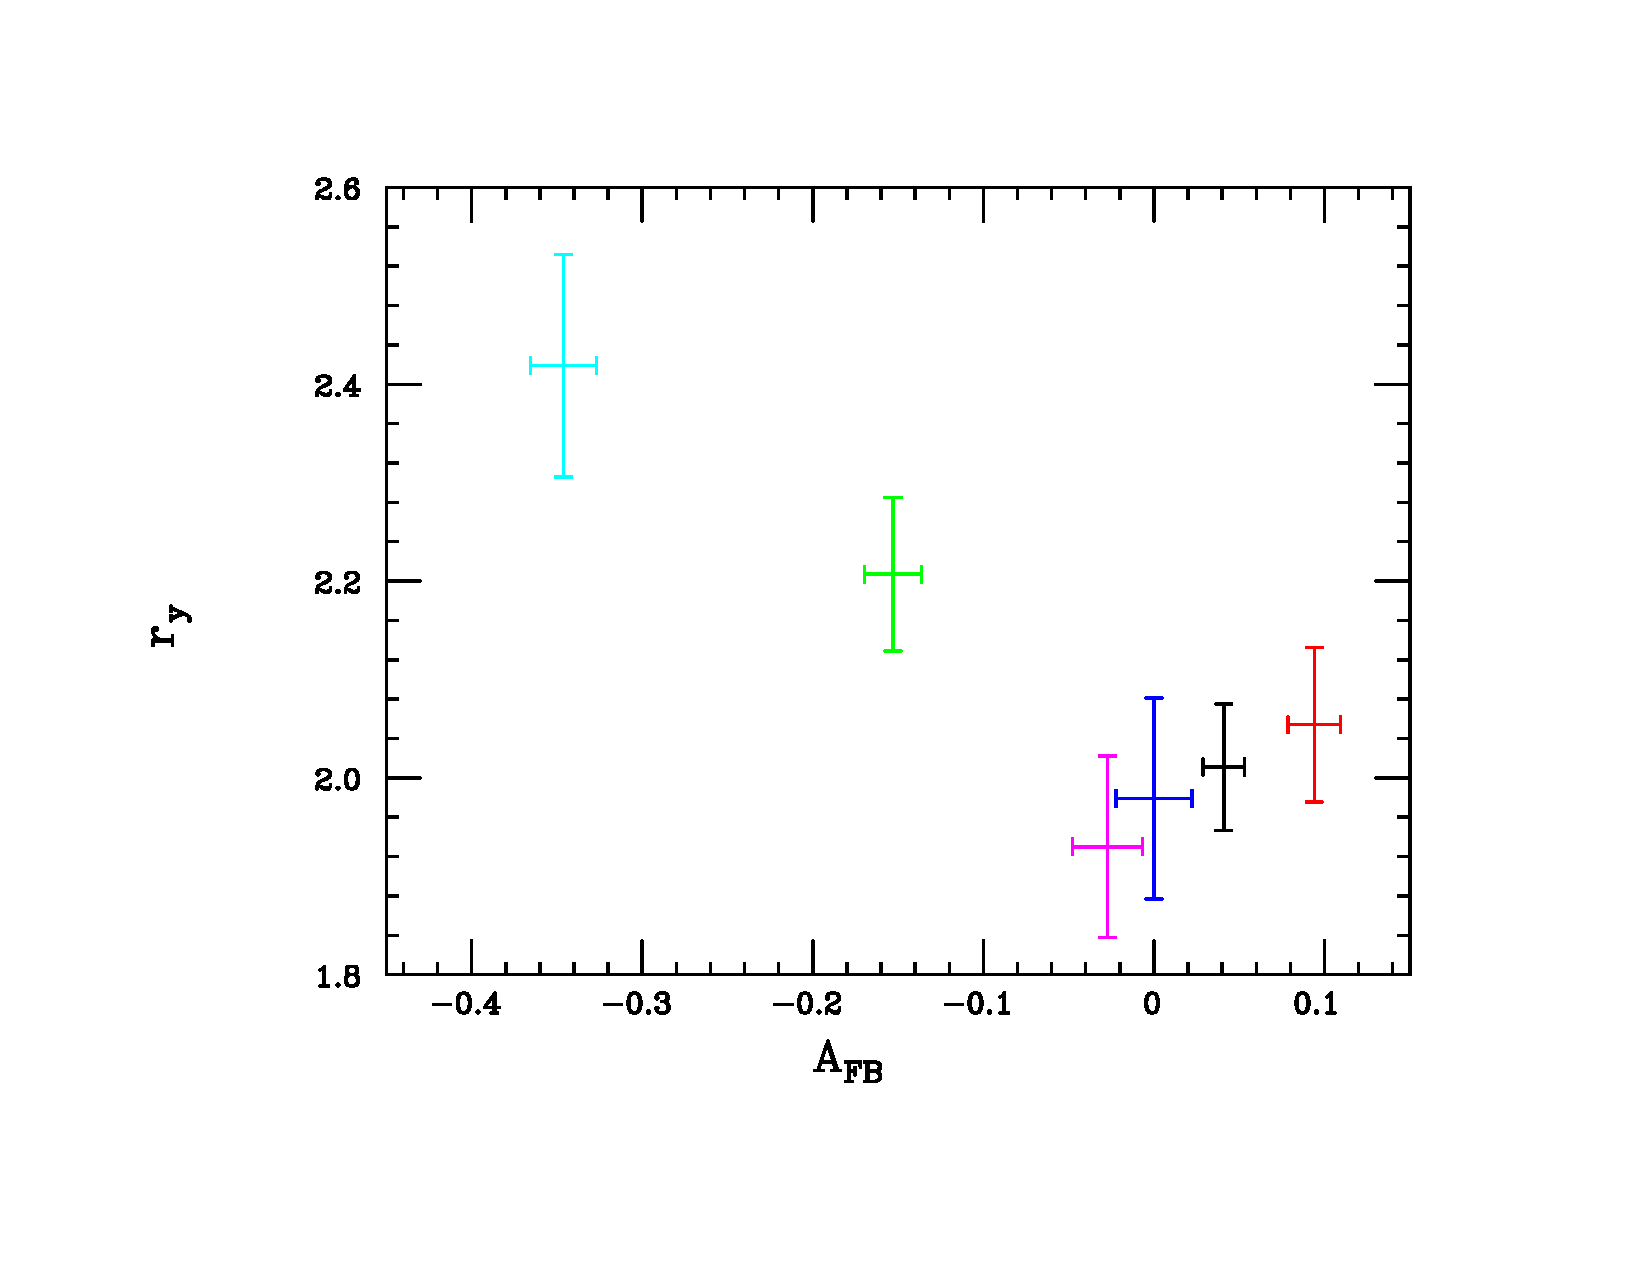
\includegraphics[trim={2cm 2cm 2cm 2cm},clip,width=0.49\columnwidth]{Fig/compare3-n.pdf}
\caption{(Top) $\sigma B_l$ vs $A_{FB}$ and (Bottom) $r_y$ vs $A_{FB}$ at the HE-LHC assuming $M_Z'=6$ TeV as discussed in the text. 
SSM(black), LRM(red), $\psi$ (blue), $\chi$ (green), $\eta$ (magenta) and I (cyan). $1\sigma$ errors only are shown. }
\label{toy3}
\end{figure}




\subsection{Discrimination from detector level analysis}
The analyses presented in this section are all performed within the FCC software framework, FCCSW~\cite{fccsw_web}.
The detector parametrisation considered in this study is from HE-LHC official parametrisation for the yellow report~\cite{hlhelhc_web}.
The Monte Carlo are first presented in Section~\ref{subsection:MC} Leptonic decays are presented in~\ref{subsection:lepana}, and hadronic analyses in~\ref{subsection:hadana}.


\subsubsection{Monte Carlo Samples}
\label{subsection:MC}
Monte Carlo~(MC) simulated event samples were used to simulate the response of the FCC detector to signal and backgrounds. The muon momentum resolution 
is assumed to be $\sigma(p)/p \approx 20\%$ at $\pt= 20 $TeV. Signals are generated with {\scshape Pythia}~8.230~\cite{Sjostrand:2014zea} using the leading 
order cross-section from the generator. All lepton flavour decays of the $Z'$ are generated assuming universality of the couplings.
The Drell-Yan background has been generated using {\scshape MG5\_}a{\scshape MC@NLO}~2.5.2~\cite{Alwall:2014hca} at leading order only. 
A k-factor of 2 is applied to all the background processes. The PDF used is NNPDF3.1 QCD LO $\alpha_{s}(M_Z) = 0.118$.



\subsubsection{Leptonic analysis}
\label{subsection:lepana}
\subsubsubsection{Event selection and discovery potential}

Events are required to contain at least two same flavour leptons of opposite charge with $\pt > 500$~GeV, $|\eta|<$4.5. 
When mentioned a smaller acceptance of $|\eta|<$2.5 is considered to test the impact on the reduction of the statistics. 
An additional cut on the di-lepton invariant mass $m_{ll}>1$~TeV is applied to remove the low mass Drell-Yan. 
Figure~\ref{figure:lepana:mass} shows the invariant mass for a 6~TeV signal for the $ee$ (left) and $\mu\mu$ channels (right). 
The mass resolution is better for the ee channel, as expected from the higher performance of the electro-magnetic calorimeter at high energy.

\label{sec:lepana}
\begin{figure}[h]
  \centering
    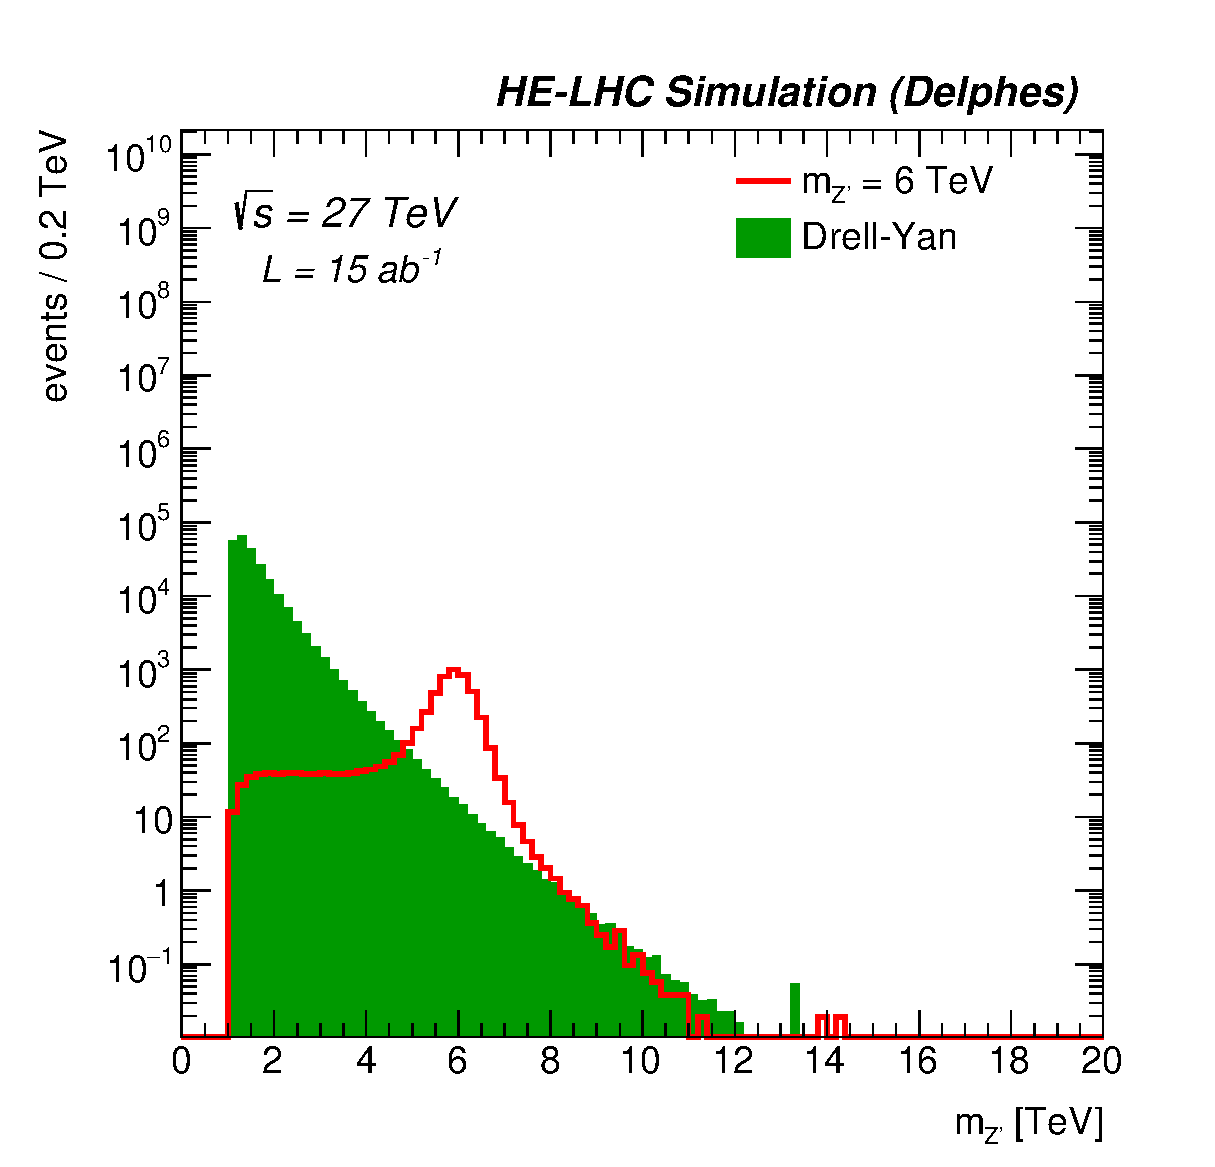
\includegraphics[width=0.45\columnwidth]{Fig/Zpmumu_mzp_sel0_nostack_log.eps}
    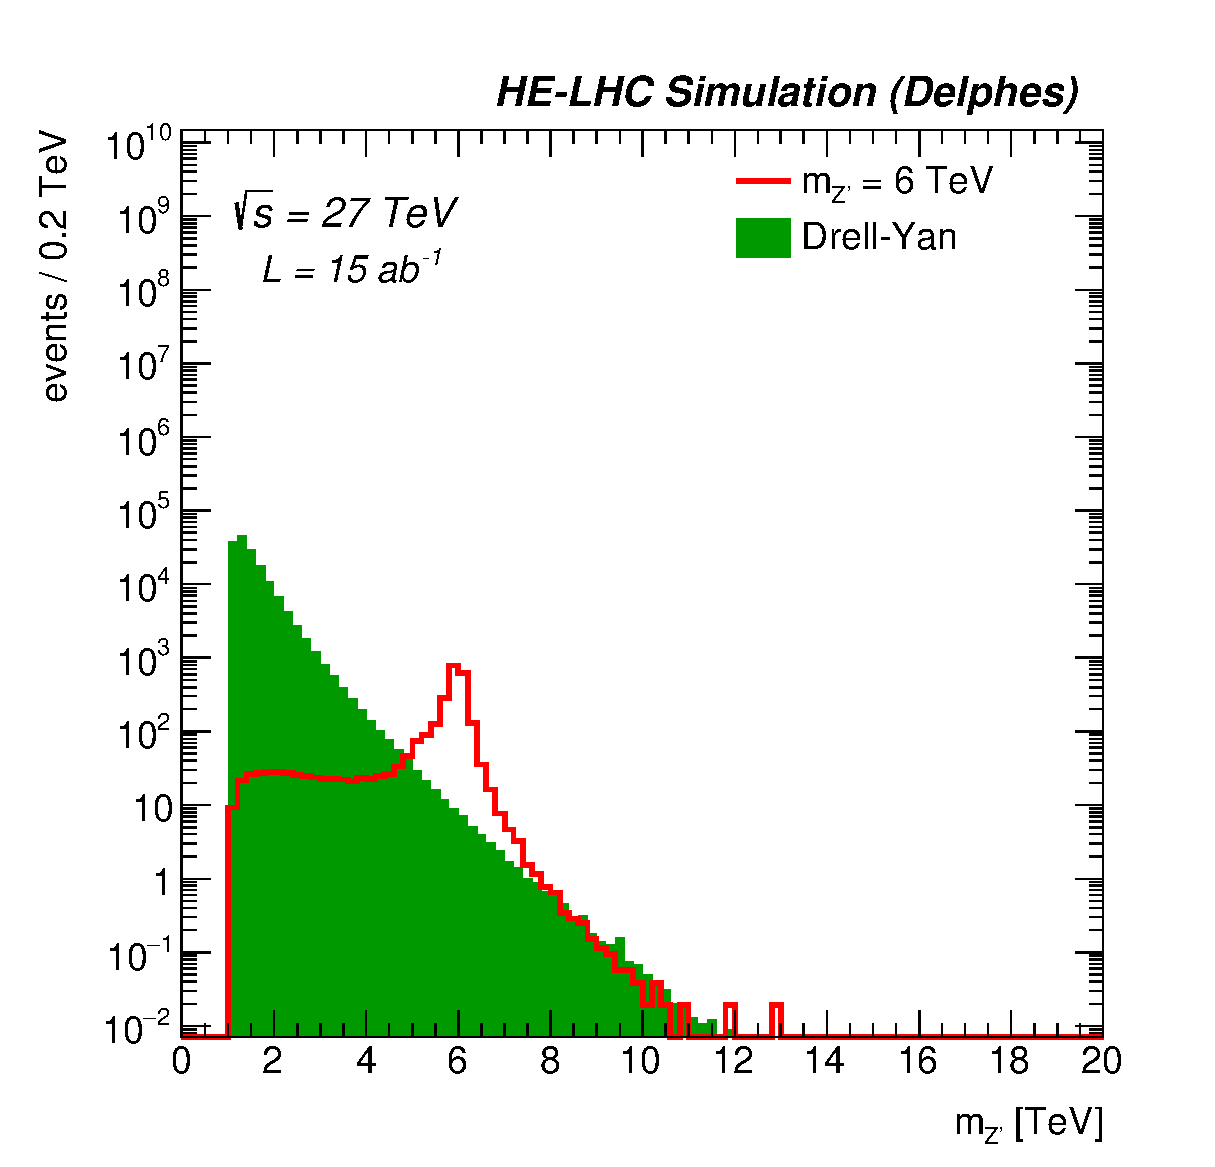
\includegraphics[width=0.45\columnwidth]{Fig/Zpee_mzp_sel0_nostack_log.eps}
   \caption{Invariant mass for a 6~TeV signal after full event selection for ee channel (left) and $\mu\mu$ channel (right).}
  \label{figure:lepana:mass}
\end{figure}

Limits and discovery potential for di-lepton resonances are shown in Figure~\ref{figure:lepana:limdisc}. With the full 15~ab$^{-1}$ 
integrated luminosity, it is expected to exclude heavy $Z'$ resonances from 10 to 12.5~TeV depending on the model and discover 
a $Z'_{SSM}$ up to 12~TeV.

\begin{figure}[!htb]
  \centering
  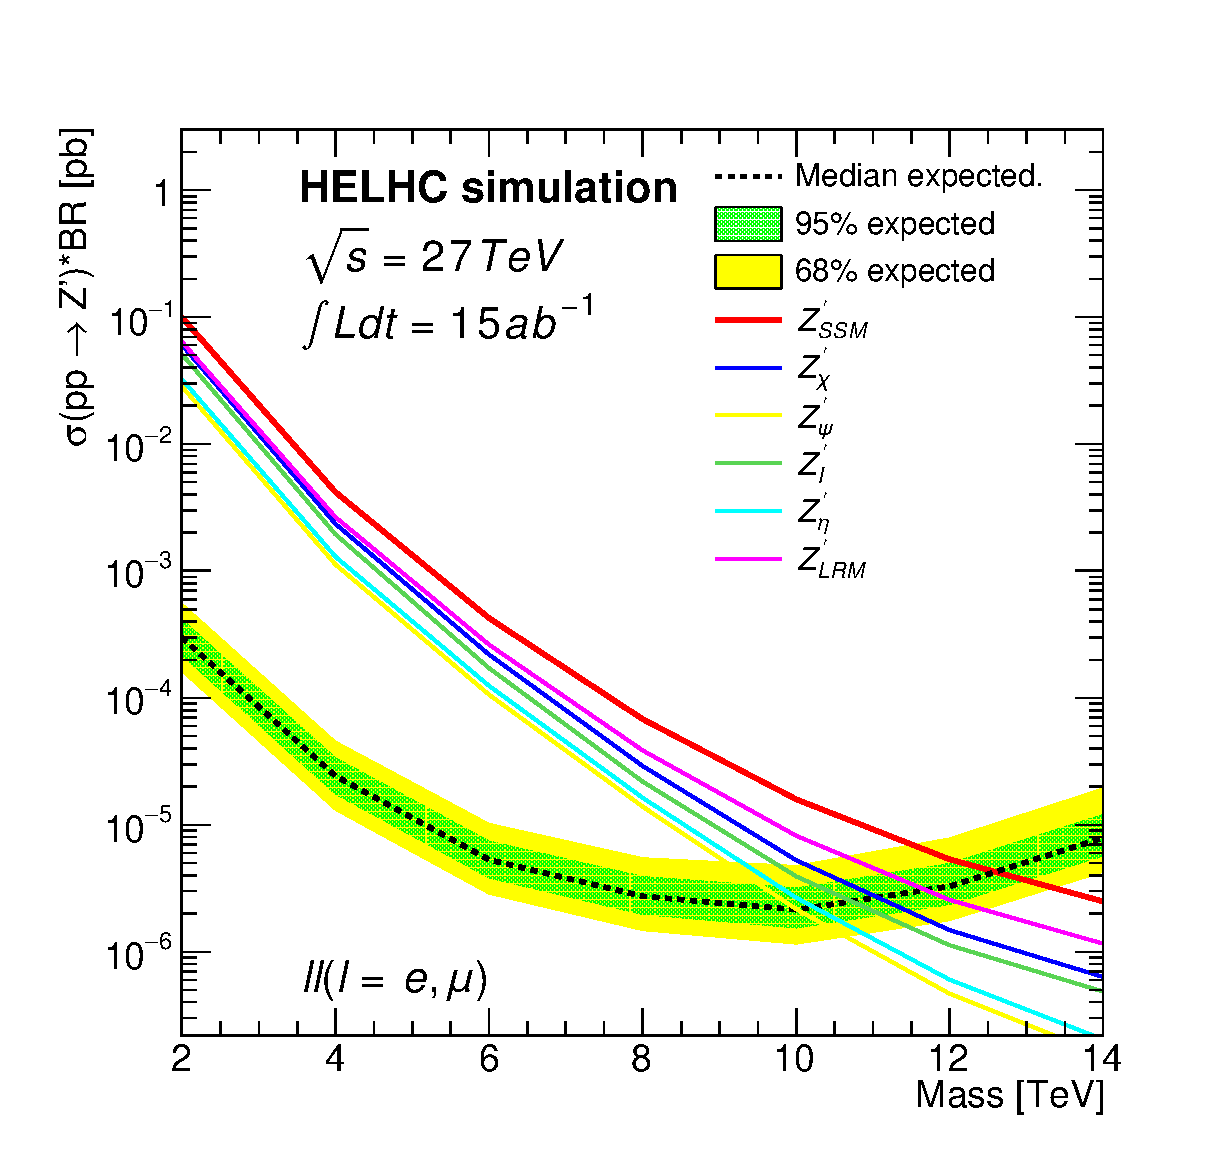
\includegraphics[width=0.45\columnwidth]{Fig/lim_Zprime_ll_helhc_v01_allxs.eps}
  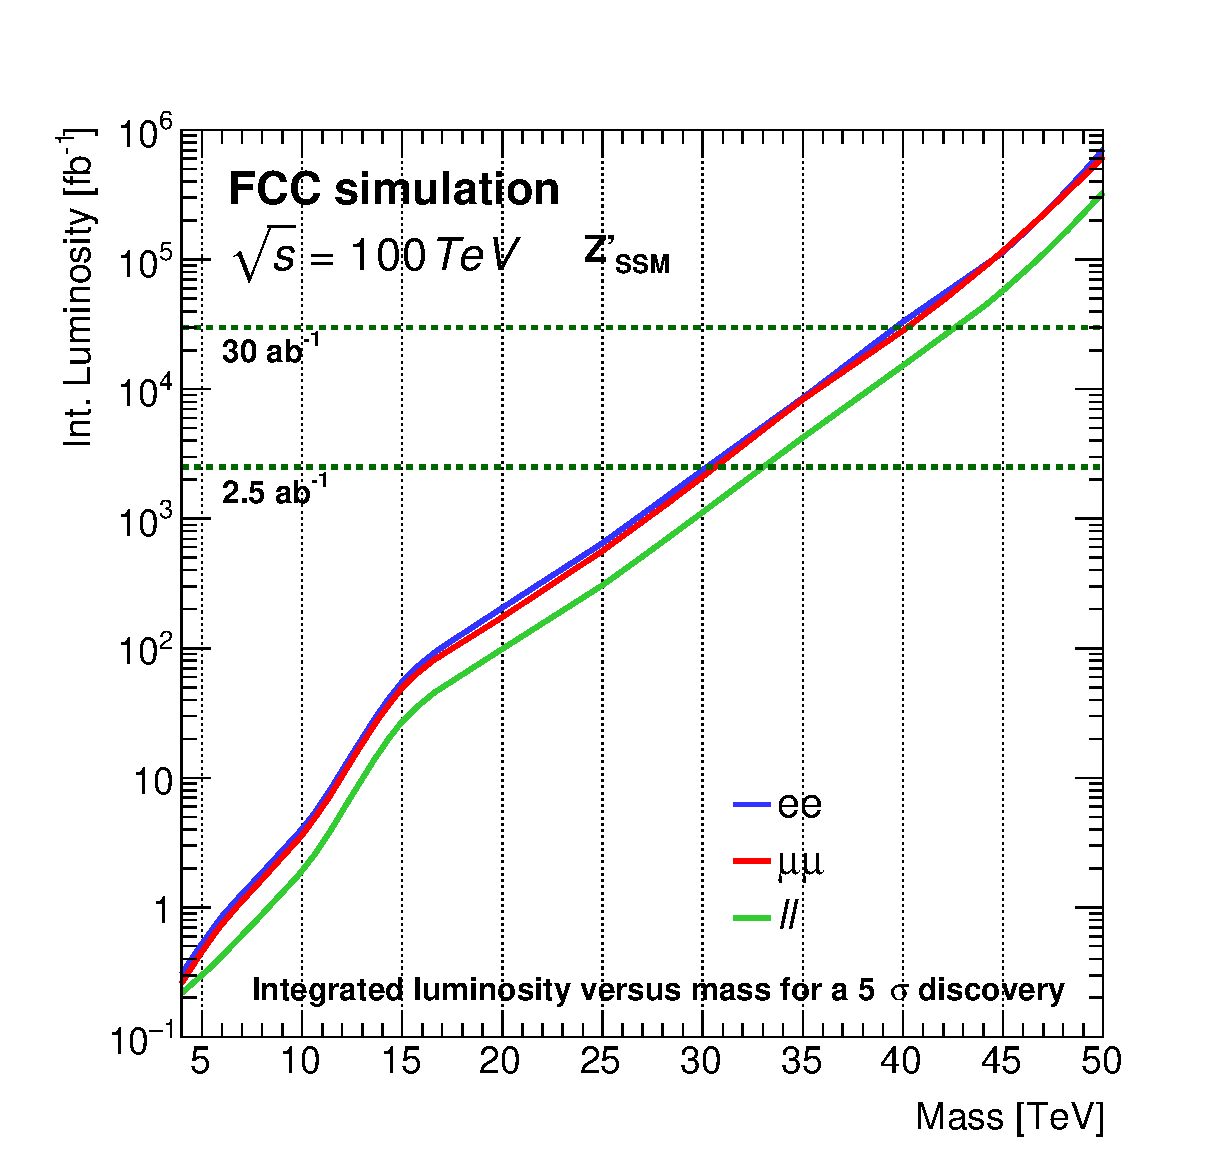
\includegraphics[width=0.45\columnwidth]{Fig/DiscoveryPotential_ll_comb_rootStyle.eps}
  \caption{Limit versus mass for the di-lepton channel (left) and luminosity for a $5\sigma$ discovery (right) for the ee and $\mu\mu$ combined channels. }
  \label{figure:lepana:limdisc}
\end{figure}


\subsubsubsection{Variables definition}
\label{subsubsection:vardef}

As for the analysis from direct calculation, the observables are defined at the detector level. On Figure~\ref{figure:lepana:yzp} the 
rapidity of the $Z'$ is displayed, and as expected it is much more central for the signal than for the Drell-Yan background.
\begin{figure}[!htb]
  \centering
  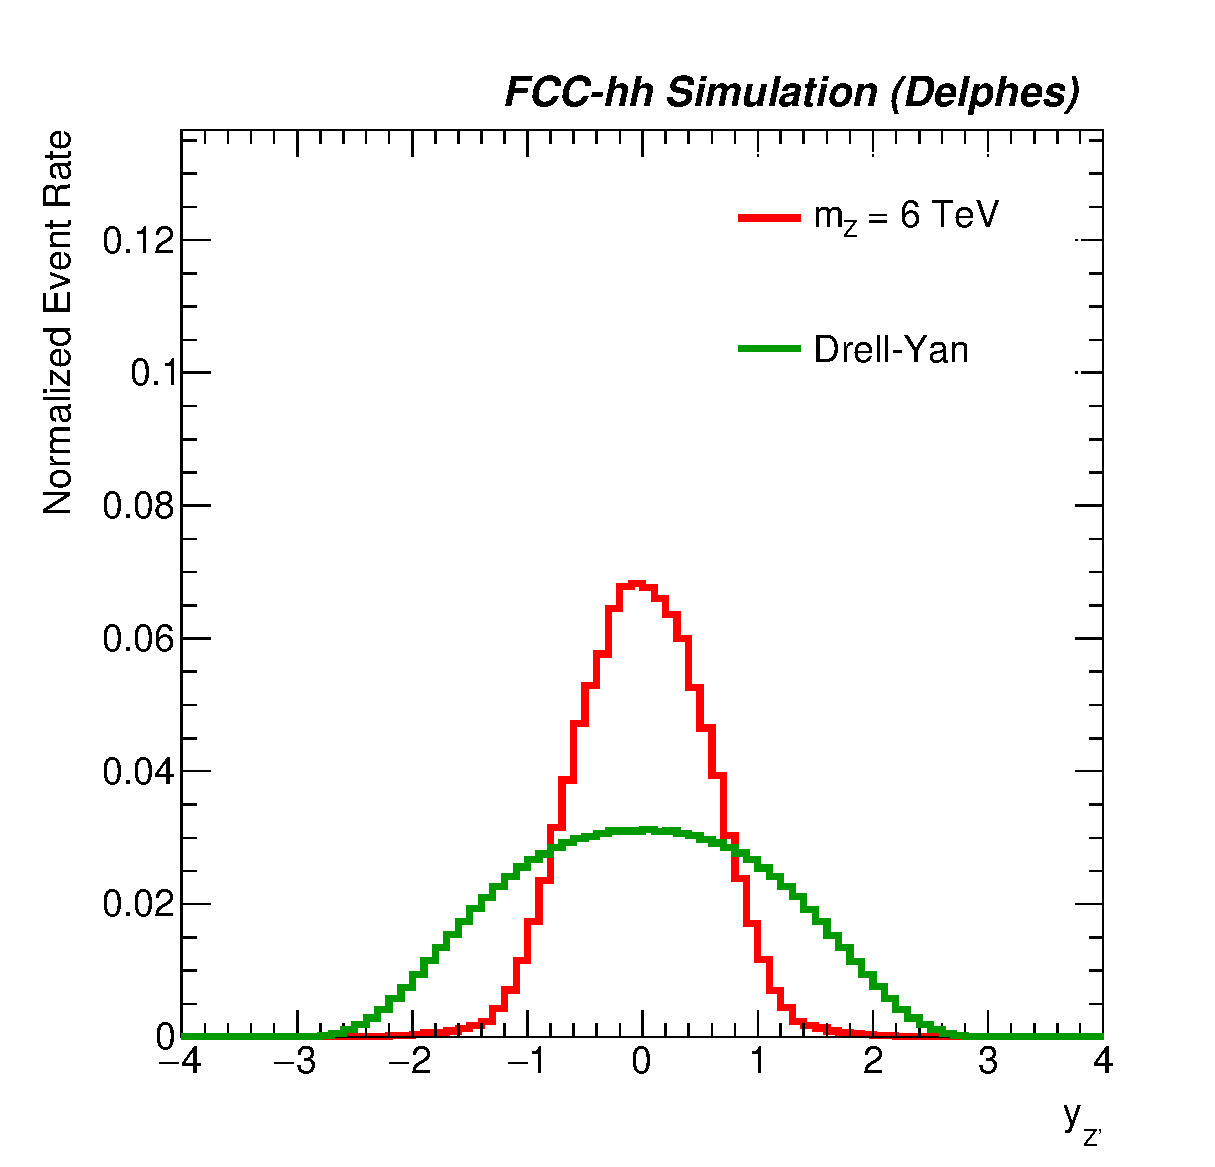
\includegraphics[width=0.45\columnwidth]{Fig/27tev/yzp_sel0_lin_norm_ee.eps}
  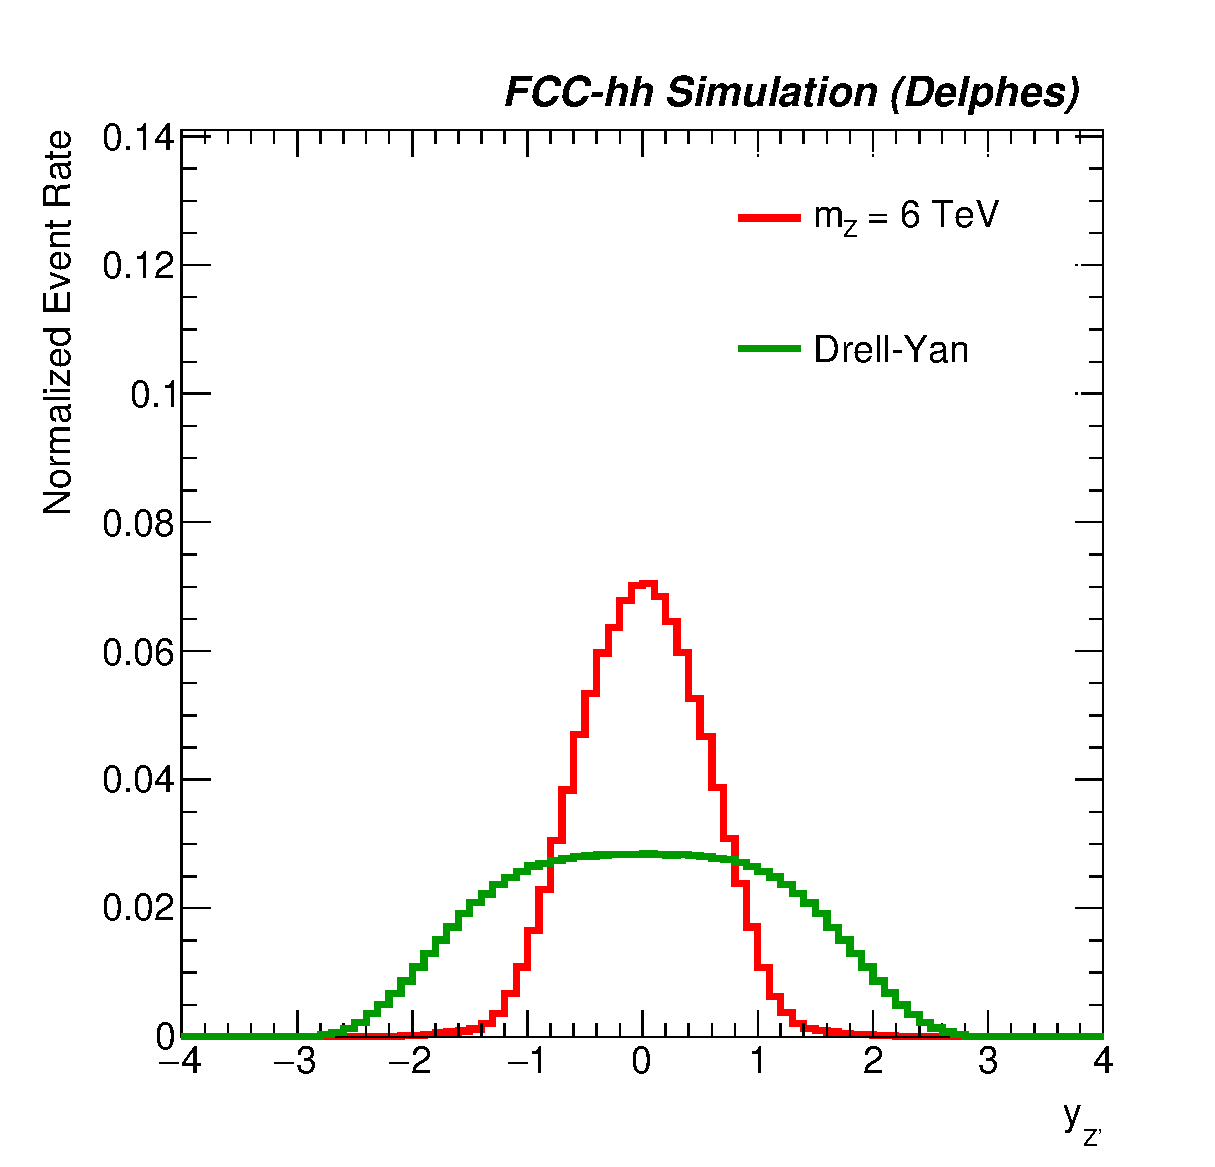
\includegraphics[width=0.45\columnwidth]{Fig/27tev/yzp_sel0_lin_norm_mumu.eps}
  \caption{$Z'$ rapidity distribution comparing a 6~TeV signal and Drell-Yan background for ee (left) and $\mu\mu$ channels (right).}
  \label{figure:lepana:yzp}
\end{figure}
At detector level the variable $r_y$ is defined as the ratio of central over forward events:
\begin{equation}
r_y = \frac{\sigma(|y_{Z'}| < y_1)}{\sigma(y_1 < |y_{Z'}| <y_2)}
\end{equation}
with $y_1=0.5$ and $y_2=2.5$ for this study.
\newline
The variable $A_{FB}$ can be seen as a measure of the charge asymmetry
\begin{equation}
A_{FB} = A_C =  \frac{\sigma(\Delta|y| > 0) - \sigma(\Delta|y| < 0)}{\sigma(\Delta|y| > 0) + \sigma(\Delta|y| < 0)}
\end{equation}
where $\Delta|y| = |y_l| - |y_{\bar{l}}|$. It has been checked that this definition is equivalent to defining 
\begin{equation}
A_{FB} =   \frac{\sigma_F - \sigma_B}{\sigma_F + \sigma_B}
\end{equation}
with $\sigma_F = \sigma (cos\theta^{*}_{cs})>0$ and $\sigma_B = \sigma (cos\theta^{*}_{cs})<0$ and defining $\theta^*$ in the Collins-Soper 
frame as
\begin{equation}
cos\theta^{*}_{cs} =  \frac{Q_z}{|Q_z|} \frac{2(P_l^+P_{\bar{l}}^- - P_l^-P_{\bar{l}}^+)}{|Q| \sqrt{Q^2+Q^2_T}}
\end{equation}
where $Q$, $Q_T$ and $Q_z$ are the four-momentum, the transverse momentum, and the longitudinal
momentum of the di-lepton pair. $P_{l}(P_{\bar{l}})$ represents the four momenta of the lepton (anti-lepton),
and $P^\pm_l = (P^0_l \pm P^3_l)$.
\newline
The last discriminating variable that is used is the fitted signal cross section $\sigma_{Z'}$. It is extracted from a profile likelihood fit.

\subsubsubsection{Optimisations}
\label{subsubsection:opti}
In Figure~\ref{figure:lepana:afb_dm} is represented $A_{FB}$ verus the acceptance window around a 6~TeV signal. 
It is shown for signal only (top-left) and is flat as expected. Once background is introduced without uncertainties (top-right), and when the window 
becomes too large the asymmetry is diluted. When adding a 10\% uncertainty on the background (bottom-left) we observe as expected larger errors and quicker dilution.
The last plot (bottom-left) shows the same variable, but considering the full interference between the signal and the Drell-Yan. One can immediately 
note the fact that the dilution goes in opposite direction as when not considering the interference. 
When considering signal only, the error bars directly represents the diminution of the statical error from adding more events. It is clear that considering a mass window cut 
larger than 500~GeV does not improve the statistical component of the signal asymmetry. When considering background without the interference, if the mass window is too large 
the discrimination potential gets worse due to dilution. In addition, if the error on the background is not controlled at a level of the order of 10\% the error on $A_{FB}$ tends to 
increase at large mass window values. When the interference between signal and Drell-Yan is considered, for very small values ($\sim$200~GeV) of the mass window 
$A_{FB}$ seems consistent with not considering the interference. 

\begin{figure}[!htb]
  \centering
   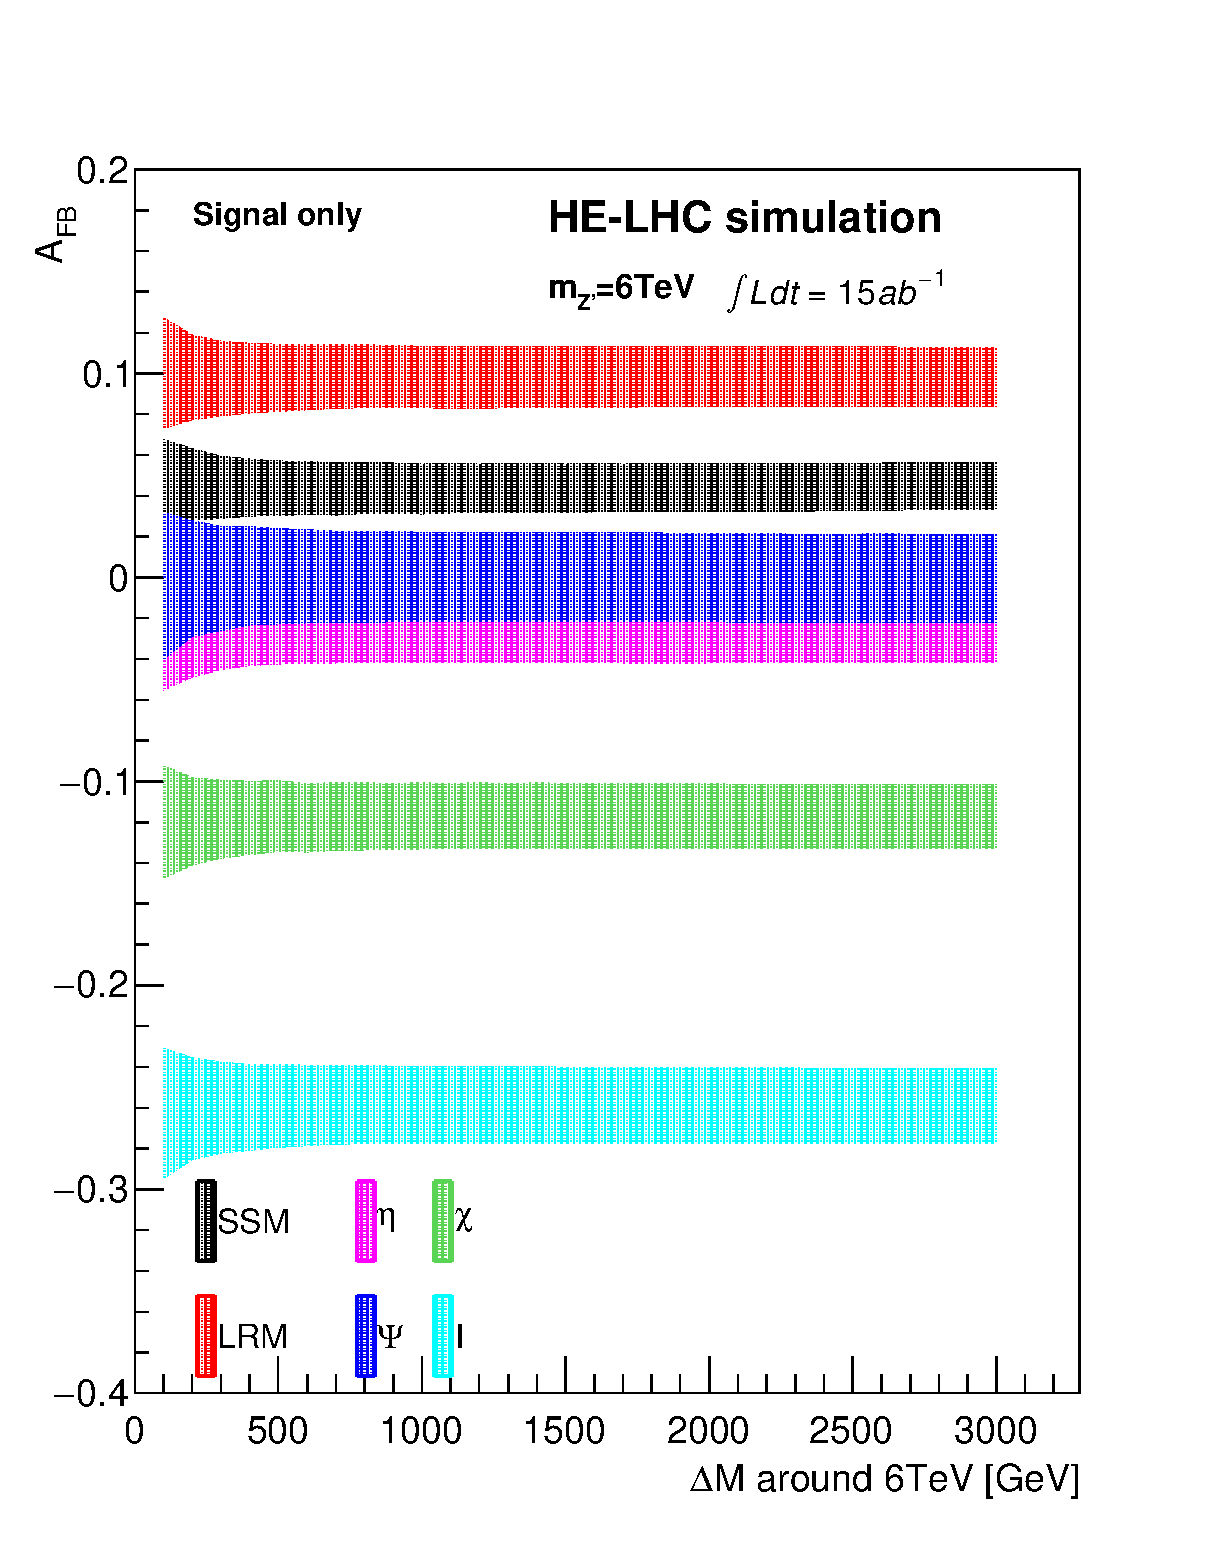
\includegraphics[width=0.45\columnwidth]{Fig/27tev/afb_vs_dm_nobg.eps}
   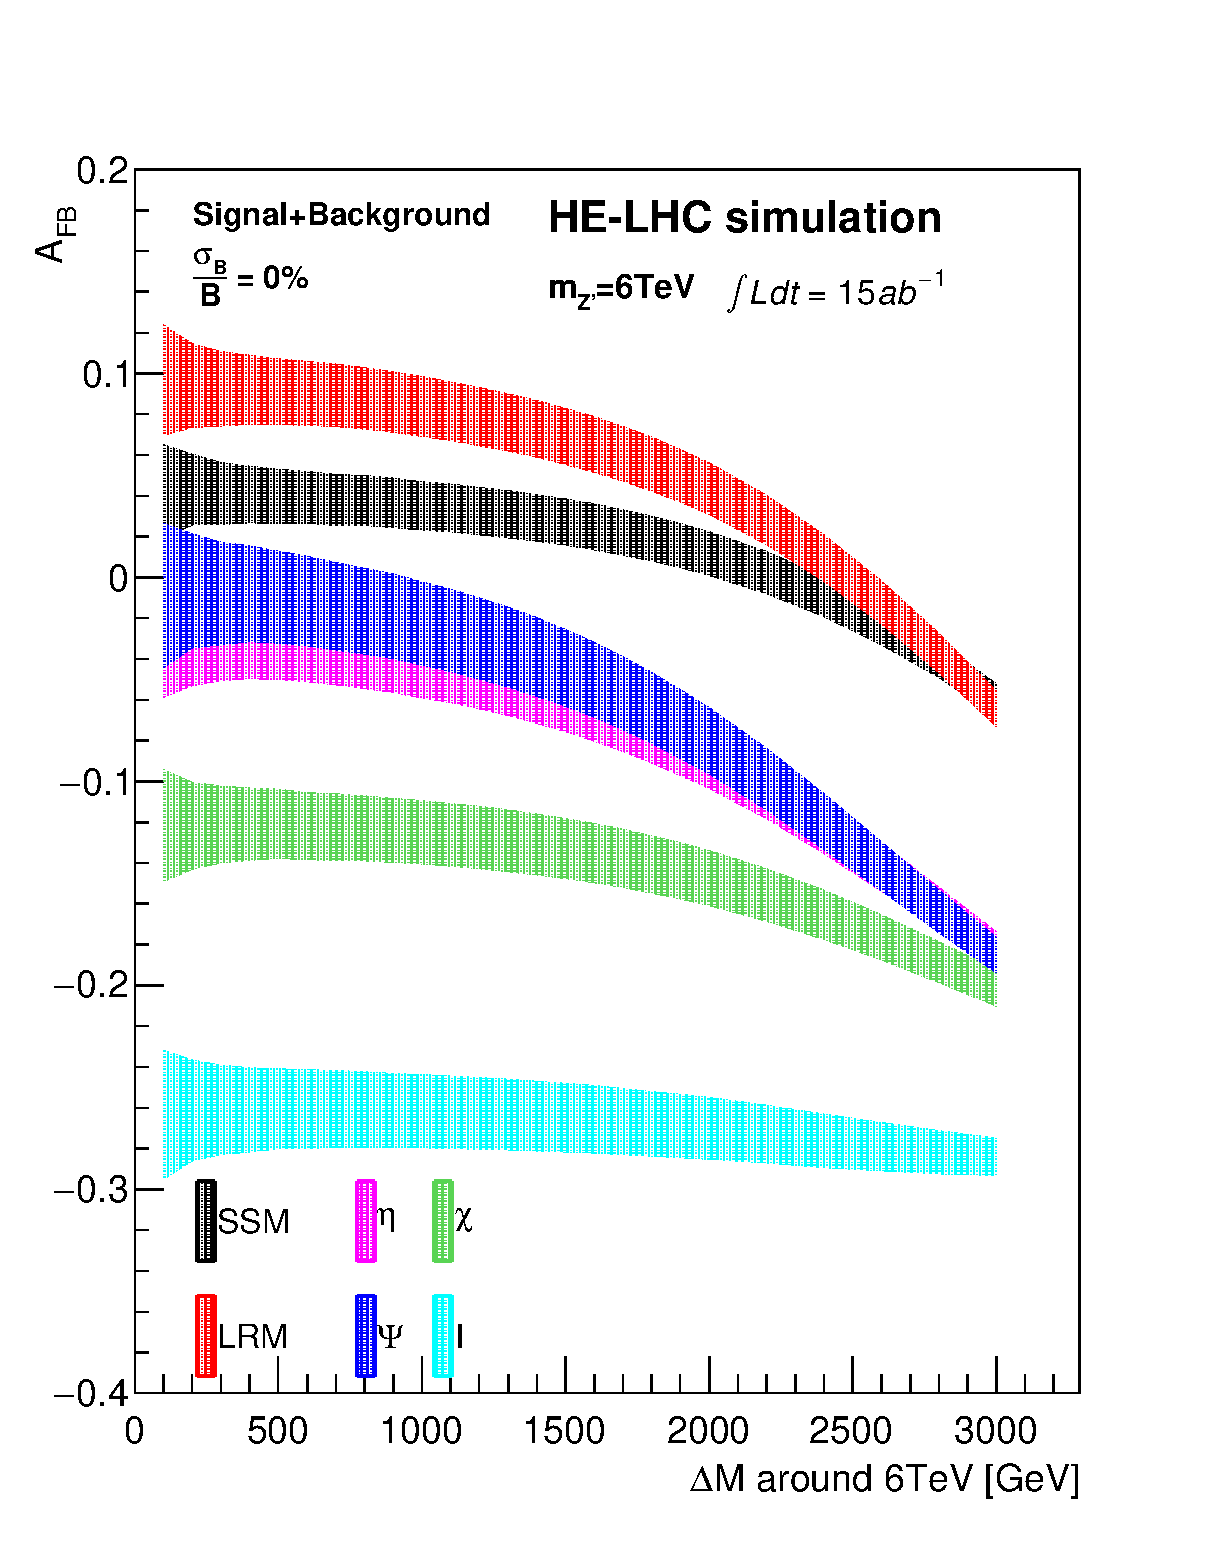
\includegraphics[width=0.45\columnwidth]{Fig/27tev/afb_vs_dm_0p.eps}
   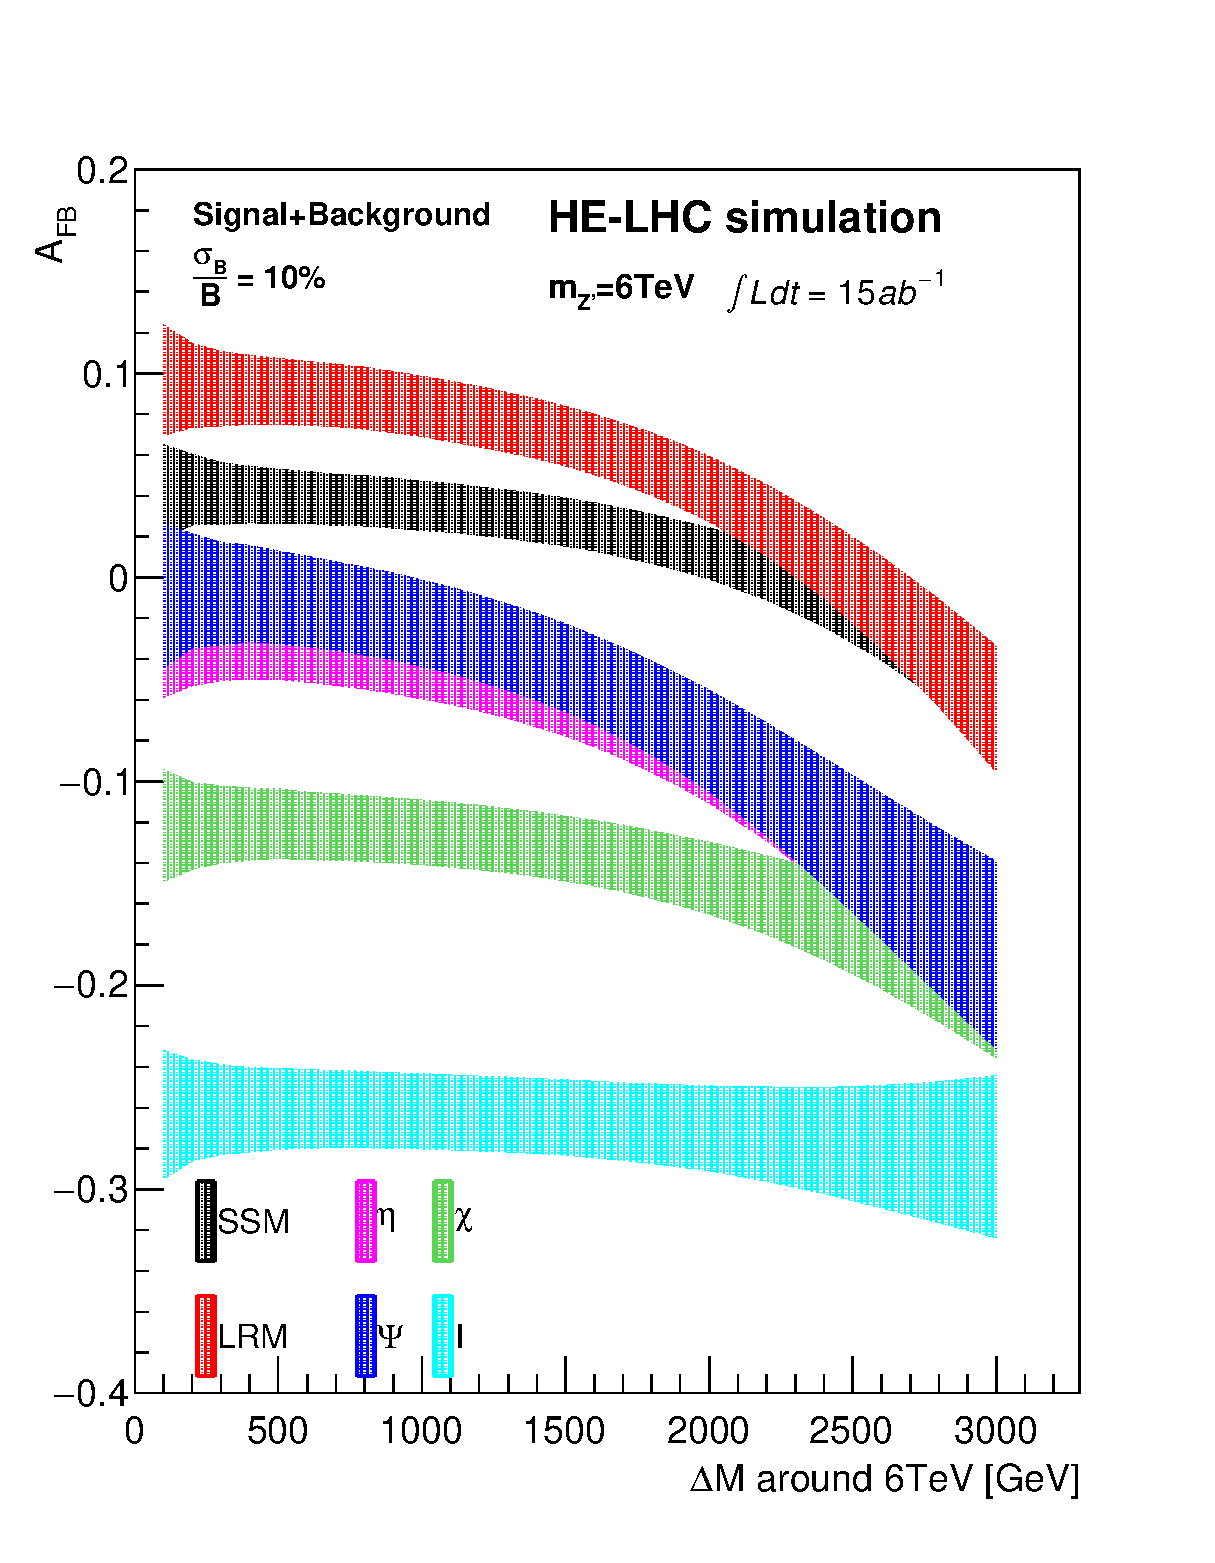
\includegraphics[width=0.45\columnwidth]{Fig/27tev/afb_vs_dm_10p.eps}
   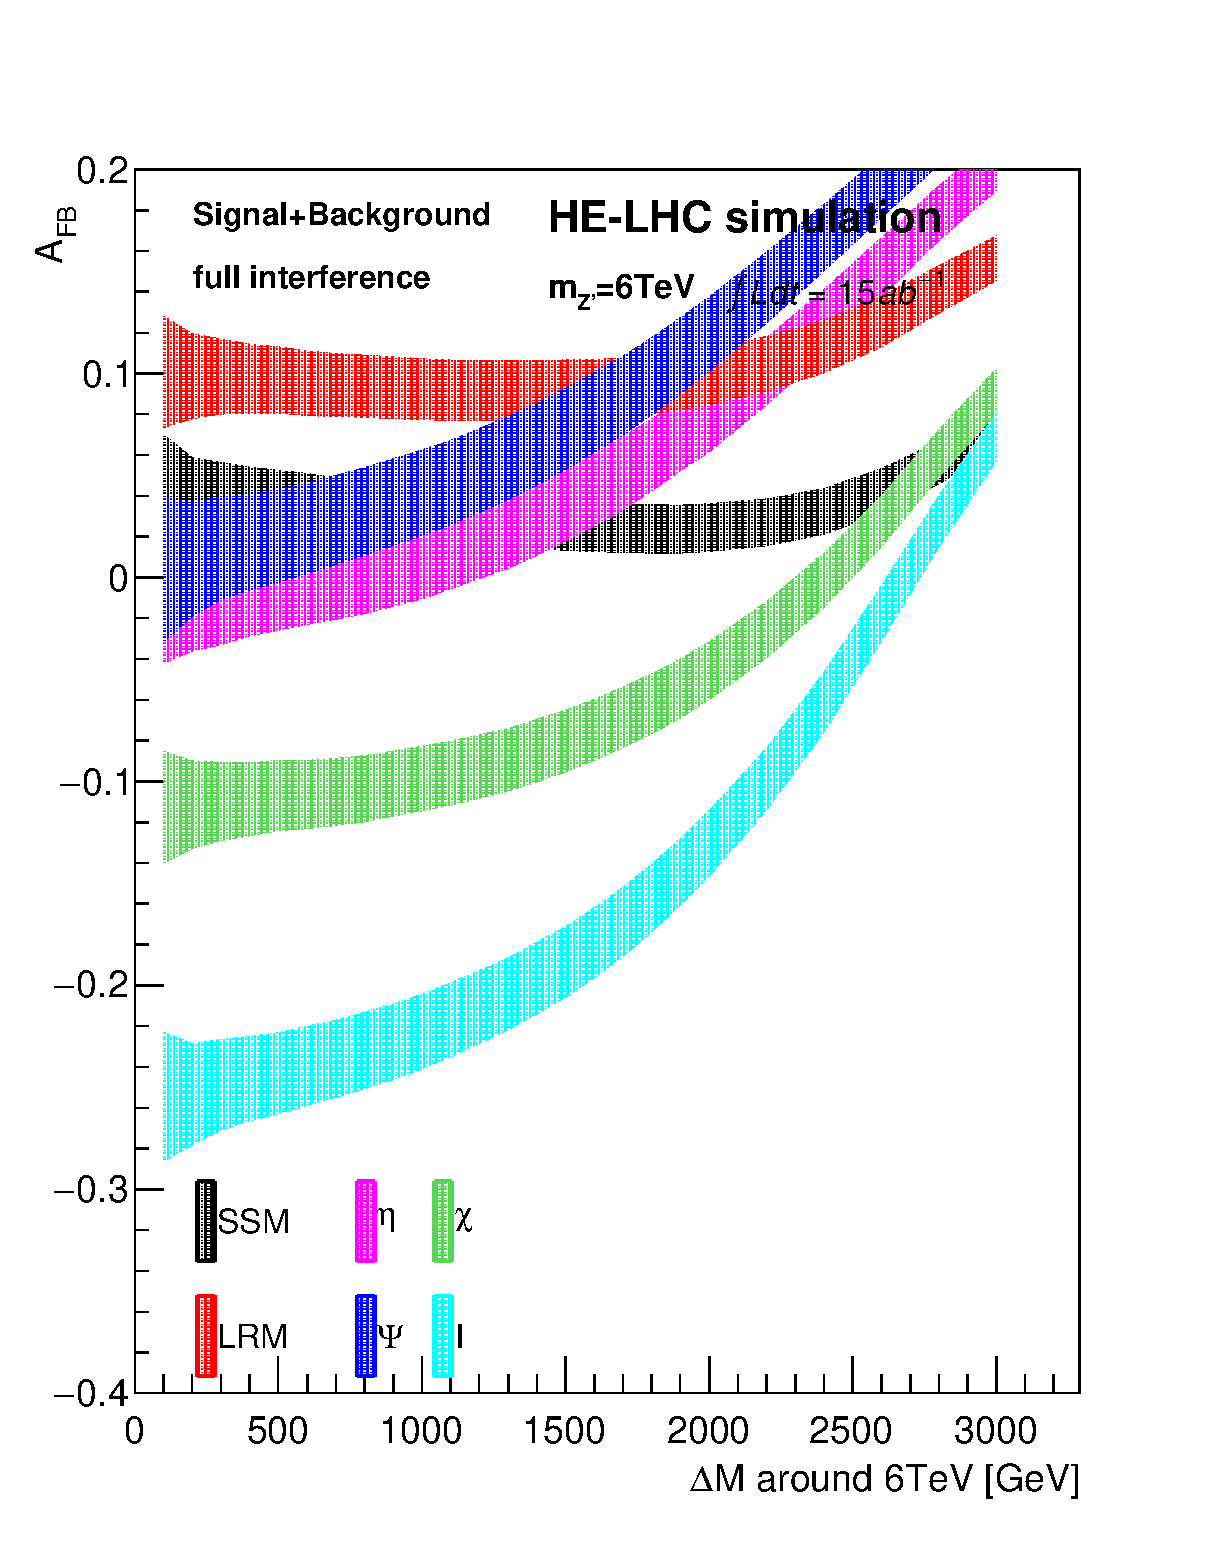
\includegraphics[width=0.45\columnwidth]{Fig/27tev/afb_vs_dm_interf.eps}
  \caption{$A_{FB}$ versus invariant mass range around 6TeV considering no backgrounds (top left), backgrounds with no uncertainties (top right), backgrounds with 10\% uncertainties (bottom left) and full interference (bottom right).}
  \label{figure:lepana:afb_dm}
\end{figure}

\noindent In Figure~\ref{figure:lepana:afb_bgerr} is represented the error on $A_{FB}$ verus the uncertainty on the Drell-Yan normalisation for different mass window around the 6~TeV signal.
The full dots represents the error on $A_{FB}$ when interference is considered. As expected from adding statistics, the larger the mass window, the smaller the error on $A_{FB}$ is. But this is 
only true when the uncertainty on the Drell-Yan is small. The other interesting effect can be seen when the mass window is small, leading to very little background contamination, thus the error on 
$A_{FB}$ increases extremely slowly with the uncertainty on the Drell-Yan, which tells us that when using a small mass, the measurement becomes transparent to uncertainty on the Drell-Yan.


\begin{figure}[!htb]
  \centering
   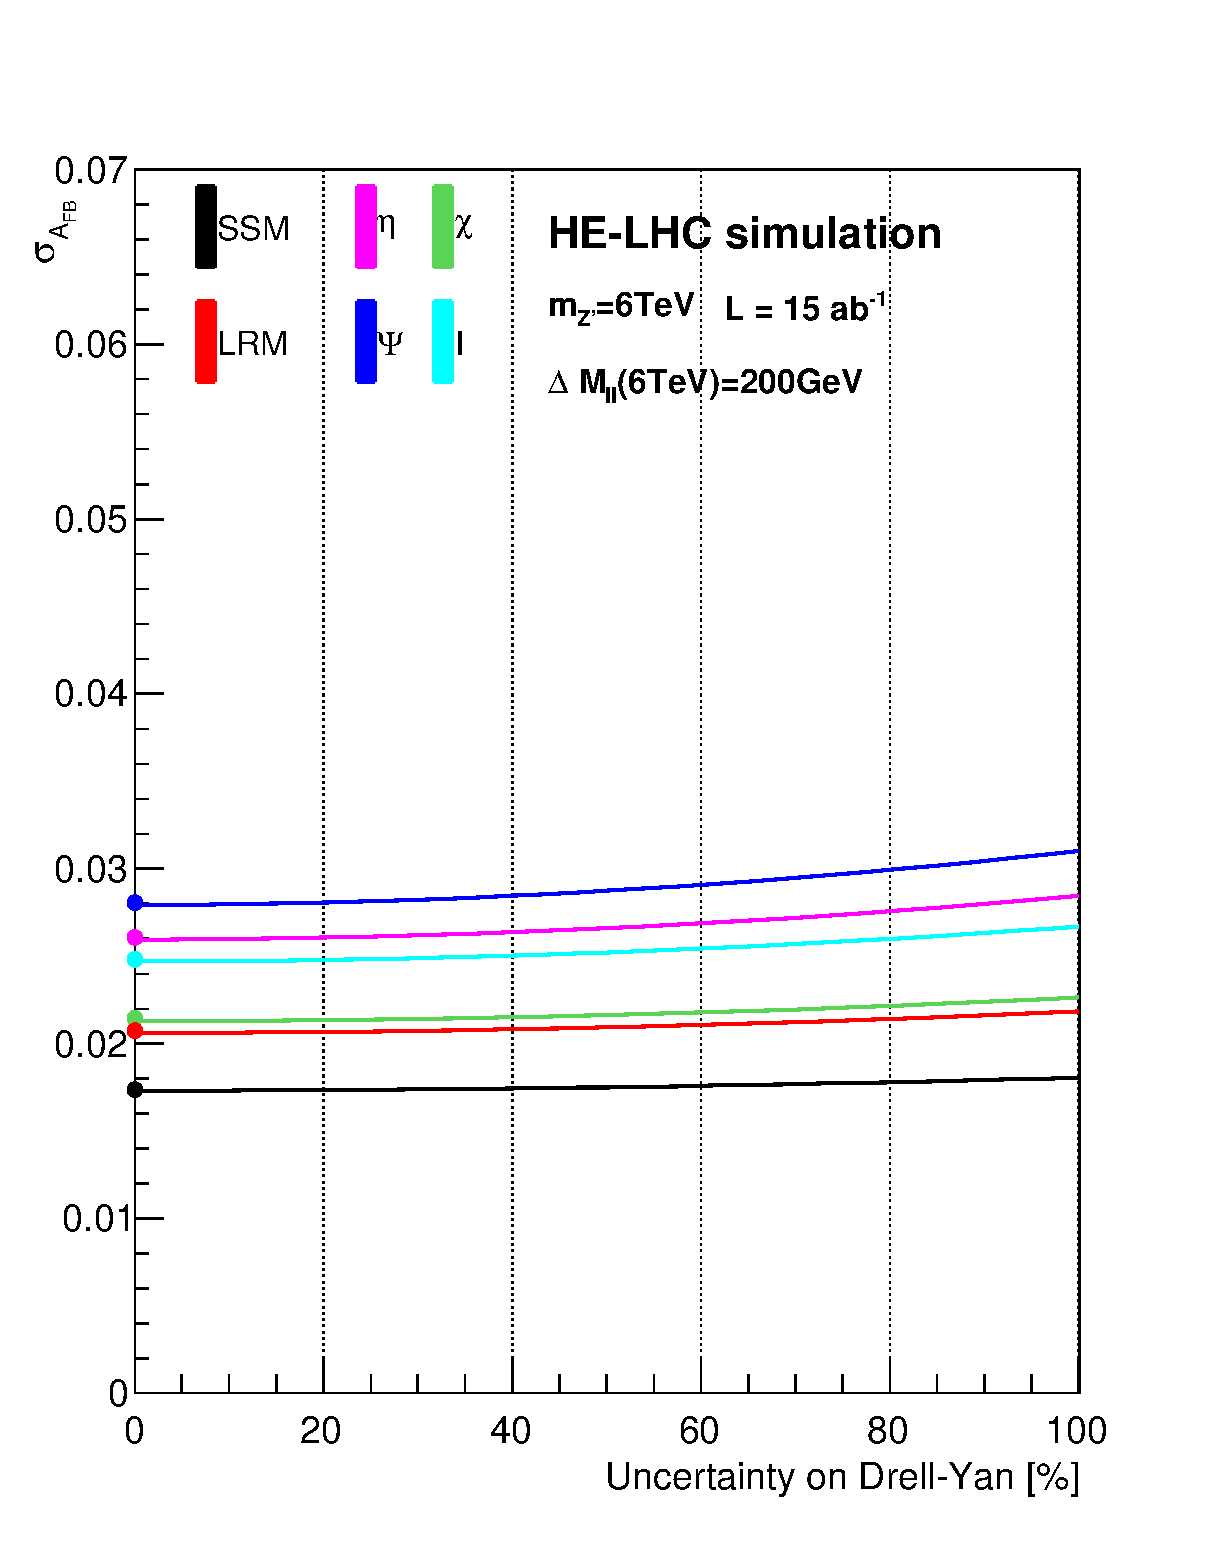
\includegraphics[width=0.45\columnwidth]{Fig/27tev/afb_vs_bgerr_200.eps}
   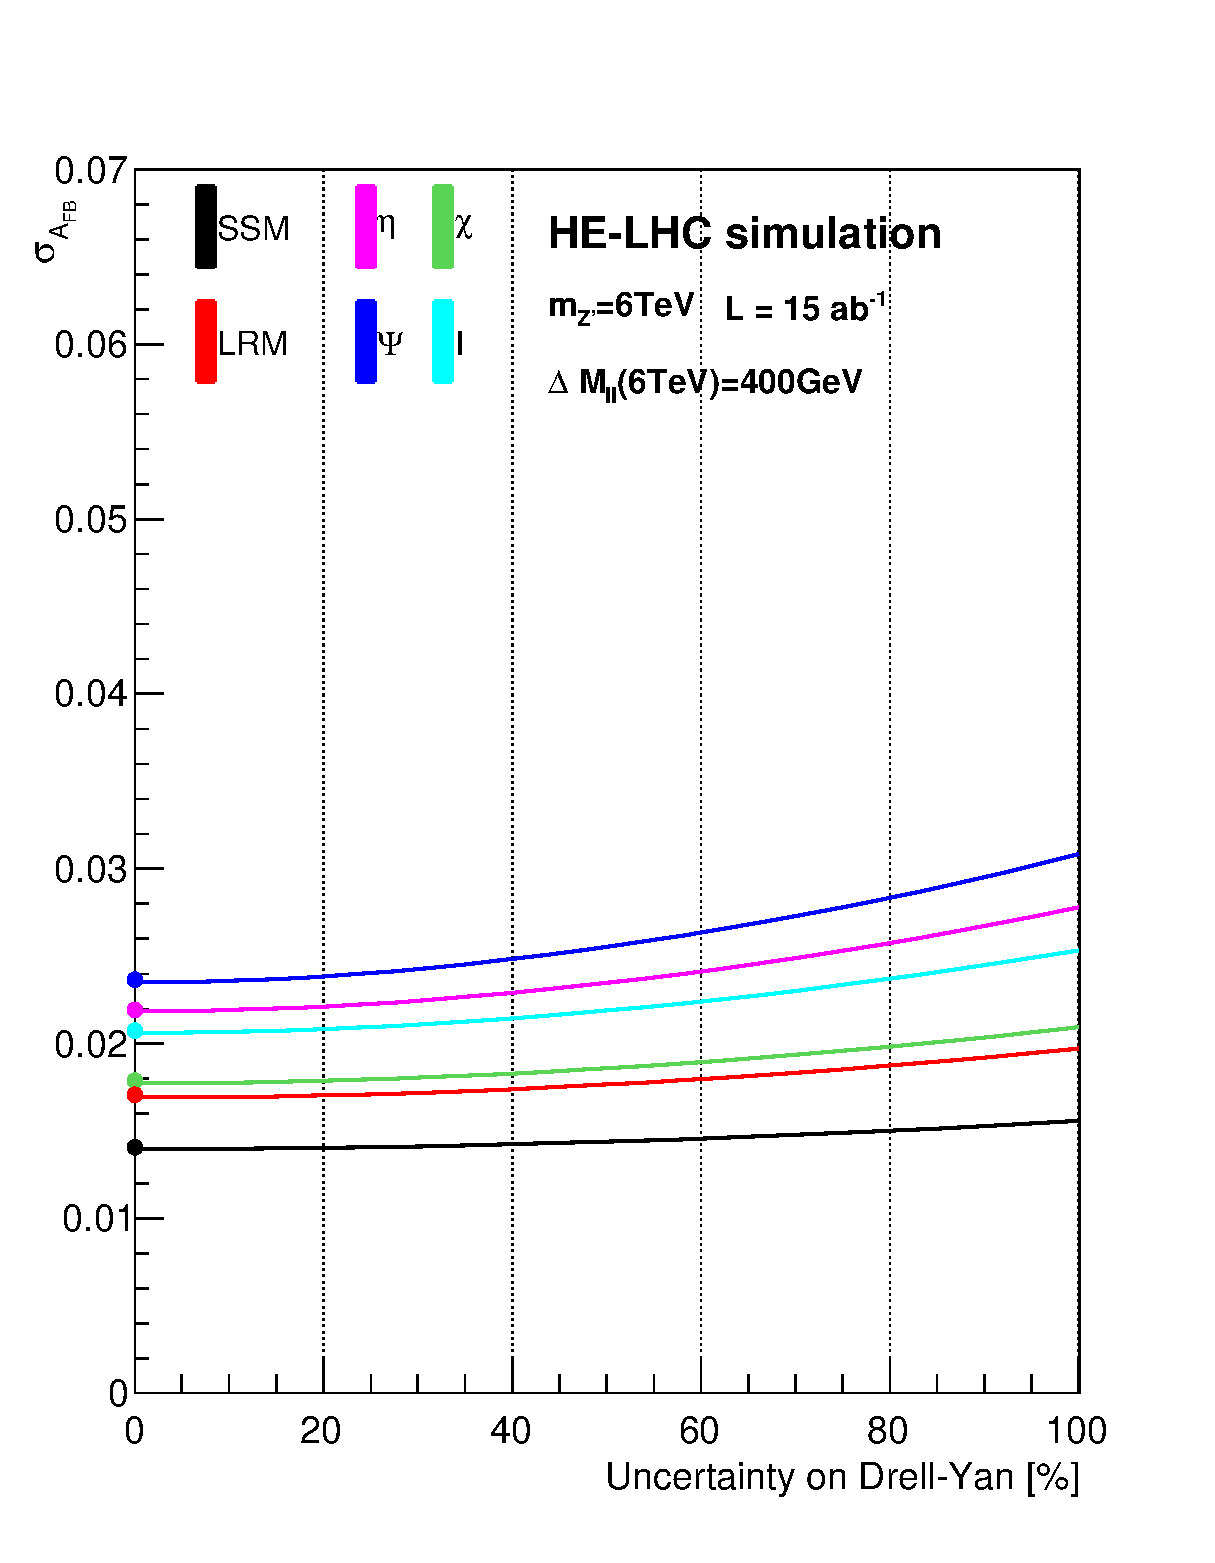
\includegraphics[width=0.45\columnwidth]{Fig/27tev/afb_vs_bgerr_400.eps}
   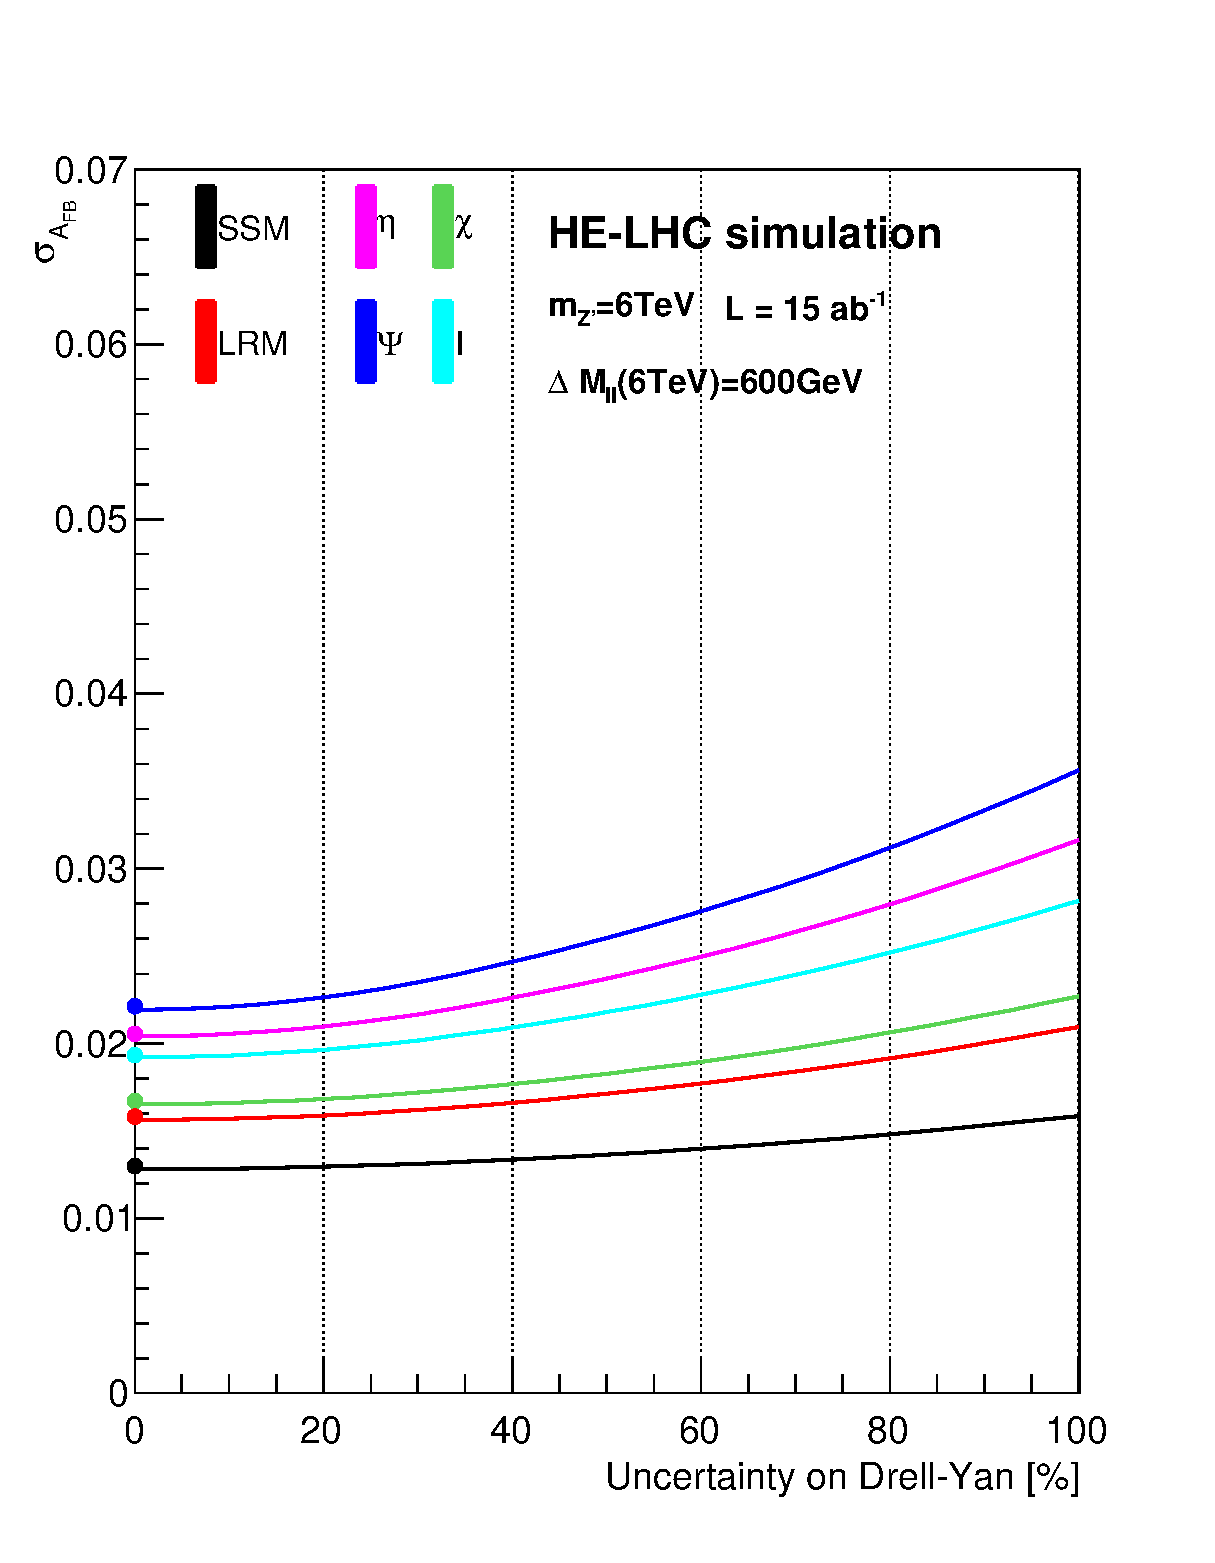
\includegraphics[width=0.45\columnwidth]{Fig/27tev/afb_vs_bgerr_600.eps}
   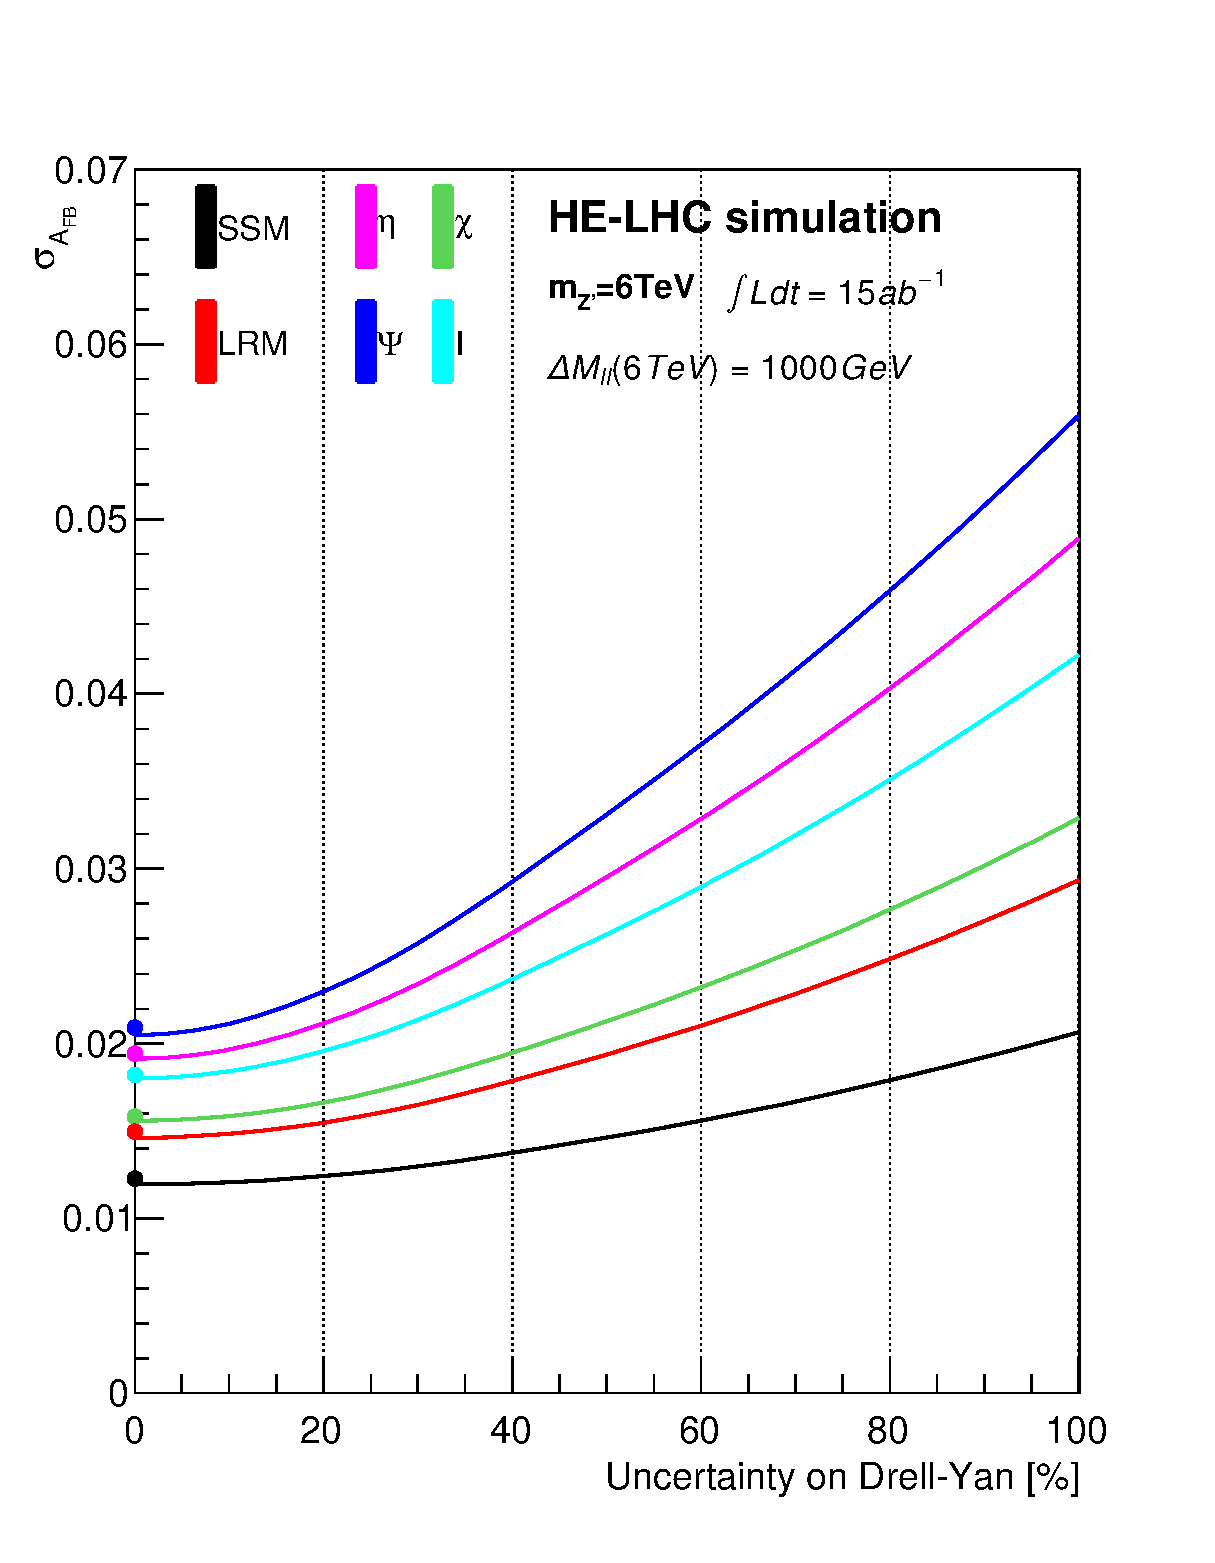
\includegraphics[width=0.45\columnwidth]{Fig/27tev/afb_vs_bgerr_1000.eps}
  \caption{Error on $A_{FB}$ versus uncertainty on the Drell-Yan normalisation for an invariant mass range around 6TeV of 200~GeV (top left),  400~GeV (top right), 600~GeV (bottom left) and 1000~GeV (bottom right).}
  \label{figure:lepana:afb_bgerr}
\end{figure}

\noindent In Table~\ref{tab:leptonicresonances:comp1} the values of $A_{FB}$ and $r_y$ for the different models considered together with their corresponding uncertainties for an integrated luminosity of 15~ab$^{-1}$ are shown. 
It is calculated for two different lepton acceptance, LHC-like acceptance $|\eta_l|<2.5$ and an increase coverage up to $|\eta_l|<4.5$. A small reduction in the error, mostly for $r_y$ is observed when considering a larger acceptance.

\begin{table}
\caption{$A_{FB}$ and $r_y$ values for different models and different lepton acceptance considering a mass window of 200~GeV. Uncertainties are show for an integrated luminosity of 15~ab$^{-1}$.}

\centering
\begin{tabular}{| c | c | c | c | c | c | |} 
\hline\hline
 & \multicolumn{2}{c|}{$|\eta_l|<2.5$}  & \multicolumn{2}{c|}{$|\eta_l|<4.5$} \\

\hline
  Model &  $A_{FB}$            &  $r_y$                  &  $A_{FB}$             &  $r_y$                 \\
\hline
SSM    &  0.045$\pm$0.017 & 1.96$\pm$0.072  & 0.046$\pm$0.017 & 1.85$\pm$0.066   \\
LRM    &  0.098$\pm$0.021 & 1.99$\pm$0.087  & 0.101$\pm$0.020 & 1.88$\pm$0.080   \\
$\psi$  &  0.001$\pm$0.028  & 1.96$\pm$0.118 & 0.000$\pm$0.028 & 1.85$\pm$0.107    \\
$\chi$  & -0.120$\pm$0.021  & 2.04$\pm$0.093 & -0.120$\pm$0.021 & 1.93$\pm$0.084   \\
$\eta$  & -0.224$\pm$0.026  & 1.95$\pm$0.109 & -0.023$\pm$0.026 & 1.84$\pm$0.099   \\
~I         & -0.260$\pm$0.025 & 2.17$\pm$0.113  & -0.262$\pm$0.024 & 2.04$\pm$0.103   \\
\hline\hline
\end{tabular}
\label{tab:leptonicresonances:comp1}
\end{table}

\noindent In Table~\ref{tab:leptonicresonances:comp2} the values of $A_{FB}$ and $r_y$ for the different models considered together with their corresponding statistical uncertainties are shown. 
It is calculated for two different cases, no final state radiations, and no initial nor final state radiations. This demonstrate that the measurement is little affected such effect.

\begin{table}
\caption{$A_{FB}$ and $r_y$ values for different models and removing ISR only and both ISR/FSR considering a mass window of 200~GeV. Uncertainties are of statistical nature only.}

\centering
\begin{tabular}{| c | c | c | c | c | c |} \hline\hline
 & \multicolumn{2}{c|}{no FSR} & \multicolumn{2}{c|}{no ISR/FSR}\\

\hline
  Model &  $A_{FB}$                &  $r_y$                    &  $A_{FB}$   &  $r_y$      \\
\hline
SSM    &   0.044$\pm$0.002    &  1.85$\pm$0.008  &  0.046$\pm$0.002  &  1.80$\pm$0.010   \\
LRM    &   0.098$\pm$0.002    &  1.88$\pm$ 0.008 &  0.102$\pm$0.002  &  1.85$\pm$0.009 \\
$\psi$  &   0.000$\pm$0.001    &  1.83$\pm$ 0.007 &   0.001$\pm$0.002 &  1.78$\pm$0.008\\
$\chi$  &   -0.118$\pm$0.002   &  1.92 $\pm$0.008 &  -0.129$\pm$0.002 &  1.92$\pm$0.009\\
$\eta$  &   -0.022$\pm$0.001  & 1.82$\pm$0.007   &  -0.023$\pm$0.002 &  1.76$\pm$0.008 \\
~I         &   -0.259$\pm$0.002  &  2.02$\pm$0.008  &   -0.288$\pm$0.002 &  2.04$\pm$0.010\\
\hline\hline
\end{tabular}
\label{tab:leptonicresonances:comp2}
\end{table}

%\noindent From the optimisation presented above, the results in the following section will be presented both with and without considering the interference.



\subsubsubsection{Results}
\label{subsubsection:results}

Figure~\ref{figure:lepana:afb_ry} represents the discrimination potential of $r_y$ and $A_{FB}$ together in different configurations. The two models $\chi$ and $I$ presents excellent discrimination while for SSM and LRM 
the differences are reduced. On the other hand, $\eta$ and $\Psi$ are almost fully degenerated.  


\begin{figure}[!htb]
  \centering
   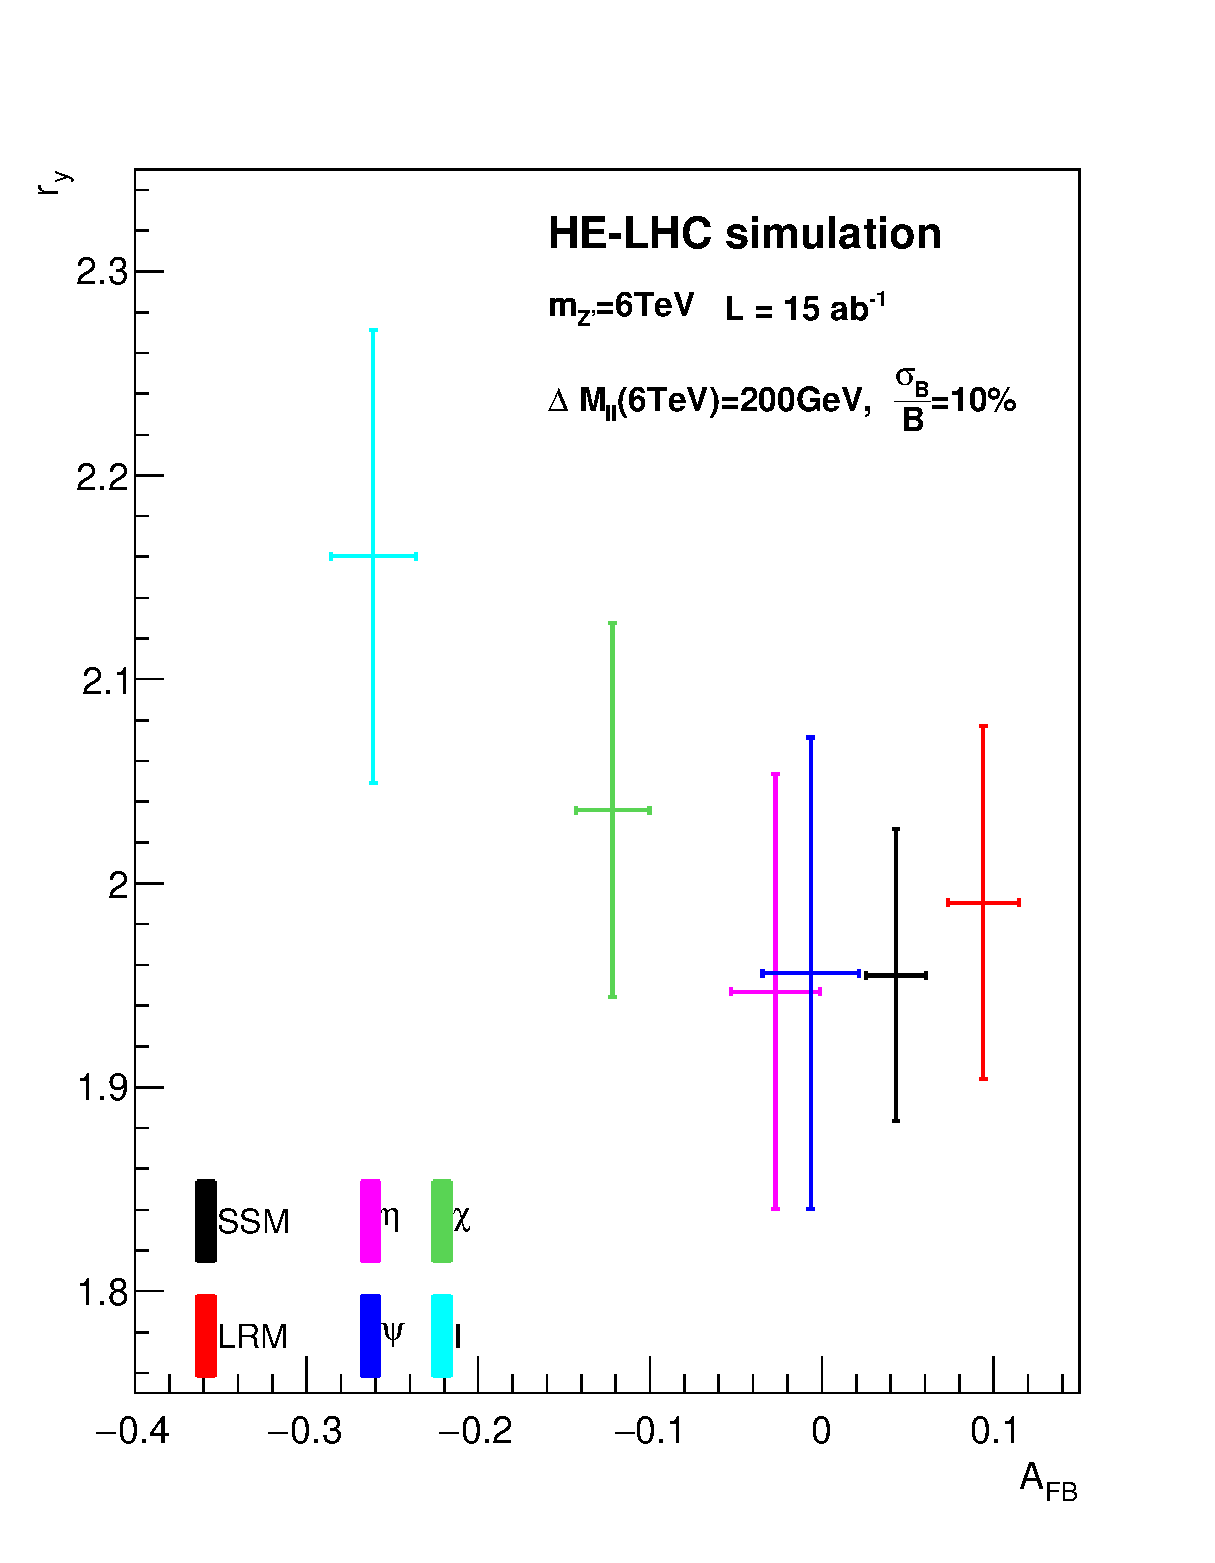
\includegraphics[width=0.45\columnwidth]{Fig/27tev/ry_afb_200GeV_eta2p5.eps}
   \includegraphics[width=0.45\columnwidth]{Fig/27tev/ry_afb_200GeV_eta2p5_interf.eps}
   \includegraphics[width=0.45\columnwidth]{Fig/27tev/ry_afb_500GeV_eta2p5.eps}
   \includegraphics[width=0.45\columnwidth]{Fig/27tev/ry_afb_500GeV_eta2p5_interf.eps}
  \caption{Scatter plot of $r_y$ versus $A_{FB}$ for 200(500)~GeV and mass window top(bottom). A 10\% uncertainty on the Drell-Yan is considered for the left plots while the full interference is shown on the right.}
  \label{figure:lepana:afb_ry}
\end{figure}

Using a profile likelihood technique, the signal strength $\mu$ can be fitted together with its corresponding error. Figure~\ref{figure:lepana:sigma_vs_lumi} represents this and it is on its own very discriminant, and 
it seems to be possible to even discriminate the previous two models that were not distinguishable. A side note, since the cross-section can easily be modified by just adding an overall rescaling of the coupling, 
it is clear it is not correct to claim discrimination just out of the cross-section.

\begin{figure}[!htb]
  \centering
   \includegraphics[width=0.45\columnwidth]{Fig/27tev/sigma.eps}
    \caption{Fitted signal cross-section together with its corresponding error versus integrated luminosity.}
  \label{figure:lepana:sigma_vs_lumi}
\end{figure}


\subsubsection{Hadronic analysis}
\label{subsection:hadana}
In this section the hadronic decays of the $Z'$ will be tested in order to enhance the discrimination potential. The event selection for the three considered hadronic decays in order 
to ensure excellent orthogonality is explained below. 

\subparagraph{$Z' \rightarrow t\bar{t}$}
The analysis presented in~\ref{subsec:hadreso} is used as baseline, with some modifications of the cuts explained in~\ref{sec:ana27tev}.
\subparagraph{$Z' \rightarrow b\bar{b}$}
This analysis selects two high $p_T$ b-tagged jets and veto events that have at least one top-tagged jets from $Z' \rightarrow t\bar{t}$ analysis.
\subparagraph{$Z' \rightarrow q\bar{q}$}
This analysis selects two high $p_T$  jets and veto events that have at least one top-tagged or b-tagged jets from $Z' \rightarrow t\bar{t}$ and $Z' \rightarrow b\bar{b}$ analyses.
Invariant mass of the di-jet system is shown on Figure~\ref{figure:hadronicresonances:masses}.

\begin{figure}[h]
  \centering
  \includegraphics[width=0.30\columnwidth]{Fig/27tev/Mj1j2_pf08_MetCorr_fit_sel0_nostack_log_tt.eps}
  \includegraphics[width=0.30\columnwidth]{Fig/27tev/Mj1j2_pf08_MetCorr_fit_sel0_nostack_log_bb.eps}
  \includegraphics[width=0.30\columnwidth]{Fig/27tev/Mj1j2_pf08_MetCorr_fit_sel0_nostack_log_jj.eps}
  \caption{Invariant mass for a 6~TeV signal after full event selection for $t\bar{t}$ channel (left), $b\bar{b}$ channel (center) and $q\bar{q}$ channel (right). }
  \label{figure:hadronicresonances:masses}
\end{figure}

\subsubsubsection{Results}
Figure~\ref{figure:hadana:discri30ab} summarise the discrimination potential in terms of fitted cross-section of the different models considering the three hadronic decays, $t\bar{t}$,  $b\bar{b}$ and $q\bar{q}$. 
Overall good discrimination can be reached, but nevertheless $\eta$ and $\Psi$ still presents similar results, except maybe for $t\bar{t}$ where some difference can be observed.


\begin{figure}[h]
  \centering
%    \includegraphics[width=0.3\columnwidth]{Fig/27tev/Zp_branching_4TeV_5ab.eps}
 %   \includegraphics[width=0.3\columnwidth]{Fig/27tev/Zp_branching_6TeV_5ab.eps}
 %   \includegraphics[width=0.3\columnwidth]{Fig/27tev/Zp_branching_8TeV_5ab.eps}

 %   \includegraphics[width=0.3\columnwidth]{Fig/27tev/Zp_branching_4TeV_15ab.eps}
    \includegraphics[width=0.45\columnwidth]{Fig/27tev/Zp_branching_6TeV_15ab.eps}
 %   \includegraphics[width=0.3\columnwidth]{Fig/27tev/Zp_branching_8TeV_15ab.eps}

  %  \includegraphics[width=0.3\columnwidth]{Fig/27tev/Zp_branching_4TeV_30ab.eps}
  %  \includegraphics[width=0.3\columnwidth]{Fig/27tev/Zp_branching_6TeV_30ab.eps}
  %  \includegraphics[width=0.3\columnwidth]{Fig/27tev/Zp_branching_8TeV_30ab.eps}
    \caption{Fitted cross-section of the three hadronic analyses. Statistical and full uncertainties are shown on each point.}

  \label{figure:hadana:discri30ab}
\end{figure}

The model discrimination achieved by the hadronic analyses for 4, 6 and 8TeV considering an integrated luminosity of 
5, 15 and 30ab$^{-1}$ respectively is shown on Fig.~\ref{figure:hadana:discri5ab}, \ref{figure:hadana:discri15ab}, \ref{figure:hadana:discri30ab}.
From the leptonic analysis~\ref{sec:lepana}, it was shown that for $r_y$ 
For all cases, except for a mass of 8TeV and an integrated luminosity of 5ab$^{-1}$, discrimination is obtained at more than one sigma for the di-jet case.


\subsection{Summary}


%%%%%%%%%%%%%%%%%%%%%%%%%%%%%%%%%%%%%%%%%%%%%%%%%%%%%
\section{Conclusion}
This note presents preliminary studies of a search for $\Zp$ 
bosons decaying into two electrons or muons in the FCC context. The expected number 
of signal and background events have been estimated from simulated truth level information 
after applying smearing functions to mimic the FCC detector response.
Using a cut-based analysis and assuming simplistic systematic uncertainties, $\ZpSSM$
masses below 40 $\TeV$ can be excluded at 95$\%$ C.L. 
using 30 $\afb{}$ of data. 
\clearpage
\newpage

%%%%%%%%%%%%%%%%%%%%%%%%%%%%%%%%%%%%%%%%%%%%%%%%%%%%%
%%%%%%%%%%%%%%%%%%%%%%%%%%%%%%%%%%%%%%%%%%%%%%%%%%%%%
\appendix
%%%%%%%%%%%%%%%%%%%%%%%%%%%%%%%%%%%%%%%%%%%%%%%%%%%%%
%%%%%%%%%%%%%%%%%%%%%%%%%%%%%%%%%%%%%%%%%%%%%%%%%%%%%
\section{ Appendix : TMVA}
\label{appendix:tmva}

\begin{figure}[!htb]\centering
\includegraphics[width=0.9\textwidth]{Fig/TMVA/thad_vs_QCD/variables_id_c1.eps}
\includegraphics[width=0.9\textwidth,trim={0 5cm 0 0},clip]{Fig/TMVA/thad_vs_QCD/variables_id_c2.eps}
\caption{Input variables for top Vs QCD tagger.}
\label{fig:TMVA_inputs_t}
\end{figure}

\begin{figure}[!htb]\centering
\includegraphics[width=0.9\textwidth]{Fig/TMVA/Whad_vs_QCD/variables_id_c1.eps}
\includegraphics[width=0.9\textwidth]{Fig/TMVA/Whad_vs_QCD/variables_id_c2.eps}
\includegraphics[width=0.9\textwidth,trim={0 5cm 0 0},clip]{Fig/TMVA/Whad_vs_QCD/variables_id_c3.eps}
\caption{Input variables for W Vs QCD tagger.}
\label{fig:TMVA_inputs_w}
\end{figure}

\begin{figure}[!htb]\centering
\includegraphics[width=0.495\textwidth]{Fig/TMVA/thad_vs_QCD/CorrelationMatrixS.eps}
\includegraphics[width=0.495\textwidth]{Fig/TMVA/thad_vs_QCD/CorrelationMatrixB.eps}
\includegraphics[width=0.495\textwidth]{Fig/TMVA/Whad_vs_QCD/CorrelationMatrixS.eps}
\includegraphics[width=0.495\textwidth]{Fig/TMVA/Whad_vs_QCD/CorrelationMatrixB.eps}
\caption{Correlation matrices for Signal (left) and Background (right) for top Vs QCD tagger (top) and W Vs QCD tagger (bottom).}
\label{fig:TMVA_corr_matrix}
\end{figure}

\begin{figure}[!htb]\centering
\includegraphics[width=0.495\textwidth]{Fig/TMVA/thad_vs_QCD/overtrain_BDT_thad_vs_QCD.eps}
\includegraphics[width=0.495\textwidth]{Fig/TMVA/Whad_vs_QCD/overtrain_BDT_Whad_vs_QCD.eps}
\caption{BDT scores for Signal (red) and Background (blue) for top Vs QCD tagger (left) and W Vs QCD tagger (right).}
\label{fig:TMVA_BDTscore}
\end{figure}

\begin{figure}[!htb]\centering
\includegraphics[width=0.495\textwidth]{Fig/TMVA/thad_vs_QCD/rejBvsS.eps}
\includegraphics[width=0.495\textwidth]{Fig/TMVA/Whad_vs_QCD/rejBvsS.eps}
\caption{Top ROC curves show background rejection Vs Signal efficiency for top Vs QCD tagger (left) and W Vs QCD tagger (right).}
\label{fig:TMVA_ROC}
\end{figure}

\begin{figure}[!htb]\centering
\includegraphics[width=0.495\textwidth]{Fig/TMVA/Jet1_thad_vs_QCD_tagger.eps}
\includegraphics[width=0.495\textwidth]{Fig/TMVA/Jet2_thad_vs_QCD_tagger.eps}
\includegraphics[width=0.495\textwidth]{Fig/TMVA/Jet1_Whad_vs_QCD_tagger.eps}
\includegraphics[width=0.495\textwidth]{Fig/TMVA/Jet2_Whad_vs_QCD_tagger.eps}
\caption{Signal BDT score shapes comparison for masses from 10 to 35 $\TeV$ (and ratio to 20 $\TeV$ mass) for leading jet (left) and second leading jet $\pt$ (right) for top Vs QCD tagger (top) and W Vs QCD tagger (bottom).}
\label{fig:BDT_signal_shape_comparison}
\end{figure}

\clearpage
\newpage

%%%%%%%%%%%%%%%%%%%%%%%%%%%%%%%%%%%%%%%%%%%%%%%%%%%%%
%%%%%%%%%%%%%%%%%%%%%%%%%%%%%%%%%%%%%%%%%%%%%%%%%%%%%
\section{Appendix : \zptt\ 100 TeV}
\label{appendix:zptt100}

% useless
%\begin{figure}[!htb]\centering
%\includegraphics[width=0.8\textwidth]{Fig/Zptt/rapiditySeparation_sel0_before_cut_nostack_log.eps}
%\caption{Rapidity separation at preselection level before cut on this variable in \zptt\ analysis. The generated mass of the signal sample is 10 $\TeV$.}
%\label{fig:Zptt_sel0_rapidity}
%\end{figure}

\begin{figure}[!htb]\centering
\includegraphics[width=0.32\textwidth]{Fig/Zptt/Jet1_trk02_SD_Cor_m_sel0_nostack_log.eps}
\includegraphics[width=0.32\textwidth]{Fig/Zptt/Jet1_tau21_sel0_nostack_log.eps}
\includegraphics[width=0.32\textwidth]{Fig/Zptt/Jet1_tau32_sel0_nostack_log.eps}
\caption{Variables used for the first step of cuts in cut-based analysis at preselection level for leading jet $\pT$ in \zptt\ analysis : jet mass SD (Soft-Dropped) corrected, jet $\tau_{21}$ and jet $\tau_{32}$. The generated mass of the signal sample is 10 $\TeV$.}
\label{fig:Zptt_sel0_cut}
\end{figure}

\begin{figure}[!htb]\centering
\includegraphics[width=0.32\textwidth]{Fig/Zptt/Jet2_trk02_SD_Cor_m_sel1_nostack_log.eps}
\includegraphics[width=0.32\textwidth]{Fig/Zptt/Jet2_tau21_sel1_nostack_log.eps}
\includegraphics[width=0.32\textwidth]{Fig/Zptt/Jet2_tau32_sel1_nostack_log.eps}
\caption{Variables used for the second step of cuts in cut-based analysis after first set of cuts for second leading jet $\pT$ in \zptt\ analysis : jet mass SD (Soft-Dropped) corrected, jet $\tau_{21}$ and jet $\tau_{32}$. The generated mass of the signal sample is 10 $\TeV$.}
\label{fig:Zptt_sel1_cut}
\end{figure}

\begin{figure}[!htb]\centering
\includegraphics[width=0.32\textwidth]{Fig/Zptt/Jet1_thad_vs_QCD_tagger_sel0_nostack_log.eps}
\includegraphics[width=0.32\textwidth]{Fig/Zptt/Jet2_thad_vs_QCD_tagger_sel0_nostack_log.eps}
\caption{top Vs QCD tagger at preselection level for leading jet (left) and second leading jet $\pT$ (right) in \zptt\ analysis. The generated mass of the signal sample is 10 $\TeV$.}
\label{fig:Zptt_sel0_tagger}
\end{figure}

\begin{figure}[!htb]\centering
\includegraphics[width=0.32\textwidth]{Fig/Zptt/Jet1_trk02_SD_Cor_m_sel3_nostack_log.eps}
\includegraphics[width=0.32\textwidth]{Fig/Zptt/Jet2_trk02_SD_Cor_m_sel3_nostack_log.eps}
\caption{Jet mass SD (Soft-Dropped) corrected in anti-QCD tagger-based analysis after first set of cuts for leading jet (left) and second leading jet $\pT$ (right) in \zptt\ analysis. The generated mass of the signal sample is 10 $\TeV$.}
\label{fig:Zptt_sel1_tagger}
\end{figure}

% no eps -> useless
%\begin{figure}[!htb]\centering
%\includegraphics[width=0.33\textwidth]{Fig/check_TRF/Zptt/jet12pdgID_QCD5f_redModule_blueDELPHES.png}
%\includegraphics[width=0.33\textwidth]{Fig/check_TRF/Zptt/jet12pdgID_ttbar_redModule_blueDELPHES.png}
%\includegraphics[width=0.33\textwidth]{Fig/check_TRF/Zptt/jet12pdgID_Zptt10TeV_redModule_blueDELPHES.png}
%\includegraphics[width=0.33\textwidth]{Fig/check_TRF/Zptt/TRF2tagex_module_redZptt10TeV_blackQCD_bluettbar.png}
%\caption{Checks of pdgID obtained from recomputation (red) compared to Delphes information (blue) for leading jet (continuous line) and second leading jet $\pT$ (dashed line), and for QCD (top left), $\ttbar$ (top right) and \zptt\ 10 $\TeV$ (bottom left) samples in \zptt\ analysis. Tag Rate Function for a two b-tagged jets event computed from the two leading jets only of the event (bottom right) for QCD (black), $\ttbar$ blue) and \zptt\ 10 $\TeV$ (red) samples.}
%\label{fig:Zptt_TRFchecks}
%\end{figure}

% no eps -> useless
%\begin{figure}[!htb]\centering
%\includegraphics[width=0.33\textwidth]{Fig/check_TRF/tth_boosted/jet12pdgID_ttbb_redModule_blueDELPHES.png}
%\includegraphics[width=0.33\textwidth]{Fig/check_TRF/tth_boosted/jet12pdgID_ttj_redModule_blueDELPHES.png}
%\includegraphics[width=0.33\textwidth]{Fig/check_TRF/tth_boosted/jet12pdgID_ttz_redModule_blueDELPHES.png}
%\includegraphics[width=0.33\textwidth]{Fig/check_TRF/tth_boosted/jet12pdgID_tth_redModule_blueDELPHES.png}
%\caption{Checks of pdgID obtained from recomputation (red) compared to Delphes information (blue) for leading jet (continuous line) and second leading jet $\pT$ (dashed line), and for $\ttbb$ (top left), $\ttj$ (top right), $\ttz$ (bottom left) and $\tthbb$ (bottom right) samples in $\tthbb$ boosted analysis.}
%\label{fig:tthboosted_TRFchecks1}
%\end{figure}

% no eps -> useless
%\begin{figure}[!htb]\centering
%\includegraphics[width=0.33\textwidth]{Fig/check_TRF/tth_boosted/jet34pdgID_ttbb_redModule_blueDELPHES.png}
%\includegraphics[width=0.33\textwidth]{Fig/check_TRF/tth_boosted/jet34pdgID_ttj_redModule_blueDELPHES.png}
%\includegraphics[width=0.33\textwidth]{Fig/check_TRF/tth_boosted/jet34pdgID_ttz_redModule_blueDELPHES.png}
%\includegraphics[width=0.33\textwidth]{Fig/check_TRF/tth_boosted/jet34pdgID_tth_redModule_blueDELPHES.png}
%\caption{Checks of pdgID obtained from recomputation (red) compared to Delphes information (blue) for third leading jet (continuous line) and fourth leading jet $\pT$ (dashed line), and for $\ttbb$ (top left), $\ttj$ (top right), $\ttz$ (bottom left) and $\tthbb$ (bottom right) samples in $\tthbb$ boosted analysis.}
%\label{fig:tthboosted_TRFchecks2}
%\end{figure}

% -> useless
%\begin{figure}[!htb]\centering
%\includegraphics[width=0.495\textwidth]{Fig/Zptt/Mj1j2_pf08_MetCorr_fit_sel2_nostack_log.eps}
%\includegraphics[width=0.495\textwidth]{Fig/Zptt/Mj1j2_pf08_MetCorr_fit_sel4_nostack_log.eps}
%\includegraphics[width=0.495\textwidth]{Fig/Zptt/Mj1j2_pf08_MetCorr_fit_sel5_nostack_log.eps}
%\includegraphics[width=0.495\textwidth]{Fig/Zptt/Mj1j2_pf08_MetCorr_fit_sel6_nostack_log.eps}
%\includegraphics[width=0.495\textwidth]{Fig/Zptt/Mj1j2_pf08_MetCorr_fit_sel7_nostack_log.eps}
%\includegraphics[width=0.495\textwidth]{Fig/Zptt/Mj1j2_pf08_MetCorr_fit_sel8_nostack_log.eps}
%\caption{Zprime mass after the full selection for anaylsis cut-based (left) and anti-QCD tagger based (right), and for the b-tagging scenarios : before b-tag (top), direct 2 b-tag (middle) and Tag Rate Function 2 b-tag (bottom) in \zptt\ analysis. The generated mass of the signal sample is 10 $\TeV$.}
%\label{fig:Zptt_mass_sel_final}
%\end{figure}

%  -> useless
%\begin{figure}[!htb]\centering
%\includegraphics[width=0.495\textwidth]{Fig/Zptt/lim_Zprime_tt_fcc_v02_cut.eps}
%\includegraphics[width=0.495\textwidth]{Fig/Zptt/DiscoveryPotential_tt_cut_rootStyle.eps}
%\includegraphics[width=0.495\textwidth]{Fig/Zptt/lim_Zprime_tt_fcc_v02_tagger.eps}
%\includegraphics[width=0.495\textwidth]{Fig/Zptt/DiscoveryPotential_tt_TC2_tagger_rootStyle.eps}
%\caption{Limit (left) and discovery potential (right) for analysis cut-based with direct b-tagging (top) and anti-QCD tagger-based with direct b-tagging (bottom) in \zptt\ analysis. Default model used for discovery potential is TC2.}
%\label{fig:Zptt_limit_direct}
%\end{figure}

\begin{figure}[!htb]\centering
\includegraphics[width=0.33\textwidth]{Fig/Zptt/lim_Zprime_tt_fcc_v02_cut_TRFbtag.eps}
\includegraphics[width=0.33\textwidth]{Fig/Zptt/DiscoveryPotential_tt_cut_TRFbtag_rootStyle.eps}
\includegraphics[width=0.33\textwidth]{Fig/Zptt/lim_Zprime_tt_fcc_v02_tagger_TRFbtag.eps}
\includegraphics[width=0.33\textwidth]{Fig/Zptt/DiscoveryPotential_tt_SSM_TC2_tagger_TRFbtag_rootStyle.eps}
\caption{Limit (left) and discovery potential (right) for analysis cut-based with TRF b-tagging (top) and anti-QCD tagger-based with TRF b-tagging (bottom) in \zptt\ analysis. Default model used for discovery potential is TC2 in the top plot. The bottom discovery plot shows the comparison between the TC2 default model (red line) and the SSM one (blue line).}
\label{fig:Zptt_limit_trf}
\end{figure}

%\begin{landscape}
\begin{table}[!htb]\centering
\scalebox{0.75}{
\begin{tabular}{|c|c|c|c|c|c|}
\hline
\hline
\multicolumn{2}{|c|}{}          & preselection                                                & cut1                                    & cut2                                    & btag                    \\
\hline
\multicolumn{2}{|c|}{selection} & $Jet_{1,2}^{trk02 SD Corr}~\pT$ > 3 TeV                     & preselection +                          & cut1 +                                  & cut2 +                  \\
\multicolumn{2}{|c|}{}          & |$Jet_{1,2}^{trk02 SD Corr}~\eta$| < 3                      & 0.3 < $Jet_{1}^{trk02}~\tau_{21}$ < 0.7 & 0.3 < $Jet_{2}^{trk02}~\tau_{21}$ < 0.7 & 2 TRF btag              \\
\multicolumn{2}{|c|}{}          & $Jet_{1,2}^{trk02}~\tau_{21,31,32}$ > 0                     & $Jet_{1}^{trk02}~\tau_{32}$ < 0.7       & $Jet_{2}^{trk02}~\tau_{32}$ < 0.75      & (on the 2 leading jets) \\
\multicolumn{2}{|c|}{}          & |$\Delta(Jet_{1}^{trk02}~\eta,Jet_{2}^{trk02}~\eta]$| < 2.4 & $Jet_{1}^{trk02 SD Corr}~M$ > 100 GeV   & $Jet_{2}^{trk02 SD Corr}~M$ > 100 GeV   &                         \\
\multicolumn{2}{|c|}{}          & $M_{Jet_{1},Jet_{2}}^{METcorr}$(pf08) > 5 GeV   &    &   & \\
\hline
\hline
background      & vv            & 41820     & 1470     & 33      & 1     \\
                & vj            & 1610472   & 70864    & 2390    & 5     \\
                & tt            & 1114779   & 472480   & 209660  & 54627 \\
                & QCD           & 154855591 & 16915581 & 2846240 & 10999 \\
                & Total         & 157622662 & 17460395 & 3058323 & 65632 \\
\hline
signal $m_{Z}$= & 10 TeV        & 101529    & 48916    & 27591   & 9278  \\
                & 15 TeV        & 31764     & 14769    & 7460    & 1876  \\
                & 20 TeV        & 7775      & 3561     & 1703    & 304   \\
                & 25 TeV        & 1926      & 867      & 402     & 50    \\
                & 30 TeV        & 485       & 216      & 98      & 9     \\
                & 35 TeV        & 124       & 54       & 25      & 2     \\
\hline
\hline
\end{tabular}}
\caption{Summary of \zptt\ analysis cut-flow for cut-based analysis.}
\label{tab:Zptt_cutflow_cut}
\end{table}
%\end{landscape}

%\begin{landscape}
\begin{table}[!htb]\centering
\scalebox{0.75}{
\begin{tabular}{|c|c|c|c|c|c|}
\hline
\hline
\multicolumn{2}{|c|}{}          & preselection & tagger1 & tagger2 & btag \\
\hline
\multicolumn{2}{|c|}{selection} & $Jet_{1,2}^{trk02 SD Corr}~\pT$ > 3 TeV                     & preselection +                  & tagger1 +                               & tagger2 +               \\
\multicolumn{2}{|c|}{}          & |$Jet_{1,2}^{trk02 SD Corr}~\eta$| < 3                      & $Jet_{1,2}~t/QCD tagger$ > 0.15 & $Jet_{1,2}^{trk02 SD Corr}~M$ > 40 GeV  & 2 TRF btag              \\
\multicolumn{2}{|c|}{}          & $Jet_{1,2}^{trk02}~\tau_{21,31,32}$ > 0                     &                                 &                                         & (on the 2 leading jets) \\
\multicolumn{2}{|c|}{}          & |$\Delta(Jet_{1}^{trk02}~\eta,Jet_{2}^{trk02}~\eta]$| < 2.4 &                                 &                                         &                          \\
\multicolumn{2}{|c|}{}          & $M_{Jet_{1},Jet_{2}}^{METcorr}$(pf08) > 5 GeV   &    &   &   \\
\hline
\hline
background      & vv            & 41820     & 7109    & 6998    & 17    \\
                & vj            & 1610472   & 107224  & 103958  & 264   \\
                & tt            & 1114779   & 257401  & 253907  & 74194 \\
                & QCD           & 154855591 & 2848680 & 2777145 & 11440 \\
                & Total         & 157622662 & 3220414 & 3142008 & 85915 \\
\hline
signal $m_{Z}$= & 10 TeV        & 101529    & 49199   & 48415   & 15602 \\
                & 15 TeV        & 31764     & 13255   & 12943   & 3306  \\
                & 20 TeV        & 7775      & 2594    & 2530    & 501   \\
                & 25 TeV        & 1926      & 491     & 480     & 76    \\
                & 30 TeV        & 485       & 97      & 95      & 13    \\
                & 35 TeV        & 124       & 21      & 21      & 3     \\
\hline
\hline
\end{tabular}}
\caption{Summary of \zptt\ analysis cut-flow for tagger-based analysis.}
\label{tab:Zptt_cutflow_tagger}
\end{table}
%\end{landscape}

\clearpage
\newpage

%%%%%%%%%%%%%%%%%%%%%%%%%%%%%%%%%%%%%%%%%%%%%%%%%%%%%
%%%%%%%%%%%%%%%%%%%%%%%%%%%%%%%%%%%%%%%%%%%%%%%%%%%%%
\section{Appendix : \rsg\ 100 TeV}
\label{appendix:rsg100}

%  -> useless
%\begin{figure}[!htb]\centering
%\includegraphics[width=0.8\textwidth]{Fig/RSGww/rapiditySeparation_sel0_before_cut_nostack_log.eps}
%\caption{Rapidity separation at preselection level before cut on this variable in \rsg\ analysis. The generated mass of the signal sample is 10 $\TeV$.}
%\label{fig:RSGww_sel0_rapidity}
%\end{figure}

\begin{figure}[!htb]\centering
\includegraphics[width=0.33\textwidth]{Fig/RSGww/Jet1_trk02_SD_Cor_m_sel0_nostack_log.eps}
\includegraphics[width=0.33\textwidth]{Fig/RSGww/Jet2_trk02_SD_Cor_m_sel0_nostack_log.eps}
\includegraphics[width=0.33\textwidth]{Fig/RSGww/Jet1_tau21_sel0_nostack_log.eps}
\includegraphics[width=0.33\textwidth]{Fig/RSGww/Jet2_tau21_sel0_nostack_log.eps}
\caption{Variables used for the first step of cuts in cut-based analysis at preselection level for leading jet (left) and second leading jet $\pT$ (right) in \rsg\ analysis : jet mass SD (Soft-Dropped) corrected (top) and jet $\tau_{21}$ (bottom). The generated mass of the signal sample is 10 $\TeV$.}
\label{fig:RSGww_sel0_cut}
\end{figure}

\begin{figure}[!htb]\centering
\includegraphics[width=0.33\textwidth]{Fig/RSGww/Jet1_Flow45_sel1_nostack_log.eps}
\includegraphics[width=0.33\textwidth]{Fig/RSGww/Jet2_Flow45_sel1_nostack_log.eps}
\includegraphics[width=0.33\textwidth]{Fig/RSGww/Jet1_Flow55_sel1_nostack_log.eps}
\includegraphics[width=0.33\textwidth]{Fig/RSGww/Jet2_Flow55_sel1_nostack_log.eps}
\caption{Variables used for the second step of cuts in cut-based analysis after first set of cuts for leading jet (left) and second leading jet $\pT$ (right) in \rsg\ analysis : jet Flow45 (top) and Flow55 (bottom). The generated mass of the signal sample is 10 $\TeV$.}
\label{fig:RSGww_sel1_cut}
\end{figure}

\begin{figure}[!htb]\centering
\includegraphics[width=0.33\textwidth]{Fig/RSGww/Jet1_Whad_vs_QCD_tagger_sel0_nostack_log.eps}
\includegraphics[width=0.33\textwidth]{Fig/RSGww/Jet2_Whad_vs_QCD_tagger_sel0_nostack_log.eps}
\caption{W Vs QCD tagger at preselection level for leading jet (left) and second leading jet $\pT$ (right) in \rsg\ analysis. The generated mass of the signal sample is 10 $\TeV$.}
\label{fig:RSGww_sel0_tagger}
\end{figure}

%  -> ugly
%\begin{figure}[!htb]\centering
%\includegraphics[width=0.33\textwidth]{Fig/RSGww/Jet1_trk02_SD_Cor_m_sel3_nostack_log.eps}
%\includegraphics[width=0.33\textwidth]{Fig/RSGww/Jet2_trk02_SD_Cor_m_sel3_nostack_log.eps}
%\caption{Jet mass SD (Soft-Dropped) corrected in anti-QCD tagger-based analysis after first set of cuts for leading jet (left) and second leading jet $\pT$ (right) in \rsg\ analysis. The generated mass of the signal sample is 10 $\TeV$.}
%\label{fig:RSGww_sel1_tagger}
%\end{figure}

%  -> useless
%\begin{figure}[!htb]\centering
%\includegraphics[width=0.33\textwidth]{Fig/RSGww/Mj1j2_pf08_fit_sel2_nostack_log.eps}
%\includegraphics[width=0.33\textwidth]{Fig/RSGww/Mj1j2_pf08_fit_sel4_nostack_log.eps}
%\caption{RSG mass after the full selection for analysis cut-based (left) and anti-QCD tagger-based (right). The generated mass of the signal sample is 10 $\TeV$.}
%\label{fig:RSGww_mass_sel_final}
%\end{figure}

\begin{figure}[!htb]\centering
\includegraphics[width=0.33\textwidth]{Fig/RSGww/lim_RSGraviton_ww_fcc_v02_cut.eps}
\includegraphics[width=0.33\textwidth]{Fig/RSGww/DiscoveryPotential_ww_cut_rootStyle.eps}
\includegraphics[width=0.33\textwidth]{Fig/RSGww/lim_RSGraviton_ww_fcc_v02_tagger.eps}
\includegraphics[width=0.33\textwidth]{Fig/RSGww/DiscoveryPotential_ww_tagger_rootStyle.eps}
\caption{Limit (left) and discovery potential (right) for analysis cut-based (top) and anti-QCD tagger-based (bottom) in \rsg\ analysis.}
\label{fig:RSWww_limit}
\end{figure}

%\begin{landscape}
\begin{table}[!htb]\centering
\scalebox{0.6}{
\begin{tabular}{|c|c|c|c|c|c|c|}
\hline
\hline
\multicolumn{2}{|c|}{}          & preselection                                                & cut1                                         & cut2                                    & tagger1                         & tagger2                                \\
\hline
\multicolumn{2}{|c|}{selection} & $Jet_{1,2}^{trk02 SD Corr}~\pT$ > 3 TeV                     & preselection +                               & cut1 +                                  & preselection +                  & tagger1 +                              \\
\multicolumn{2}{|c|}{}          & |$Jet_{1,2}^{trk02 SD Corr}~\eta$| < 3                      & 0.3 < $Jet_{1,2}^{trk02}~\tau_{21}$ < 0.6    & $Jet_{1,2}~Flow_{45}$ < 0.07 & $Jet_{1,2}~W/QCD tagger$ > 0.15 & $Jet_{1,2}^{trk02 SD Corr}~M$ > 40 GeV \\
\multicolumn{2}{|c|}{}          & $Jet_{1,2}^{trk02}~\tau_{21,31,32}$ > 0                     & 50 > $Jet_{1,2}^{trk02 SD Corr}~M$ > 100 GeV & $Jet_{1,2}~Flow_{55}$ < 0.07 &                                 &                                        \\
\multicolumn{2}{|c|}{}          & |$\Delta(Jet_{1}^{trk02}~\eta,Jet_{2}^{trk02}~\eta]$| < 2.4 &                                              &                              &                                 &                                        \\
\multicolumn{2}{|c|}{}          & $M_{Jet_{1},Jet_{2}}$(pf08) > 5 GeV &                                              &                              &                                 &                                        \\
\hline
\hline
background      & vv            & 41820     & 10279   & 2952   & 7176   & 6092  \\
                & vj            & 1610472   & 104360  & 26509  & 50485  & 25377 \\
                & tt            & 1114779   & 16446   & 1987   & 3627   & 3185  \\
                & QCD           & 154856149 & 1621365 & 386148 & 225207 & 64484 \\
                & Total         & 157623220 & 1752451 & 417595 & 286495 & 99138 \\
\hline
signal $m_{G}$= & 10 TeV        & 47853     & 20641   & 7036   & 18169  & 15745 \\
                & 15 TeV        & 7242      & 2854    & 1947   & 3744   & 2912  \\
                & 20 TeV        & 1283      & 492     & 412    & 759    & 578   \\
                & 25 TeV        & 259       & 97      & 87     & 159    & 123   \\
                & 30 TeV        & 61        & 23      & 21     & 38     & 30    \\
                & 35 TeV        & 15        & 5       & 5      & 9      & 7     \\
\hline
\hline
\end{tabular}}
\caption{Summary of \rsg\ analysis cut-flow.}
\label{tab:RSGww_cutflow}
\end{table}
%\end{landscape}

\clearpage
\newpage

%%%%%%%%%%%%%%%%%%%%%%%%%%%%%%%%%%%%%%%%%%%%%%%%%%%%%
%%%%%%%%%%%%%%%%%%%%%%%%%%%%%%%%%%%%%%%%%%%%%%%%%%%%%
% NOR SURE IF NEEDED
%\section{Appendix : 27 TeV samples summary}
%\label{appendix:MCtables27}
%
%\begin{table}[!htb]\centering
%\begin{tabular}{|c|c|c|c|}
%\hline
%\hline		
%process & Ngen & generator & k-factor \\
%\hline		
% & & & 2 \\
%\hline
%\hline
%\end{tabular}
%\caption{Summary of generated background samples for HE-LHC analyses. To increase equally the samples statistics in the tails of pT spectrum, the following HT (define HT) binnings has been used : [500, 1000], [1000, 2000], [2000, 5000], [5000, 10000] and [10000, 27000] GeV. 5f stands for 5 flavours jets : u, d, c ,s  and b.}
%\label{tab:MCtable_bkgd27}
%\end{table}
%
%\begin{table}[!htb]\centering
%\begin{tabular}{|c|c|c|c|}
%\hline
%\hline		
%process & Ngen & generator & k-factor \\
%\hline		
% & & & 2 \\
%\hline
%\hline
%\end{tabular}
%\caption{Summary of generated signal samples for HE-LHC analyses.}
%\label{tab:MCtable_sig27}
%\end{table}
%
%%%%%%%%%%%%%%%%%%%%%%%%%%%%%%%%%%%%%%%%%%%%%%%%%%%%%
%%%%%%%%%%%%%%%%%%%%%%%%%%%%%%%%%%%%%%%%%%%%%%%%%%%%%
\section{Appendix : \Zpee\ and \Zpmumu\ 27 TeV}
\label{appendix:zpll27}

\begin{figure}[!htb]
  \centering
  \includegraphics[width=0.33\columnwidth]{Fig/27tev/Zpee_mzp_sel0_nostack_log.eps}
  \includegraphics[width=0.33\columnwidth]{Fig/27tev/Zpmumu_mzp_sel0_nostack_log.eps}
  \includegraphics[width=0.33\columnwidth]{Fig/27tev/lim_Zprime_ll_helhc_v01_allxs.eps}
  \includegraphics[width=0.33\columnwidth]{Fig/27tev/DiscoveryPotential_ll_comb_rootStyle.eps}
  \caption{Invariant mass for a 6~TeV signal after full event selection for \Zpmumu\ (top left) and \Zpmumu\ analysis (top right). Limit versus mass for the di-lepton (ee,$\mu\mu$) channel ( bottom left) and luminosity for a $5\sigma$ discovery ( bottom right) comparing ee,$\mu\mu$ and combined channels.}
  \label{figure:leptonicresonances27:ll}
\end{figure}

\begin{table}[!htb]
   \centering
\begin{tabular}{|l|r|r|}
  \hline
  \hline
 & ee & $\mu\mu$  \\
  \hline
  Drell-Yan    & 162699 &  244802 \\
  \hline
  $\Zp$ 2~TeV  & 737966 & 1040077 \\
  $\Zp$ 4~TeV  &  30351 &   53020 \\
  $\Zp$ 6~TeV  &   2694 &    5343 \\
  $\Zp$ 8~TeV  &    380 &     781 \\
  $\Zp$ 10~TeV &     76 &     151 \\
  $\Zp$ 12~TeV &     23 &      41 \\
  $\Zp$ 14~TeV &     10 &      17 \\
  \hline
  \hline
\end{tabular}
  \caption{Expected number of events for the \Zpee\ and \Zpmumu\ analysis after the full event selection for the various \Zp\ mass hypotheses}
  \label{tab:leptonicresonances27:yieldsll}
\end{table}

\clearpage
\newpage

%%%%%%%%%%%%%%%%%%%%%%%%%%%%%%%%%%%%%%%%%%%%%%%%%%%%%
%%%%%%%%%%%%%%%%%%%%%%%%%%%%%%%%%%%%%%%%%%%%%%%%%%%%%
\section{Appendix : \Zpmumu\ f.a. 27 TeV}
\label{appendix:zpmumufalvano27}

\begin{figure}[!htb]
  \centering
  \includegraphics[width=0.3\columnwidth]{Fig/27tev/mzp_sel0_nostack_log.eps}
  \includegraphics[width=0.3\columnwidth]{Fig/27tev/lim_Zprime_mumu_ano_helhc_v01.eps}
  \includegraphics[width=0.3\columnwidth]{Fig/27tev/DiscoveryPotential_mumu_rootStyle.eps}
  \caption{Left : Invariant mass for a 6~TeV signal after full event selection in \Zpmumu\ f.a. analysis scenario. Limit versus mass (middle) and luminosity for a $5\sigma$ discovery (right).}
  \label{figure:leptonicresonances27:resultsmumu_flav}
\end{figure}

\begin{table}[!htb]
   \centering
\begin{tabular}{|l|r|}
  \hline
  \hline
  Drell-Yan & 47903.9 \\
  \hline
  $\Zp$ 2~TeV  & 751.7 \\
  $\Zp$ 4~TeV  &  94.4 \\
  $\Zp$ 6~TeV  &  14.7 \\
  $\Zp$ 8~TeV  &   3.7 \\
  $\Zp$ 10~TeV &   1.7 \\
  $\Zp$ 12~TeV &   1.2 \\
  $\Zp$ 14~TeV &   1.1 \\
  \hline
  \hline
\end{tabular}
  \caption{Expected number of events for the \Zpmumu\ f.a. analysis after the full event selection for the various \Zp\ mass hypotheses}
  \label{tab:leptonicresonances27:yieldsmumu_flav}
\end{table}

\clearpage
\newpage

%%%%%%%%%%%%%%%%%%%%%%%%%%%%%%%%%%%%%%%%%%%%%%%%%%%%%
%%%%%%%%%%%%%%%%%%%%%%%%%%%%%%%%%%%%%%%%%%%%%%%%%%%%%
\section{Appendix : \Zptata\  27 TeV}
\label{appendix:zptautau27}

\begin{figure}[!htb]
  \centering
  \includegraphics[width=0.32\columnwidth]{Fig/27tev/Zptautau_mt_sel0_nostack_log.eps}
  \includegraphics[width=0.32\columnwidth]{Fig/27tev/lim_Zprime_tautau_helhc_v01.eps}
  \includegraphics[width=0.32\columnwidth]{Fig/27tev/DiscoveryPotential_tautau_rootStyle.eps}
  \caption{Transverse mass (left) for a 6~TeV signal after full event selection for the \Zptata\ analysis. Limit versus mass for the di-tau channel (middle) and luminosity for a $5\sigma$ discovery (right).}
  \label{figure:leptonicresonances27:tautau}
\end{figure}

\begin{table}[!htb]
   \centering
\begin{tabular}{|l|r|r|r|}
  \hline
  \hline
$\Zp$ mass [TeV]  & signal &  Drell-Yan & Di-jet \\
  \hline
  $2$  & 36785 & 4150 & 1259894 \\
  $4$  &  4960 & 4109 & 1323888 \\
  $6$  &   613 & 3896 & 1244660 \\
  $8$  &    94 & 3888 & 1238021 \\
  $10$ &    16 & 4466 & 1551061 \\
  $12$ &     3 & 3948 & 1202671 \\
  $14$ &     1 & 2849 &  645107 \\
  \hline
  \hline
\end{tabular}
  \caption{Expected number of events for the \Zptata\ analysis after the full event selection for the various \Zp\ mass hypotheses}
  \label{tab:leptonicresonances27:yieldstautau}
\end{table}

\clearpage
\newpage

%%%%%%%%%%%%%%%%%%%%%%%%%%%%%%%%%%%%%%%%%%%%%%%%%%%%%
%%%%%%%%%%%%%%%%%%%%%%%%%%%%%%%%%%%%%%%%%%%%%%%%%%%%%
\section{Appendix : \zptt\ 27 TeV}
\label{appendix:zptt27}

\begin{figure}[!htb]
  \centering
  \includegraphics[width=0.30\columnwidth]{Fig/27tev/Zptt_Mj1j2_pf08_MetCorr_fit_sel8_nostack_log.eps}
  \includegraphics[width=0.30\columnwidth]{Fig/27tev/lim_Zprime_tt_helhc_v01.eps}
  \includegraphics[width=0.30\columnwidth]{Fig/27tev/DiscoveryPotential_tt_SSM_TC2_tagger_TRFbtag_rootStyle.eps}
  \caption{Left distribution : invariant mass distribution of the two leading jets for the full selection for a 6~TeV signal for the \zptt\ analysis. Middle distribution : exclusion limit at 95\% CL versus heavy resonance mass. Right distribution : integrated luminosity for a $5\sigma$ discovery as a function of the heavy resonance mass.}
  \label{figure:hadronicresonances27:ttsel08}
\end{figure}

\begin{table}[!htb]\centering
\scalebox{0.9}{
\begin{tabular}{|c|c|c|}
\hline
\hline
signal $m_{Z}$  & 2 TeV  &    84.0 \\
                & 4 TeV  &  4702.8 \\
                & 6 TeV  &  1401.9 \\
                & 8 TeV  &   215.5 \\
                & 10 TeV &    27.6 \\
                & 12 TeV &     3.8 \\
                & 14 TeV &     0.8 \\
\hline
background      & vv     &     5.9 \\
                & vj     &    45.7 \\
                & tt     &   827.4 \\
                & QCD    & 15909.0 \\
                & total  & 16788.0 \\
\hline
\hline
\end{tabular}}
\caption{Final yield of \zptt\ analysis.}
\label{tab:ZpttYield27}
\end{table}

\clearpage
\newpage

%%%%%%%%%%%%%%%%%%%%%%%%%%%%%%%%%%%%%%%%%%%%%%%%%%%%%
%%%%%%%%%%%%%%%%%%%%%%%%%%%%%%%%%%%%%%%%%%%%%%%%%%%%%
\section{Appendix : \rsg\ 27 TeV}
\label{appendix:rsgww27}

\begin{figure}[!htb]
  \centering
  \includegraphics[width=0.30\columnwidth]{Fig/27tev/RSGWW_Mj1j2_pf08_fit_sel4_nostack_log.eps}
  \includegraphics[width=0.30\columnwidth]{Fig/27tev/lim_RSGraviton_ww_helhc_v01.eps}
  \includegraphics[width=0.30\columnwidth]{Fig/27tev/DiscoveryPotential_ww_tagger_rootStyle.eps}
  \caption{Left distribution : invariant mass distribution of the two leading jets for the full selection for a 6~TeV signal for the \rsg\ analysis. Middle distribution : exclusion limit at 95\% CL versus heavy resonance mass. Right distribution : integrated luminosity for a $5\sigma$ discovery as a function of the heavy resonance mass.}
  \label{figure:hadronicresonances27:wwsel04}
\end{figure}

\begin{table}[!htb]\centering
\scalebox{0.9}{
\begin{tabular}{|c|c|c|}
\hline
\hline
signal $m_{RSG}$= & 2 TeV  &  284.6 \\
                  & 4 TeV  &  789.7 \\
                  & 6 TeV  &  245.7 \\
                  & 8 TeV  &   49.0 \\
                  & 10 TeV &    8.7 \\
                  & 12 TeV &    1.4 \\
                  & 14 TeV &    0.8 \\
\hline
background        & vv     &  302.3 \\
                  & vj     &  794.4 \\
                  & tt     &  516.3 \\
                  & QCD    &  547.7 \\
                  & total  & 2160.7 \\
\hline
\hline
\end{tabular}}
\caption{Final yield of \rsg\ analysis.}
\label{tab:RSGwwYield27}
\end{table}

\clearpage
\newpage

%%%%%%%%%%%%%%%%%%%%%%%%%%%%%%%%%%%%%%%%%%%%%%%%%%%%%
%%%%%%%%%%%%%%%%%%%%%%%%%%%%%%%%%%%%%%%%%%%%%%%%%%%%%
\section{Appendix : \qjj\ 27 TeV}
\label{appendix:qstarjj27}

\begin{figure}[!htb]
  \centering
  \includegraphics[width=0.30\columnwidth]{Fig/27tev/qq_Mj1j2_pf04_sel1_nostack_log.eps}
  \includegraphics[width=0.30\columnwidth]{Fig/27tev/lim_Qstar_jj_helhc_v01.eps}
  \includegraphics[width=0.30\columnwidth]{Fig/27tev/DiscoveryPotential_jj_rootStyle.eps}
  \caption{Left distribution : invariant mass distribution of the two leading jets for the full selection for a 6~TeV signal for the \qjj\ analysis. Middle distribution : exclusion limit at 95\% CL versus heavy resonance mass. Right distribution : integrated luminosity for a $5\sigma$ discovery as a function of the heavy resonance mass.}
  \label{figure:hadronicresonances27:qqsel01}
\end{figure}

\begin{table}[!htb]\centering
\scalebox{0.9}{
\begin{tabular}{|c|c|c|}
\hline
\hline
signal $m_{Q^{*}}$  & 2 TeV  &  116820015.2 \\
                    & 4 TeV  &   45971584.5 \\
                    & 6 TeV  &    5064345.4 \\
                    & 8 TeV  &     596530.2 \\
                    & 10 TeV &      76228.5 \\
                    & 12 TeV &       9978.9 \\
                    & 14 TeV &       1314.3 \\
\hline
background          & QCD    & 1144048231.4 \\
\hline
\hline
\end{tabular}}
\caption{Final yield of analysis.}
\label{tab:qqYield27}
\end{table}

\clearpage
\newpage

%\end{comment}

%%%%%%%%%%%%%%%%%%%%%%%%%%%%%%%%%%%%%%%%%%%%%%%%%%%%%
%%%%%%%%%%%%%%%%%%%%%%%%%%%%%%%%%%%%%%%%%%%%%%%%%%%%%
\bibliographystyle{unsrt}
\bibliography{bibliography.bib}
\end{document}
